\documentclass[twoside]{book}

% Packages required by doxygen
\usepackage{fixltx2e}
\usepackage{calc}
\usepackage{doxygen}
\usepackage[export]{adjustbox} % also loads graphicx
\usepackage{graphicx}
\usepackage[utf8]{inputenc}
\usepackage{makeidx}
\usepackage{multicol}
\usepackage{multirow}
\PassOptionsToPackage{warn}{textcomp}
\usepackage{textcomp}
\usepackage[nointegrals]{wasysym}
\usepackage[table]{xcolor}

% Font selection
\usepackage[T1]{fontenc}
\usepackage[scaled=.90]{helvet}
\usepackage{courier}
\usepackage{amssymb}
\usepackage{sectsty}
\renewcommand{\familydefault}{\sfdefault}
\allsectionsfont{%
  \fontseries{bc}\selectfont%
  \color{darkgray}%
}
\renewcommand{\DoxyLabelFont}{%
  \fontseries{bc}\selectfont%
  \color{darkgray}%
}
\newcommand{\+}{\discretionary{\mbox{\scriptsize$\hookleftarrow$}}{}{}}

% Page & text layout
\usepackage{geometry}
\geometry{%
  a4paper,%
  top=2.5cm,%
  bottom=2.5cm,%
  left=2.5cm,%
  right=2.5cm%
}
\tolerance=750
\hfuzz=15pt
\hbadness=750
\setlength{\emergencystretch}{15pt}
\setlength{\parindent}{0cm}
\setlength{\parskip}{0.2cm}
\makeatletter
\renewcommand{\paragraph}{%
  \@startsection{paragraph}{4}{0ex}{-1.0ex}{1.0ex}{%
    \normalfont\normalsize\bfseries\SS@parafont%
  }%
}
\renewcommand{\subparagraph}{%
  \@startsection{subparagraph}{5}{0ex}{-1.0ex}{1.0ex}{%
    \normalfont\normalsize\bfseries\SS@subparafont%
  }%
}
\makeatother

% Headers & footers
\usepackage{fancyhdr}
\pagestyle{fancyplain}
\fancyhead[LE]{\fancyplain{}{\bfseries\thepage}}
\fancyhead[CE]{\fancyplain{}{}}
\fancyhead[RE]{\fancyplain{}{\bfseries\leftmark}}
\fancyhead[LO]{\fancyplain{}{\bfseries\rightmark}}
\fancyhead[CO]{\fancyplain{}{}}
\fancyhead[RO]{\fancyplain{}{\bfseries\thepage}}
\fancyfoot[LE]{\fancyplain{}{}}
\fancyfoot[CE]{\fancyplain{}{}}
\fancyfoot[RE]{\fancyplain{}{\bfseries\scriptsize Generated on Fri Feb 27 2015 15\+:40\+:50 for Chess by Doxygen }}
\fancyfoot[LO]{\fancyplain{}{\bfseries\scriptsize Generated on Fri Feb 27 2015 15\+:40\+:50 for Chess by Doxygen }}
\fancyfoot[CO]{\fancyplain{}{}}
\fancyfoot[RO]{\fancyplain{}{}}
\renewcommand{\footrulewidth}{0.4pt}
\renewcommand{\chaptermark}[1]{%
  \markboth{#1}{}%
}
\renewcommand{\sectionmark}[1]{%
  \markright{\thesection\ #1}%
}

% Indices & bibliography
\usepackage{natbib}
\usepackage[titles]{tocloft}
\setcounter{tocdepth}{3}
\setcounter{secnumdepth}{5}
\makeindex

% Hyperlinks (required, but should be loaded last)
\usepackage{ifpdf}
\ifpdf
  \usepackage[pdftex,pagebackref=true]{hyperref}
\else
  \usepackage[ps2pdf,pagebackref=true]{hyperref}
\fi
\hypersetup{%
  colorlinks=true,%
  linkcolor=blue,%
  citecolor=blue,%
  unicode%
}

% Custom commands
\newcommand{\clearemptydoublepage}{%
  \newpage{\pagestyle{empty}\cleardoublepage}%
}


%===== C O N T E N T S =====

\begin{document}

% Titlepage & ToC
\hypersetup{pageanchor=false,
             bookmarks=true,
             bookmarksnumbered=true,
             pdfencoding=unicode
            }
\pagenumbering{roman}
\begin{titlepage}
\vspace*{7cm}
\begin{center}%
{\Large Chess }\\
\vspace*{1cm}
{\large Generated by Doxygen 1.8.9.1}\\
\vspace*{0.5cm}
{\small Fri Feb 27 2015 15:40:50}\\
\end{center}
\end{titlepage}
\clearemptydoublepage
\tableofcontents
\clearemptydoublepage
\pagenumbering{arabic}
\hypersetup{pageanchor=true}

%--- Begin generated contents ---
\chapter{Hierarchical Index}
\section{Class Hierarchy}
This inheritance list is sorted roughly, but not completely, alphabetically\+:\begin{DoxyCompactList}
\item \contentsline{section}{unit\+\_\+test.\+Bishop\+Test}{\pageref{classunit__test_1_1_bishop_test}}{}
\item \contentsline{section}{chessboard.\+Chess\+Board}{\pageref{classchessboard_1_1_chess_board}}{}
\item \contentsline{section}{chessboard.\+Chessboard\+\_\+\+Log}{\pageref{classchessboard_1_1_chessboard___log}}{}
\item \contentsline{section}{unit\+\_\+test.\+Chess\+Board\+Test}{\pageref{classunit__test_1_1_chess_board_test}}{}
\item \contentsline{section}{piece.\+Coordinate}{\pageref{classpiece_1_1_coordinate}}{}
\item \contentsline{section}{chess.\+Game}{\pageref{classchess_1_1_game}}{}
\item \contentsline{section}{chess.\+Game\+Controller}{\pageref{classchess_1_1_game_controller}}{}
\item J\+Panel\begin{DoxyCompactList}
\item \contentsline{section}{chess.\+Chessboard\+\_\+\+View}{\pageref{classchess_1_1_chessboard___view}}{}
\item \contentsline{section}{chess.\+Game\+View}{\pageref{classchess_1_1_game_view}}{}
\item \contentsline{section}{chess.\+Menu\+View}{\pageref{classchess_1_1_menu_view}}{}
\end{DoxyCompactList}
\item \contentsline{section}{unit\+\_\+test.\+King\+Test}{\pageref{classunit__test_1_1_king_test}}{}
\item \contentsline{section}{unit\+\_\+test.\+Knight\+Test}{\pageref{classunit__test_1_1_knight_test}}{}
\item \contentsline{section}{unit\+\_\+test.\+Pawn\+Test}{\pageref{classunit__test_1_1_pawn_test}}{}
\item \contentsline{section}{piece.\+Piece}{\pageref{classpiece_1_1_piece}}{}
\begin{DoxyCompactList}
\item \contentsline{section}{piece.\+Archer}{\pageref{classpiece_1_1_archer}}{}
\item \contentsline{section}{piece.\+Bishop}{\pageref{classpiece_1_1_bishop}}{}
\item \contentsline{section}{piece.\+King}{\pageref{classpiece_1_1_king}}{}
\item \contentsline{section}{piece.\+Knight}{\pageref{classpiece_1_1_knight}}{}
\item \contentsline{section}{piece.\+Lancer}{\pageref{classpiece_1_1_lancer}}{}
\item \contentsline{section}{piece.\+Pawn}{\pageref{classpiece_1_1_pawn}}{}
\item \contentsline{section}{piece.\+Queen}{\pageref{classpiece_1_1_queen}}{}
\item \contentsline{section}{piece.\+Rook}{\pageref{classpiece_1_1_rook}}{}
\end{DoxyCompactList}
\item \contentsline{section}{unit\+\_\+test.\+Piece\+Test}{\pageref{classunit__test_1_1_piece_test}}{}
\item \contentsline{section}{chessboard.\+Player}{\pageref{enumchessboard_1_1_player}}{}
\item \contentsline{section}{unit\+\_\+test.\+Queen\+Test}{\pageref{classunit__test_1_1_queen_test}}{}
\item \contentsline{section}{unit\+\_\+test.\+Rook\+Test}{\pageref{classunit__test_1_1_rook_test}}{}
\item Test\+Case\begin{DoxyCompactList}
\item \contentsline{section}{unit\+\_\+test.\+Archer\+Test}{\pageref{classunit__test_1_1_archer_test}}{}
\item \contentsline{section}{unit\+\_\+test.\+Chessboard\+\_\+\+Log\+Test}{\pageref{classunit__test_1_1_chessboard___log_test}}{}
\item \contentsline{section}{unit\+\_\+test.\+Lancer\+Test}{\pageref{classunit__test_1_1_lancer_test}}{}
\end{DoxyCompactList}
\end{DoxyCompactList}

\chapter{Class Index}
\section{Class List}
Here are the classes, structs, unions and interfaces with brief descriptions\+:\begin{DoxyCompactList}
\item\contentsline{section}{\hyperlink{classpiece_1_1_archer}{piece.\+Archer} }{\pageref{classpiece_1_1_archer}}{}
\item\contentsline{section}{\hyperlink{classunit__test_1_1_archer_test}{unit\+\_\+test.\+Archer\+Test} }{\pageref{classunit__test_1_1_archer_test}}{}
\item\contentsline{section}{\hyperlink{classpiece_1_1_bishop}{piece.\+Bishop} }{\pageref{classpiece_1_1_bishop}}{}
\item\contentsline{section}{\hyperlink{classunit__test_1_1_bishop_test}{unit\+\_\+test.\+Bishop\+Test} }{\pageref{classunit__test_1_1_bishop_test}}{}
\item\contentsline{section}{\hyperlink{classchessboard_1_1_chess_board}{chessboard.\+Chess\+Board} }{\pageref{classchessboard_1_1_chess_board}}{}
\item\contentsline{section}{\hyperlink{classchessboard_1_1_chessboard___log}{chessboard.\+Chessboard\+\_\+\+Log} }{\pageref{classchessboard_1_1_chessboard___log}}{}
\item\contentsline{section}{\hyperlink{classunit__test_1_1_chessboard___log_test}{unit\+\_\+test.\+Chessboard\+\_\+\+Log\+Test} }{\pageref{classunit__test_1_1_chessboard___log_test}}{}
\item\contentsline{section}{\hyperlink{classchess_1_1_chessboard___view}{chess.\+Chessboard\+\_\+\+View} }{\pageref{classchess_1_1_chessboard___view}}{}
\item\contentsline{section}{\hyperlink{classunit__test_1_1_chess_board_test}{unit\+\_\+test.\+Chess\+Board\+Test} }{\pageref{classunit__test_1_1_chess_board_test}}{}
\item\contentsline{section}{\hyperlink{classpiece_1_1_coordinate}{piece.\+Coordinate} }{\pageref{classpiece_1_1_coordinate}}{}
\item\contentsline{section}{\hyperlink{classchess_1_1_game}{chess.\+Game} }{\pageref{classchess_1_1_game}}{}
\item\contentsline{section}{\hyperlink{classchess_1_1_game_controller}{chess.\+Game\+Controller} }{\pageref{classchess_1_1_game_controller}}{}
\item\contentsline{section}{\hyperlink{classchess_1_1_game_view}{chess.\+Game\+View} }{\pageref{classchess_1_1_game_view}}{}
\item\contentsline{section}{\hyperlink{classpiece_1_1_king}{piece.\+King} }{\pageref{classpiece_1_1_king}}{}
\item\contentsline{section}{\hyperlink{classunit__test_1_1_king_test}{unit\+\_\+test.\+King\+Test} }{\pageref{classunit__test_1_1_king_test}}{}
\item\contentsline{section}{\hyperlink{classpiece_1_1_knight}{piece.\+Knight} }{\pageref{classpiece_1_1_knight}}{}
\item\contentsline{section}{\hyperlink{classunit__test_1_1_knight_test}{unit\+\_\+test.\+Knight\+Test} }{\pageref{classunit__test_1_1_knight_test}}{}
\item\contentsline{section}{\hyperlink{classpiece_1_1_lancer}{piece.\+Lancer} }{\pageref{classpiece_1_1_lancer}}{}
\item\contentsline{section}{\hyperlink{classunit__test_1_1_lancer_test}{unit\+\_\+test.\+Lancer\+Test} }{\pageref{classunit__test_1_1_lancer_test}}{}
\item\contentsline{section}{\hyperlink{classchess_1_1_menu_view}{chess.\+Menu\+View} }{\pageref{classchess_1_1_menu_view}}{}
\item\contentsline{section}{\hyperlink{classpiece_1_1_pawn}{piece.\+Pawn} }{\pageref{classpiece_1_1_pawn}}{}
\item\contentsline{section}{\hyperlink{classunit__test_1_1_pawn_test}{unit\+\_\+test.\+Pawn\+Test} }{\pageref{classunit__test_1_1_pawn_test}}{}
\item\contentsline{section}{\hyperlink{classpiece_1_1_piece}{piece.\+Piece} }{\pageref{classpiece_1_1_piece}}{}
\item\contentsline{section}{\hyperlink{classunit__test_1_1_piece_test}{unit\+\_\+test.\+Piece\+Test} }{\pageref{classunit__test_1_1_piece_test}}{}
\item\contentsline{section}{\hyperlink{enumchessboard_1_1_player}{chessboard.\+Player} }{\pageref{enumchessboard_1_1_player}}{}
\item\contentsline{section}{\hyperlink{classpiece_1_1_queen}{piece.\+Queen} }{\pageref{classpiece_1_1_queen}}{}
\item\contentsline{section}{\hyperlink{classunit__test_1_1_queen_test}{unit\+\_\+test.\+Queen\+Test} }{\pageref{classunit__test_1_1_queen_test}}{}
\item\contentsline{section}{\hyperlink{classpiece_1_1_rook}{piece.\+Rook} }{\pageref{classpiece_1_1_rook}}{}
\item\contentsline{section}{\hyperlink{classunit__test_1_1_rook_test}{unit\+\_\+test.\+Rook\+Test} }{\pageref{classunit__test_1_1_rook_test}}{}
\end{DoxyCompactList}

\chapter{Class Documentation}
\hypertarget{classpiece_1_1_archer}{}\section{piece.\+Archer Class Reference}
\label{classpiece_1_1_archer}\index{piece.\+Archer@{piece.\+Archer}}
Inheritance diagram for piece.\+Archer\+:\begin{figure}[H]
\begin{center}
\leavevmode
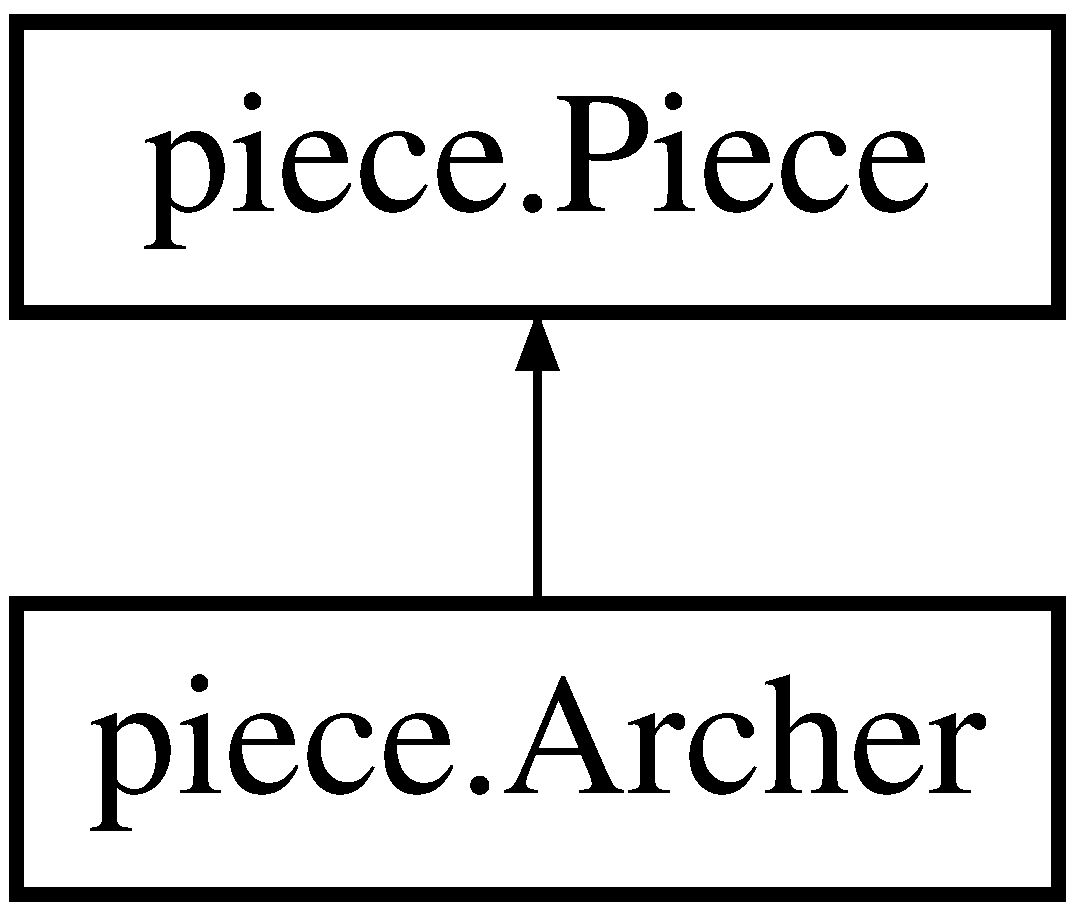
\includegraphics[height=2.000000cm]{classpiece_1_1_archer}
\end{center}
\end{figure}
\subsection*{Public Member Functions}
\begin{DoxyCompactItemize}
\item 
\hyperlink{classpiece_1_1_archer_a0a99d10d9c827a180e8743ec10489344}{Archer} (\hyperlink{classchessboard_1_1_chess_board}{Chess\+Board} board, \hyperlink{enumchessboard_1_1_player}{Player} player)
\item 
void \hyperlink{classpiece_1_1_archer_ae536059b2403dfe1ca315b8166d90c45}{add\+To\+Coord\+If\+There\+Is\+Enemy} (Array\+List$<$ \hyperlink{classpiece_1_1_coordinate}{Coordinate} $>$ coords, int x, int y)
\item 
Array\+List$<$ \hyperlink{classpiece_1_1_coordinate}{Coordinate} $>$ \hyperlink{classpiece_1_1_archer_afaddadc53c41508da32f6c14e5e57317}{get\+Possible\+Move\+Coordinate} ()
\end{DoxyCompactItemize}
\subsection*{Additional Inherited Members}


\subsection{Detailed Description}
Created by wangyiyi on 2/18/15. 

\subsection{Constructor \& Destructor Documentation}
\hypertarget{classpiece_1_1_archer_a0a99d10d9c827a180e8743ec10489344}{}\index{piece\+::\+Archer@{piece\+::\+Archer}!Archer@{Archer}}
\index{Archer@{Archer}!piece\+::\+Archer@{piece\+::\+Archer}}
\subsubsection[{Archer}]{\setlength{\rightskip}{0pt plus 5cm}piece.\+Archer.\+Archer (
\begin{DoxyParamCaption}
\item[{{\bf Chess\+Board}}]{board, }
\item[{{\bf Player}}]{player}
\end{DoxyParamCaption}
)\hspace{0.3cm}{\ttfamily [inline]}}\label{classpiece_1_1_archer_a0a99d10d9c827a180e8743ec10489344}
Constructor\+: initialize an Archor Object 
\begin{DoxyParams}{Parameters}
{\em board} & the board we are currently using \\
\hline
{\em player} & the player holds this piece \\
\hline
\end{DoxyParams}


\subsection{Member Function Documentation}
\hypertarget{classpiece_1_1_archer_ae536059b2403dfe1ca315b8166d90c45}{}\index{piece\+::\+Archer@{piece\+::\+Archer}!add\+To\+Coord\+If\+There\+Is\+Enemy@{add\+To\+Coord\+If\+There\+Is\+Enemy}}
\index{add\+To\+Coord\+If\+There\+Is\+Enemy@{add\+To\+Coord\+If\+There\+Is\+Enemy}!piece\+::\+Archer@{piece\+::\+Archer}}
\subsubsection[{add\+To\+Coord\+If\+There\+Is\+Enemy}]{\setlength{\rightskip}{0pt plus 5cm}void piece.\+Archer.\+add\+To\+Coord\+If\+There\+Is\+Enemy (
\begin{DoxyParamCaption}
\item[{Array\+List$<$ {\bf Coordinate} $>$}]{coords, }
\item[{int}]{x, }
\item[{int}]{y}
\end{DoxyParamCaption}
)\hspace{0.3cm}{\ttfamily [inline]}}\label{classpiece_1_1_archer_ae536059b2403dfe1ca315b8166d90c45}
add (x, y) to coords if there is enemy 
\begin{DoxyParams}{Parameters}
{\em x} & the x coordinate \\
\hline
{\em y} & the y coordinate \\
\hline
\end{DoxyParams}
\hypertarget{classpiece_1_1_archer_afaddadc53c41508da32f6c14e5e57317}{}\index{piece\+::\+Archer@{piece\+::\+Archer}!get\+Possible\+Move\+Coordinate@{get\+Possible\+Move\+Coordinate}}
\index{get\+Possible\+Move\+Coordinate@{get\+Possible\+Move\+Coordinate}!piece\+::\+Archer@{piece\+::\+Archer}}
\subsubsection[{get\+Possible\+Move\+Coordinate}]{\setlength{\rightskip}{0pt plus 5cm}Array\+List$<${\bf Coordinate}$>$ piece.\+Archer.\+get\+Possible\+Move\+Coordinate (
\begin{DoxyParamCaption}
{}
\end{DoxyParamCaption}
)\hspace{0.3cm}{\ttfamily [inline]}}\label{classpiece_1_1_archer_afaddadc53c41508da32f6c14e5e57317}
Attack and Move coordinate\+: \begin{DoxyVerb}    # # #                #: is enemy
  #   @   #              @: is possible move area
  # @ P @ #              P: archer
  #   @   #
    # # #
\end{DoxyVerb}


\begin{DoxyReturn}{Returns}
Array\+List$<$\+Coordinate$>$ Object that contains all possible move coordinates. 
\end{DoxyReturn}


The documentation for this class was generated from the following file\+:\begin{DoxyCompactItemize}
\item 
src/piece/Archer.\+java\end{DoxyCompactItemize}

\hypertarget{classunit__test_1_1_archer_test}{}\section{unit\+\_\+test.\+Archer\+Test Class Reference}
\label{classunit__test_1_1_archer_test}\index{unit\+\_\+test.\+Archer\+Test@{unit\+\_\+test.\+Archer\+Test}}
Inheritance diagram for unit\+\_\+test.\+Archer\+Test\+:\begin{figure}[H]
\begin{center}
\leavevmode
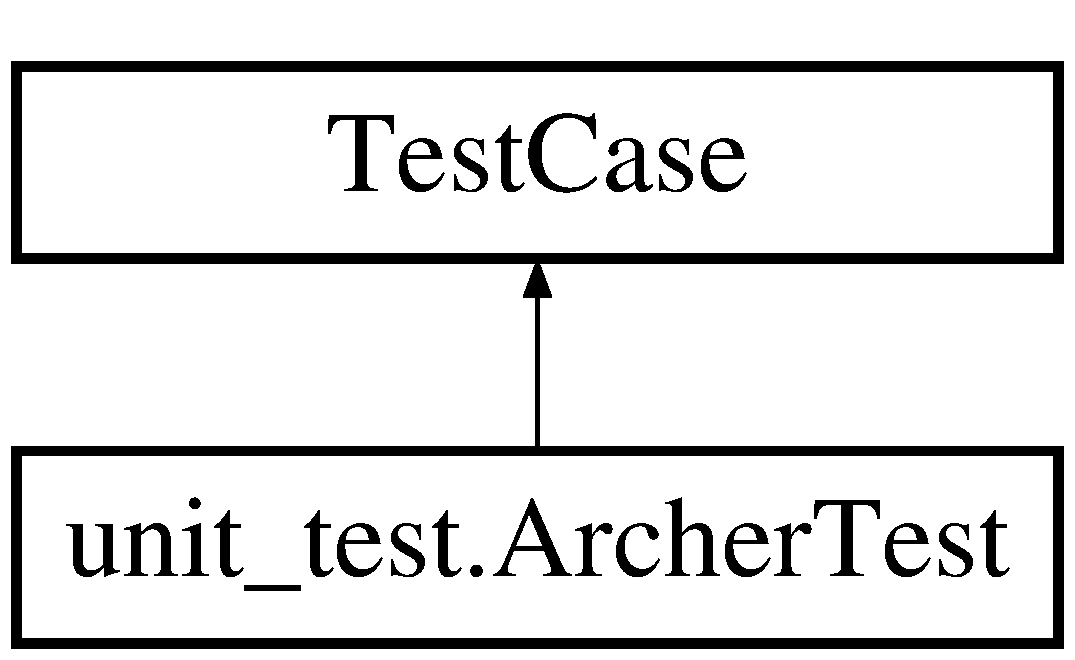
\includegraphics[height=2.000000cm]{classunit__test_1_1_archer_test}
\end{center}
\end{figure}
\subsection*{Public Member Functions}
\begin{DoxyCompactItemize}
\item 
void \hyperlink{classunit__test_1_1_archer_test_a473613443a8cedacab12c380fc5fb21b}{test\+Get\+Possible\+Move\+Coordinate} ()  throws Exception 
\end{DoxyCompactItemize}


\subsection{Member Function Documentation}
\hypertarget{classunit__test_1_1_archer_test_a473613443a8cedacab12c380fc5fb21b}{}\index{unit\+\_\+test\+::\+Archer\+Test@{unit\+\_\+test\+::\+Archer\+Test}!test\+Get\+Possible\+Move\+Coordinate@{test\+Get\+Possible\+Move\+Coordinate}}
\index{test\+Get\+Possible\+Move\+Coordinate@{test\+Get\+Possible\+Move\+Coordinate}!unit\+\_\+test\+::\+Archer\+Test@{unit\+\_\+test\+::\+Archer\+Test}}
\subsubsection[{test\+Get\+Possible\+Move\+Coordinate}]{\setlength{\rightskip}{0pt plus 5cm}void unit\+\_\+test.\+Archer\+Test.\+test\+Get\+Possible\+Move\+Coordinate (
\begin{DoxyParamCaption}
{}
\end{DoxyParamCaption}
) throws Exception\hspace{0.3cm}{\ttfamily [inline]}}\label{classunit__test_1_1_archer_test_a473613443a8cedacab12c380fc5fb21b}
test valid possible moves 

The documentation for this class was generated from the following file\+:\begin{DoxyCompactItemize}
\item 
unit\+\_\+test/Archer\+Test.\+java\end{DoxyCompactItemize}

\hypertarget{classpiece_1_1_bishop}{}\section{piece.\+Bishop Class Reference}
\label{classpiece_1_1_bishop}\index{piece.\+Bishop@{piece.\+Bishop}}
Inheritance diagram for piece.\+Bishop\+:\begin{figure}[H]
\begin{center}
\leavevmode
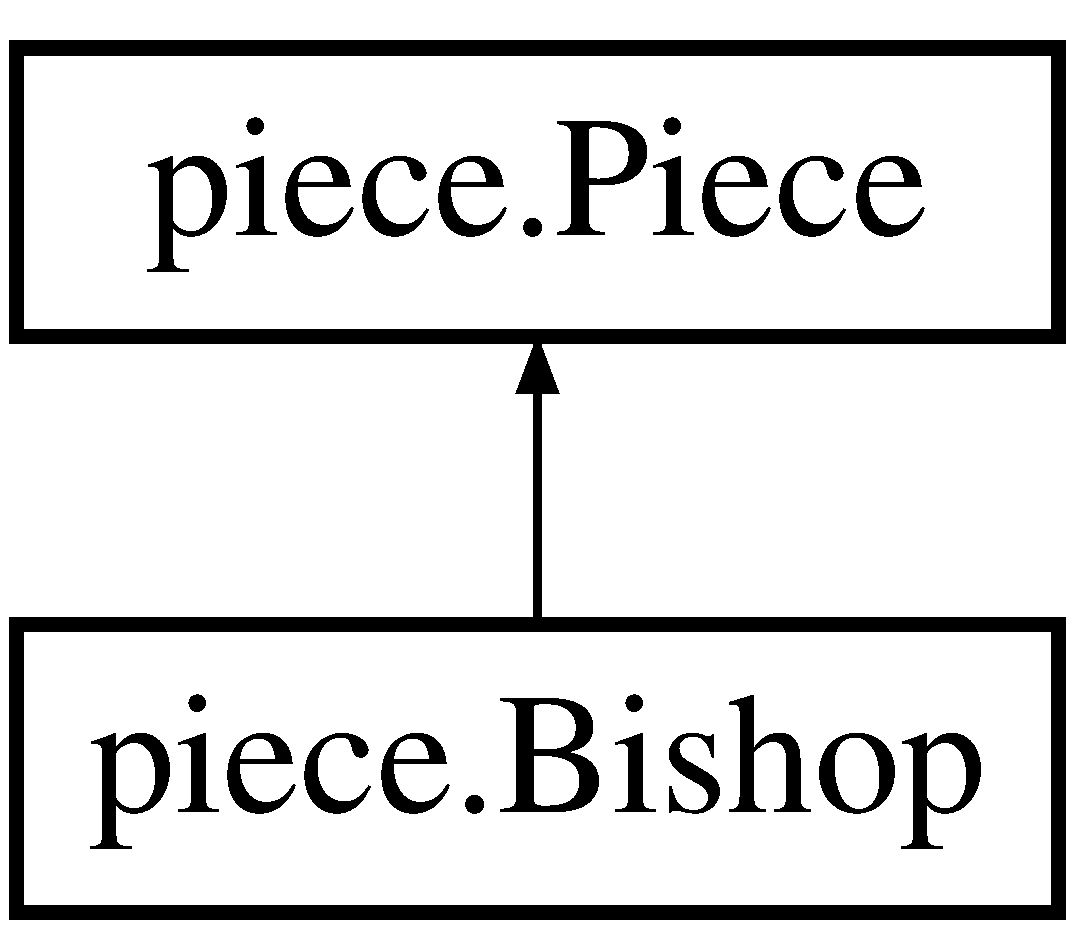
\includegraphics[height=2.000000cm]{classpiece_1_1_bishop}
\end{center}
\end{figure}
\subsection*{Public Member Functions}
\begin{DoxyCompactItemize}
\item 
\hyperlink{classpiece_1_1_bishop_ac48ed9faad6e77272086e3d6bce54244}{Bishop} (\hyperlink{classchess_1_1_chess_board}{Chess\+Board} board, \hyperlink{enumchess_1_1_player}{Player} player)
\item 
Array\+List$<$ \hyperlink{classpiece_1_1_coordinate}{Coordinate} $>$ \hyperlink{classpiece_1_1_bishop_aee0c8f13e3014881bb397a48bfce4ccf}{get\+Possible\+Move\+Coordinate} ()
\end{DoxyCompactItemize}
\subsection*{Additional Inherited Members}


\subsection{Detailed Description}
Created by wangyiyi on 2/12/15. 

\subsection{Constructor \& Destructor Documentation}
\hypertarget{classpiece_1_1_bishop_ac48ed9faad6e77272086e3d6bce54244}{}\index{piece\+::\+Bishop@{piece\+::\+Bishop}!Bishop@{Bishop}}
\index{Bishop@{Bishop}!piece\+::\+Bishop@{piece\+::\+Bishop}}
\subsubsection[{Bishop}]{\setlength{\rightskip}{0pt plus 5cm}piece.\+Bishop.\+Bishop (
\begin{DoxyParamCaption}
\item[{{\bf Chess\+Board}}]{board, }
\item[{{\bf Player}}]{player}
\end{DoxyParamCaption}
)\hspace{0.3cm}{\ttfamily [inline]}}\label{classpiece_1_1_bishop_ac48ed9faad6e77272086e3d6bce54244}
Constructor\+: initialize a \hyperlink{classpiece_1_1_bishop}{Bishop} Object 
\begin{DoxyParams}{Parameters}
{\em board} & \\
\hline
{\em player} & \\
\hline
\end{DoxyParams}


\subsection{Member Function Documentation}
\hypertarget{classpiece_1_1_bishop_aee0c8f13e3014881bb397a48bfce4ccf}{}\index{piece\+::\+Bishop@{piece\+::\+Bishop}!get\+Possible\+Move\+Coordinate@{get\+Possible\+Move\+Coordinate}}
\index{get\+Possible\+Move\+Coordinate@{get\+Possible\+Move\+Coordinate}!piece\+::\+Bishop@{piece\+::\+Bishop}}
\subsubsection[{get\+Possible\+Move\+Coordinate}]{\setlength{\rightskip}{0pt plus 5cm}Array\+List$<${\bf Coordinate}$>$ piece.\+Bishop.\+get\+Possible\+Move\+Coordinate (
\begin{DoxyParamCaption}
{}
\end{DoxyParamCaption}
)\hspace{0.3cm}{\ttfamily [inline]}}\label{classpiece_1_1_bishop_aee0c8f13e3014881bb397a48bfce4ccf}
Get all possible move coordinates for this bishop piece at current coordinate @ @ @ @ P\+: this piece @ @ @\+: Possible coordinates to move @ @ @ @ P @ @ @ @ @ @ @ @

\begin{DoxyReturn}{Returns}
Array\+List$<$\+Coordinate$>$ Object 
\end{DoxyReturn}


The documentation for this class was generated from the following file\+:\begin{DoxyCompactItemize}
\item 
piece/Bishop.\+java\end{DoxyCompactItemize}

\hypertarget{classunit__test_1_1_bishop_test}{}\section{unit\+\_\+test.\+Bishop\+Test Class Reference}
\label{classunit__test_1_1_bishop_test}\index{unit\+\_\+test.\+Bishop\+Test@{unit\+\_\+test.\+Bishop\+Test}}
\subsection*{Public Member Functions}
\begin{DoxyCompactItemize}
\item 
void \hyperlink{classunit__test_1_1_bishop_test_a2864b3553e1f235dcd095d9f02ff6978}{test\+Get\+Possible\+Move\+Coordinate} ()  throws Exception 
\end{DoxyCompactItemize}


\subsection{Member Function Documentation}
\hypertarget{classunit__test_1_1_bishop_test_a2864b3553e1f235dcd095d9f02ff6978}{}\index{unit\+\_\+test\+::\+Bishop\+Test@{unit\+\_\+test\+::\+Bishop\+Test}!test\+Get\+Possible\+Move\+Coordinate@{test\+Get\+Possible\+Move\+Coordinate}}
\index{test\+Get\+Possible\+Move\+Coordinate@{test\+Get\+Possible\+Move\+Coordinate}!unit\+\_\+test\+::\+Bishop\+Test@{unit\+\_\+test\+::\+Bishop\+Test}}
\subsubsection[{test\+Get\+Possible\+Move\+Coordinate}]{\setlength{\rightskip}{0pt plus 5cm}void unit\+\_\+test.\+Bishop\+Test.\+test\+Get\+Possible\+Move\+Coordinate (
\begin{DoxyParamCaption}
{}
\end{DoxyParamCaption}
) throws Exception\hspace{0.3cm}{\ttfamily [inline]}}\label{classunit__test_1_1_bishop_test_a2864b3553e1f235dcd095d9f02ff6978}
test valid possible moves 

The documentation for this class was generated from the following file\+:\begin{DoxyCompactItemize}
\item 
src/unit\+\_\+test/Bishop\+Test.\+java\end{DoxyCompactItemize}

\hypertarget{classchessboard_1_1_chess_board}{}\section{chessboard.\+Chess\+Board Class Reference}
\label{classchessboard_1_1_chess_board}\index{chessboard.\+Chess\+Board@{chessboard.\+Chess\+Board}}
\subsection*{Public Member Functions}
\begin{DoxyCompactItemize}
\item 
\hyperlink{classchessboard_1_1_chess_board_a38aa6904871b6262948c855ade0eca00}{Chess\+Board} (int width, int height)
\item 
void \hyperlink{classchessboard_1_1_chess_board_a15c0c36e6095d524ac240559bcba55e0}{add\+Piece\+To\+List} (\hyperlink{classpiece_1_1_piece}{Piece} p)
\item 
Array\+List$<$ \hyperlink{classpiece_1_1_piece}{Piece} $>$ \hyperlink{classchessboard_1_1_chess_board_acc14cc7fad0cda996d1490fedb0188c5}{get\+White\+\_\+pieces} ()
\item 
Array\+List$<$ \hyperlink{classpiece_1_1_piece}{Piece} $>$ \hyperlink{classchessboard_1_1_chess_board_a8dc0208b60329e17af4e8f55200cfb50}{get\+Black\+\_\+pieces} ()
\item 
\hyperlink{classpiece_1_1_piece}{Piece} \hyperlink{classchessboard_1_1_chess_board_a4ef0d142d0b958c54b9ba5eadeffea87}{get\+King1} ()
\item 
void \hyperlink{classchessboard_1_1_chess_board_a22934b1f0864cca03bbbe47fbc788a60}{set\+King1} (\hyperlink{classpiece_1_1_piece}{Piece} p)
\item 
\hyperlink{classpiece_1_1_piece}{Piece} \hyperlink{classchessboard_1_1_chess_board_a23cacc50525158666322a65b4bf6bbcb}{get\+King2} ()
\item 
void \hyperlink{classchessboard_1_1_chess_board_a720f9ecb8d6aeb8795597b75ba19ac4b}{set\+King2} (\hyperlink{classpiece_1_1_piece}{Piece} p)
\item 
\hyperlink{classpiece_1_1_piece}{Piece} \hyperlink{classchessboard_1_1_chess_board_a468f723b34b4985741131377c093411a}{get\+Piece\+At\+Coordinate} (int x, int y)
\item 
void \hyperlink{classchessboard_1_1_chess_board_a6784a7de408948edcd83d0bccc5a5642}{set\+Piece\+At\+Coordinate} (\hyperlink{classpiece_1_1_piece}{Piece} p, int x, int y)
\item 
int \hyperlink{classchessboard_1_1_chess_board_a8dfab964b5ad169064a62363bc7d0b04}{get\+Width} ()
\item 
int \hyperlink{classchessboard_1_1_chess_board_a2357c65378bac8ae24846f4d122bd3eb}{get\+Height} ()
\item 
void \hyperlink{classchessboard_1_1_chess_board_a657610e54b48f68c96c52af0170e0d82}{remove\+Piece} (\hyperlink{classpiece_1_1_piece}{Piece} p)
\item 
void \hyperlink{classchessboard_1_1_chess_board_a7f80c079e2bbd4e538ceb3b3ad0be81f}{set\+Turns} (int turns)
\item 
void \hyperlink{classchessboard_1_1_chess_board_a25e5bfbfe9f7bb1ccecd2e6b6b7c535d}{increment\+Turns} ()
\item 
int \hyperlink{classchessboard_1_1_chess_board_a535dad0864d10c1a2f11bcb1cec2e1ec}{get\+Turns} ()
\item 
\hyperlink{enumchessboard_1_1_player}{Player} \hyperlink{classchessboard_1_1_chess_board_a9eaa26069854d00d362071ed7dfe6ff1}{get\+Player\+For\+This\+Turn} ()
\item 
boolean \hyperlink{classchessboard_1_1_chess_board_add7b556d1e52a4ec70c2dc9154c587a2}{player\+Cannot\+Move} (\hyperlink{enumchessboard_1_1_player}{Player} player)
\item 
boolean \hyperlink{classchessboard_1_1_chess_board_a54ce6f2b74db08e4ed2e11982ca396c7}{is\+Stalemate} (\hyperlink{enumchessboard_1_1_player}{Player} player)
\item 
void \hyperlink{classchessboard_1_1_chess_board_a7f81546419328da5580d87e24bfed804}{generate\+Standard\+Board} ()
\item 
void \hyperlink{classchessboard_1_1_chess_board_a70b0f46299f574a5ef465105fefcfb08}{generate\+Fantasy\+Board} ()
\end{DoxyCompactItemize}
\subsection*{Protected Attributes}
\begin{DoxyCompactItemize}
\item 
\hypertarget{classchessboard_1_1_chess_board_a550e6dddb19052e0b3759a2f6ced4f62}{}int {\bfseries width}\label{classchessboard_1_1_chess_board_a550e6dddb19052e0b3759a2f6ced4f62}

\item 
\hypertarget{classchessboard_1_1_chess_board_ad67be26cc8ba04f4deffe3ca7e8c2313}{}int {\bfseries height}\label{classchessboard_1_1_chess_board_ad67be26cc8ba04f4deffe3ca7e8c2313}

\item 
\hypertarget{classchessboard_1_1_chess_board_a30976a4382c751ed5f6dea0c4bab2df3}{}\hyperlink{classpiece_1_1_piece}{Piece} {\bfseries king1}\label{classchessboard_1_1_chess_board_a30976a4382c751ed5f6dea0c4bab2df3}

\item 
\hypertarget{classchessboard_1_1_chess_board_a05f244efe3c9816d81886fecb0de109a}{}\hyperlink{classpiece_1_1_piece}{Piece} {\bfseries king2}\label{classchessboard_1_1_chess_board_a05f244efe3c9816d81886fecb0de109a}

\item 
\hypertarget{classchessboard_1_1_chess_board_a2c230cbaa43e859ce5c455d71f2ca1a9}{}int {\bfseries turns}\label{classchessboard_1_1_chess_board_a2c230cbaa43e859ce5c455d71f2ca1a9}

\end{DoxyCompactItemize}


\subsection{Detailed Description}
Created by wangyiyi on 2/12/15. This is the chessboard class(\+Model) 

\subsection{Constructor \& Destructor Documentation}
\hypertarget{classchessboard_1_1_chess_board_a38aa6904871b6262948c855ade0eca00}{}\index{chessboard\+::\+Chess\+Board@{chessboard\+::\+Chess\+Board}!Chess\+Board@{Chess\+Board}}
\index{Chess\+Board@{Chess\+Board}!chessboard\+::\+Chess\+Board@{chessboard\+::\+Chess\+Board}}
\subsubsection[{Chess\+Board}]{\setlength{\rightskip}{0pt plus 5cm}chessboard.\+Chess\+Board.\+Chess\+Board (
\begin{DoxyParamCaption}
\item[{int}]{width, }
\item[{int}]{height}
\end{DoxyParamCaption}
)\hspace{0.3cm}{\ttfamily [inline]}}\label{classchessboard_1_1_chess_board_a38aa6904871b6262948c855ade0eca00}
Construct chess board given width and height \begin{DoxyVerb} Coordinate system

 +
 |
 |
 |
 |
 (0, 0) -------->  +
\end{DoxyVerb}



\begin{DoxyParams}{Parameters}
{\em width} & set the width of chessboard \\
\hline
{\em height} & set the height of chessboard \\
\hline
\end{DoxyParams}


\subsection{Member Function Documentation}
\hypertarget{classchessboard_1_1_chess_board_a15c0c36e6095d524ac240559bcba55e0}{}\index{chessboard\+::\+Chess\+Board@{chessboard\+::\+Chess\+Board}!add\+Piece\+To\+List@{add\+Piece\+To\+List}}
\index{add\+Piece\+To\+List@{add\+Piece\+To\+List}!chessboard\+::\+Chess\+Board@{chessboard\+::\+Chess\+Board}}
\subsubsection[{add\+Piece\+To\+List}]{\setlength{\rightskip}{0pt plus 5cm}void chessboard.\+Chess\+Board.\+add\+Piece\+To\+List (
\begin{DoxyParamCaption}
\item[{{\bf Piece}}]{p}
\end{DoxyParamCaption}
)\hspace{0.3cm}{\ttfamily [inline]}}\label{classchessboard_1_1_chess_board_a15c0c36e6095d524ac240559bcba55e0}
add piece to white\+\_\+pieces or black\+\_\+pieces array list 
\begin{DoxyParams}{Parameters}
{\em p} & The piece we want to save. \\
\hline
\end{DoxyParams}
\hypertarget{classchessboard_1_1_chess_board_a70b0f46299f574a5ef465105fefcfb08}{}\index{chessboard\+::\+Chess\+Board@{chessboard\+::\+Chess\+Board}!generate\+Fantasy\+Board@{generate\+Fantasy\+Board}}
\index{generate\+Fantasy\+Board@{generate\+Fantasy\+Board}!chessboard\+::\+Chess\+Board@{chessboard\+::\+Chess\+Board}}
\subsubsection[{generate\+Fantasy\+Board}]{\setlength{\rightskip}{0pt plus 5cm}void chessboard.\+Chess\+Board.\+generate\+Fantasy\+Board (
\begin{DoxyParamCaption}
{}
\end{DoxyParamCaption}
)\hspace{0.3cm}{\ttfamily [inline]}}\label{classchessboard_1_1_chess_board_a70b0f46299f574a5ef465105fefcfb08}
Generate fantasy 8 x 8 chess board \hypertarget{classchessboard_1_1_chess_board_a7f81546419328da5580d87e24bfed804}{}\index{chessboard\+::\+Chess\+Board@{chessboard\+::\+Chess\+Board}!generate\+Standard\+Board@{generate\+Standard\+Board}}
\index{generate\+Standard\+Board@{generate\+Standard\+Board}!chessboard\+::\+Chess\+Board@{chessboard\+::\+Chess\+Board}}
\subsubsection[{generate\+Standard\+Board}]{\setlength{\rightskip}{0pt plus 5cm}void chessboard.\+Chess\+Board.\+generate\+Standard\+Board (
\begin{DoxyParamCaption}
{}
\end{DoxyParamCaption}
)\hspace{0.3cm}{\ttfamily [inline]}}\label{classchessboard_1_1_chess_board_a7f81546419328da5580d87e24bfed804}
Generate standard 8 x 8 chess board \hypertarget{classchessboard_1_1_chess_board_a8dc0208b60329e17af4e8f55200cfb50}{}\index{chessboard\+::\+Chess\+Board@{chessboard\+::\+Chess\+Board}!get\+Black\+\_\+pieces@{get\+Black\+\_\+pieces}}
\index{get\+Black\+\_\+pieces@{get\+Black\+\_\+pieces}!chessboard\+::\+Chess\+Board@{chessboard\+::\+Chess\+Board}}
\subsubsection[{get\+Black\+\_\+pieces}]{\setlength{\rightskip}{0pt plus 5cm}Array\+List$<${\bf Piece}$>$ chessboard.\+Chess\+Board.\+get\+Black\+\_\+pieces (
\begin{DoxyParamCaption}
{}
\end{DoxyParamCaption}
)\hspace{0.3cm}{\ttfamily [inline]}}\label{classchessboard_1_1_chess_board_a8dc0208b60329e17af4e8f55200cfb50}
Getter\+: return this.\+black\+\_\+pieces \begin{DoxyReturn}{Returns}
black\+\_\+piece array list that contains all black pieces 
\end{DoxyReturn}
\hypertarget{classchessboard_1_1_chess_board_a2357c65378bac8ae24846f4d122bd3eb}{}\index{chessboard\+::\+Chess\+Board@{chessboard\+::\+Chess\+Board}!get\+Height@{get\+Height}}
\index{get\+Height@{get\+Height}!chessboard\+::\+Chess\+Board@{chessboard\+::\+Chess\+Board}}
\subsubsection[{get\+Height}]{\setlength{\rightskip}{0pt plus 5cm}int chessboard.\+Chess\+Board.\+get\+Height (
\begin{DoxyParamCaption}
{}
\end{DoxyParamCaption}
)\hspace{0.3cm}{\ttfamily [inline]}}\label{classchessboard_1_1_chess_board_a2357c65378bac8ae24846f4d122bd3eb}
Getter\+: get the height of chessboard \begin{DoxyReturn}{Returns}
the height of chessboard 
\end{DoxyReturn}
\hypertarget{classchessboard_1_1_chess_board_a4ef0d142d0b958c54b9ba5eadeffea87}{}\index{chessboard\+::\+Chess\+Board@{chessboard\+::\+Chess\+Board}!get\+King1@{get\+King1}}
\index{get\+King1@{get\+King1}!chessboard\+::\+Chess\+Board@{chessboard\+::\+Chess\+Board}}
\subsubsection[{get\+King1}]{\setlength{\rightskip}{0pt plus 5cm}{\bf Piece} chessboard.\+Chess\+Board.\+get\+King1 (
\begin{DoxyParamCaption}
{}
\end{DoxyParamCaption}
)\hspace{0.3cm}{\ttfamily [inline]}}\label{classchessboard_1_1_chess_board_a4ef0d142d0b958c54b9ba5eadeffea87}
Getter\+: get king1 from W\+H\+I\+T\+E player \begin{DoxyReturn}{Returns}
king piece from W\+H\+I\+T\+E player 
\end{DoxyReturn}
\hypertarget{classchessboard_1_1_chess_board_a23cacc50525158666322a65b4bf6bbcb}{}\index{chessboard\+::\+Chess\+Board@{chessboard\+::\+Chess\+Board}!get\+King2@{get\+King2}}
\index{get\+King2@{get\+King2}!chessboard\+::\+Chess\+Board@{chessboard\+::\+Chess\+Board}}
\subsubsection[{get\+King2}]{\setlength{\rightskip}{0pt plus 5cm}{\bf Piece} chessboard.\+Chess\+Board.\+get\+King2 (
\begin{DoxyParamCaption}
{}
\end{DoxyParamCaption}
)\hspace{0.3cm}{\ttfamily [inline]}}\label{classchessboard_1_1_chess_board_a23cacc50525158666322a65b4bf6bbcb}
Getter\+: get king2 from B\+L\+A\+C\+K player \begin{DoxyReturn}{Returns}
king piece from B\+L\+A\+C\+K player 
\end{DoxyReturn}
\hypertarget{classchessboard_1_1_chess_board_a468f723b34b4985741131377c093411a}{}\index{chessboard\+::\+Chess\+Board@{chessboard\+::\+Chess\+Board}!get\+Piece\+At\+Coordinate@{get\+Piece\+At\+Coordinate}}
\index{get\+Piece\+At\+Coordinate@{get\+Piece\+At\+Coordinate}!chessboard\+::\+Chess\+Board@{chessboard\+::\+Chess\+Board}}
\subsubsection[{get\+Piece\+At\+Coordinate}]{\setlength{\rightskip}{0pt plus 5cm}{\bf Piece} chessboard.\+Chess\+Board.\+get\+Piece\+At\+Coordinate (
\begin{DoxyParamCaption}
\item[{int}]{x, }
\item[{int}]{y}
\end{DoxyParamCaption}
)\hspace{0.3cm}{\ttfamily [inline]}}\label{classchessboard_1_1_chess_board_a468f723b34b4985741131377c093411a}
Return the piece at given coordinate if there is no piece at that coordinate, or that coordinate is invalid, return null 
\begin{DoxyParams}{Parameters}
{\em x} & the x coordinate \\
\hline
{\em y} & the y coordinate \\
\hline
\end{DoxyParams}
\begin{DoxyReturn}{Returns}
the piece at that (x, y) coordinate. If coordinate not valid, return null. 
\end{DoxyReturn}
\hypertarget{classchessboard_1_1_chess_board_a9eaa26069854d00d362071ed7dfe6ff1}{}\index{chessboard\+::\+Chess\+Board@{chessboard\+::\+Chess\+Board}!get\+Player\+For\+This\+Turn@{get\+Player\+For\+This\+Turn}}
\index{get\+Player\+For\+This\+Turn@{get\+Player\+For\+This\+Turn}!chessboard\+::\+Chess\+Board@{chessboard\+::\+Chess\+Board}}
\subsubsection[{get\+Player\+For\+This\+Turn}]{\setlength{\rightskip}{0pt plus 5cm}{\bf Player} chessboard.\+Chess\+Board.\+get\+Player\+For\+This\+Turn (
\begin{DoxyParamCaption}
{}
\end{DoxyParamCaption}
)\hspace{0.3cm}{\ttfamily [inline]}}\label{classchessboard_1_1_chess_board_a9eaa26069854d00d362071ed7dfe6ff1}
Get the player for this turn \begin{DoxyReturn}{Returns}
the player for this turn 
\end{DoxyReturn}
\hypertarget{classchessboard_1_1_chess_board_a535dad0864d10c1a2f11bcb1cec2e1ec}{}\index{chessboard\+::\+Chess\+Board@{chessboard\+::\+Chess\+Board}!get\+Turns@{get\+Turns}}
\index{get\+Turns@{get\+Turns}!chessboard\+::\+Chess\+Board@{chessboard\+::\+Chess\+Board}}
\subsubsection[{get\+Turns}]{\setlength{\rightskip}{0pt plus 5cm}int chessboard.\+Chess\+Board.\+get\+Turns (
\begin{DoxyParamCaption}
{}
\end{DoxyParamCaption}
)\hspace{0.3cm}{\ttfamily [inline]}}\label{classchessboard_1_1_chess_board_a535dad0864d10c1a2f11bcb1cec2e1ec}
Getter\+: get turns \begin{DoxyReturn}{Returns}
turns of the game 
\end{DoxyReturn}
\hypertarget{classchessboard_1_1_chess_board_acc14cc7fad0cda996d1490fedb0188c5}{}\index{chessboard\+::\+Chess\+Board@{chessboard\+::\+Chess\+Board}!get\+White\+\_\+pieces@{get\+White\+\_\+pieces}}
\index{get\+White\+\_\+pieces@{get\+White\+\_\+pieces}!chessboard\+::\+Chess\+Board@{chessboard\+::\+Chess\+Board}}
\subsubsection[{get\+White\+\_\+pieces}]{\setlength{\rightskip}{0pt plus 5cm}Array\+List$<${\bf Piece}$>$ chessboard.\+Chess\+Board.\+get\+White\+\_\+pieces (
\begin{DoxyParamCaption}
{}
\end{DoxyParamCaption}
)\hspace{0.3cm}{\ttfamily [inline]}}\label{classchessboard_1_1_chess_board_acc14cc7fad0cda996d1490fedb0188c5}
Getter\+: return this.\+white\+\_\+pieces \begin{DoxyReturn}{Returns}
white\+\_\+piece array list that contains all white pieces 
\end{DoxyReturn}
\hypertarget{classchessboard_1_1_chess_board_a8dfab964b5ad169064a62363bc7d0b04}{}\index{chessboard\+::\+Chess\+Board@{chessboard\+::\+Chess\+Board}!get\+Width@{get\+Width}}
\index{get\+Width@{get\+Width}!chessboard\+::\+Chess\+Board@{chessboard\+::\+Chess\+Board}}
\subsubsection[{get\+Width}]{\setlength{\rightskip}{0pt plus 5cm}int chessboard.\+Chess\+Board.\+get\+Width (
\begin{DoxyParamCaption}
{}
\end{DoxyParamCaption}
)\hspace{0.3cm}{\ttfamily [inline]}}\label{classchessboard_1_1_chess_board_a8dfab964b5ad169064a62363bc7d0b04}
Getter\+: get the width of chessboard \begin{DoxyReturn}{Returns}
the width of chessboard 
\end{DoxyReturn}
\hypertarget{classchessboard_1_1_chess_board_a25e5bfbfe9f7bb1ccecd2e6b6b7c535d}{}\index{chessboard\+::\+Chess\+Board@{chessboard\+::\+Chess\+Board}!increment\+Turns@{increment\+Turns}}
\index{increment\+Turns@{increment\+Turns}!chessboard\+::\+Chess\+Board@{chessboard\+::\+Chess\+Board}}
\subsubsection[{increment\+Turns}]{\setlength{\rightskip}{0pt plus 5cm}void chessboard.\+Chess\+Board.\+increment\+Turns (
\begin{DoxyParamCaption}
{}
\end{DoxyParamCaption}
)\hspace{0.3cm}{\ttfamily [inline]}}\label{classchessboard_1_1_chess_board_a25e5bfbfe9f7bb1ccecd2e6b6b7c535d}
Increment turns by 1 \hypertarget{classchessboard_1_1_chess_board_a54ce6f2b74db08e4ed2e11982ca396c7}{}\index{chessboard\+::\+Chess\+Board@{chessboard\+::\+Chess\+Board}!is\+Stalemate@{is\+Stalemate}}
\index{is\+Stalemate@{is\+Stalemate}!chessboard\+::\+Chess\+Board@{chessboard\+::\+Chess\+Board}}
\subsubsection[{is\+Stalemate}]{\setlength{\rightskip}{0pt plus 5cm}boolean chessboard.\+Chess\+Board.\+is\+Stalemate (
\begin{DoxyParamCaption}
\item[{{\bf Player}}]{player}
\end{DoxyParamCaption}
)\hspace{0.3cm}{\ttfamily [inline]}}\label{classchessboard_1_1_chess_board_a54ce6f2b74db08e4ed2e11982ca396c7}
Check whether player\textquotesingle{}s king is in stalemate.

when not checked, check whether is there any legal move.

if there is no legal move, return true; otherwise return false. 
\begin{DoxyParams}{Parameters}
{\em player} & \\
\hline
\end{DoxyParams}
\begin{DoxyReturn}{Returns}
true if there is stalemate; otherwise return false. 
\end{DoxyReturn}
\hypertarget{classchessboard_1_1_chess_board_add7b556d1e52a4ec70c2dc9154c587a2}{}\index{chessboard\+::\+Chess\+Board@{chessboard\+::\+Chess\+Board}!player\+Cannot\+Move@{player\+Cannot\+Move}}
\index{player\+Cannot\+Move@{player\+Cannot\+Move}!chessboard\+::\+Chess\+Board@{chessboard\+::\+Chess\+Board}}
\subsubsection[{player\+Cannot\+Move}]{\setlength{\rightskip}{0pt plus 5cm}boolean chessboard.\+Chess\+Board.\+player\+Cannot\+Move (
\begin{DoxyParamCaption}
\item[{{\bf Player}}]{player}
\end{DoxyParamCaption}
)\hspace{0.3cm}{\ttfamily [inline]}}\label{classchessboard_1_1_chess_board_add7b556d1e52a4ec70c2dc9154c587a2}
Check whether player can move a piece

If a player can not move any piece, then return true


\begin{DoxyParams}{Parameters}
{\em player} & check whether player can move a piece or not. \\
\hline
\end{DoxyParams}
\begin{DoxyReturn}{Returns}
return true if player cannot move any piece; otherwise return false 
\end{DoxyReturn}
\hypertarget{classchessboard_1_1_chess_board_a657610e54b48f68c96c52af0170e0d82}{}\index{chessboard\+::\+Chess\+Board@{chessboard\+::\+Chess\+Board}!remove\+Piece@{remove\+Piece}}
\index{remove\+Piece@{remove\+Piece}!chessboard\+::\+Chess\+Board@{chessboard\+::\+Chess\+Board}}
\subsubsection[{remove\+Piece}]{\setlength{\rightskip}{0pt plus 5cm}void chessboard.\+Chess\+Board.\+remove\+Piece (
\begin{DoxyParamCaption}
\item[{{\bf Piece}}]{p}
\end{DoxyParamCaption}
)\hspace{0.3cm}{\ttfamily [inline]}}\label{classchessboard_1_1_chess_board_a657610e54b48f68c96c52af0170e0d82}
Remove a piece from the chessboard 
\begin{DoxyParams}{Parameters}
{\em p} & the piece we want to remove from chessboard \\
\hline
\end{DoxyParams}
\hypertarget{classchessboard_1_1_chess_board_a22934b1f0864cca03bbbe47fbc788a60}{}\index{chessboard\+::\+Chess\+Board@{chessboard\+::\+Chess\+Board}!set\+King1@{set\+King1}}
\index{set\+King1@{set\+King1}!chessboard\+::\+Chess\+Board@{chessboard\+::\+Chess\+Board}}
\subsubsection[{set\+King1}]{\setlength{\rightskip}{0pt plus 5cm}void chessboard.\+Chess\+Board.\+set\+King1 (
\begin{DoxyParamCaption}
\item[{{\bf Piece}}]{p}
\end{DoxyParamCaption}
)\hspace{0.3cm}{\ttfamily [inline]}}\label{classchessboard_1_1_chess_board_a22934b1f0864cca03bbbe47fbc788a60}
Setter\+: set king1 
\begin{DoxyParams}{Parameters}
{\em p} & \\
\hline
\end{DoxyParams}
\hypertarget{classchessboard_1_1_chess_board_a720f9ecb8d6aeb8795597b75ba19ac4b}{}\index{chessboard\+::\+Chess\+Board@{chessboard\+::\+Chess\+Board}!set\+King2@{set\+King2}}
\index{set\+King2@{set\+King2}!chessboard\+::\+Chess\+Board@{chessboard\+::\+Chess\+Board}}
\subsubsection[{set\+King2}]{\setlength{\rightskip}{0pt plus 5cm}void chessboard.\+Chess\+Board.\+set\+King2 (
\begin{DoxyParamCaption}
\item[{{\bf Piece}}]{p}
\end{DoxyParamCaption}
)\hspace{0.3cm}{\ttfamily [inline]}}\label{classchessboard_1_1_chess_board_a720f9ecb8d6aeb8795597b75ba19ac4b}
Setter\+: set king2 
\begin{DoxyParams}{Parameters}
{\em p} & \\
\hline
\end{DoxyParams}
\hypertarget{classchessboard_1_1_chess_board_a6784a7de408948edcd83d0bccc5a5642}{}\index{chessboard\+::\+Chess\+Board@{chessboard\+::\+Chess\+Board}!set\+Piece\+At\+Coordinate@{set\+Piece\+At\+Coordinate}}
\index{set\+Piece\+At\+Coordinate@{set\+Piece\+At\+Coordinate}!chessboard\+::\+Chess\+Board@{chessboard\+::\+Chess\+Board}}
\subsubsection[{set\+Piece\+At\+Coordinate}]{\setlength{\rightskip}{0pt plus 5cm}void chessboard.\+Chess\+Board.\+set\+Piece\+At\+Coordinate (
\begin{DoxyParamCaption}
\item[{{\bf Piece}}]{p, }
\item[{int}]{x, }
\item[{int}]{y}
\end{DoxyParamCaption}
)\hspace{0.3cm}{\ttfamily [inline]}}\label{classchessboard_1_1_chess_board_a6784a7de408948edcd83d0bccc5a5642}
Store the piece at (x, y) coordinate 
\begin{DoxyParams}{Parameters}
{\em p} & the piece we want to set \\
\hline
{\em x} & the x coordinate \\
\hline
{\em y} & the y coordinate \\
\hline
\end{DoxyParams}
\hypertarget{classchessboard_1_1_chess_board_a7f80c079e2bbd4e538ceb3b3ad0be81f}{}\index{chessboard\+::\+Chess\+Board@{chessboard\+::\+Chess\+Board}!set\+Turns@{set\+Turns}}
\index{set\+Turns@{set\+Turns}!chessboard\+::\+Chess\+Board@{chessboard\+::\+Chess\+Board}}
\subsubsection[{set\+Turns}]{\setlength{\rightskip}{0pt plus 5cm}void chessboard.\+Chess\+Board.\+set\+Turns (
\begin{DoxyParamCaption}
\item[{int}]{turns}
\end{DoxyParamCaption}
)\hspace{0.3cm}{\ttfamily [inline]}}\label{classchessboard_1_1_chess_board_a7f80c079e2bbd4e538ceb3b3ad0be81f}
Setter\+: set turns 
\begin{DoxyParams}{Parameters}
{\em turns} & \\
\hline
\end{DoxyParams}


The documentation for this class was generated from the following file\+:\begin{DoxyCompactItemize}
\item 
src/chessboard/Chess\+Board.\+java\end{DoxyCompactItemize}

\hypertarget{classchessboard_1_1_chessboard___log}{}\section{chessboard.\+Chessboard\+\_\+\+Log Class Reference}
\label{classchessboard_1_1_chessboard___log}\index{chessboard.\+Chessboard\+\_\+\+Log@{chessboard.\+Chessboard\+\_\+\+Log}}
\subsection*{Public Member Functions}
\begin{DoxyCompactItemize}
\item 
\hyperlink{classchessboard_1_1_chessboard___log_a384258fcfa0ee1cdebc3aaeefbbb3b1e}{Chessboard\+\_\+\+Log} (\hyperlink{classchessboard_1_1_chess_board}{Chess\+Board} board)
\item 
\hyperlink{classchessboard_1_1_chess_board}{Chess\+Board} \hyperlink{classchessboard_1_1_chessboard___log_a3266897f1f2794261b6c34dc746913b9}{to\+Chessboard} ()
\item 
int \hyperlink{classchessboard_1_1_chessboard___log_a3969bceacf85592002a66eee9bc983c3}{get\+Turns} ()
\item 
int \hyperlink{classchessboard_1_1_chessboard___log_a8e81a3c0f7c83ea8c24c4266995923dc}{get\+Width} ()
\item 
int \hyperlink{classchessboard_1_1_chessboard___log_abb71e5ec723d33b2d5d4663af4f035b4}{get\+Height} ()
\item 
String \hyperlink{classchessboard_1_1_chessboard___log_a40c8d014f640fbb09da3c2ef4966c43c}{get\+Tile\+At\+Coordinate} (int x, int y)
\end{DoxyCompactItemize}
\subsection*{Protected Attributes}
\begin{DoxyCompactItemize}
\item 
\hypertarget{classchessboard_1_1_chessboard___log_a1307cb27af6ecddff06ebac5e29f30dc}{}int {\bfseries width}\label{classchessboard_1_1_chessboard___log_a1307cb27af6ecddff06ebac5e29f30dc}

\item 
\hypertarget{classchessboard_1_1_chessboard___log_adba869afdd69e27e54c22f4594435372}{}int {\bfseries height}\label{classchessboard_1_1_chessboard___log_adba869afdd69e27e54c22f4594435372}

\item 
\hypertarget{classchessboard_1_1_chessboard___log_a5c33c068bca1fe84b900c61a647b7cf7}{}String {\bfseries tiles} \mbox{[}$\,$\mbox{]}\mbox{[}$\,$\mbox{]}\label{classchessboard_1_1_chessboard___log_a5c33c068bca1fe84b900c61a647b7cf7}

\item 
\hypertarget{classchessboard_1_1_chessboard___log_a4ed9278cd6ff6478662abd0c2084401c}{}int {\bfseries turns}\label{classchessboard_1_1_chessboard___log_a4ed9278cd6ff6478662abd0c2084401c}

\end{DoxyCompactItemize}


\subsection{Detailed Description}
This class is used to save chessboard piece move history 

\subsection{Constructor \& Destructor Documentation}
\hypertarget{classchessboard_1_1_chessboard___log_a384258fcfa0ee1cdebc3aaeefbbb3b1e}{}\index{chessboard\+::\+Chessboard\+\_\+\+Log@{chessboard\+::\+Chessboard\+\_\+\+Log}!Chessboard\+\_\+\+Log@{Chessboard\+\_\+\+Log}}
\index{Chessboard\+\_\+\+Log@{Chessboard\+\_\+\+Log}!chessboard\+::\+Chessboard\+\_\+\+Log@{chessboard\+::\+Chessboard\+\_\+\+Log}}
\subsubsection[{Chessboard\+\_\+\+Log}]{\setlength{\rightskip}{0pt plus 5cm}chessboard.\+Chessboard\+\_\+\+Log.\+Chessboard\+\_\+\+Log (
\begin{DoxyParamCaption}
\item[{{\bf Chess\+Board}}]{board}
\end{DoxyParamCaption}
)\hspace{0.3cm}{\ttfamily [inline]}}\label{classchessboard_1_1_chessboard___log_a384258fcfa0ee1cdebc3aaeefbbb3b1e}
Generate chessboard log according to board 
\begin{DoxyParams}{Parameters}
{\em board} & \\
\hline
\end{DoxyParams}


\subsection{Member Function Documentation}
\hypertarget{classchessboard_1_1_chessboard___log_abb71e5ec723d33b2d5d4663af4f035b4}{}\index{chessboard\+::\+Chessboard\+\_\+\+Log@{chessboard\+::\+Chessboard\+\_\+\+Log}!get\+Height@{get\+Height}}
\index{get\+Height@{get\+Height}!chessboard\+::\+Chessboard\+\_\+\+Log@{chessboard\+::\+Chessboard\+\_\+\+Log}}
\subsubsection[{get\+Height}]{\setlength{\rightskip}{0pt plus 5cm}int chessboard.\+Chessboard\+\_\+\+Log.\+get\+Height (
\begin{DoxyParamCaption}
{}
\end{DoxyParamCaption}
)\hspace{0.3cm}{\ttfamily [inline]}}\label{classchessboard_1_1_chessboard___log_abb71e5ec723d33b2d5d4663af4f035b4}
Getter\+: get the height of chessboard \begin{DoxyReturn}{Returns}
the height of chessboard 
\end{DoxyReturn}
\hypertarget{classchessboard_1_1_chessboard___log_a40c8d014f640fbb09da3c2ef4966c43c}{}\index{chessboard\+::\+Chessboard\+\_\+\+Log@{chessboard\+::\+Chessboard\+\_\+\+Log}!get\+Tile\+At\+Coordinate@{get\+Tile\+At\+Coordinate}}
\index{get\+Tile\+At\+Coordinate@{get\+Tile\+At\+Coordinate}!chessboard\+::\+Chessboard\+\_\+\+Log@{chessboard\+::\+Chessboard\+\_\+\+Log}}
\subsubsection[{get\+Tile\+At\+Coordinate}]{\setlength{\rightskip}{0pt plus 5cm}String chessboard.\+Chessboard\+\_\+\+Log.\+get\+Tile\+At\+Coordinate (
\begin{DoxyParamCaption}
\item[{int}]{x, }
\item[{int}]{y}
\end{DoxyParamCaption}
)\hspace{0.3cm}{\ttfamily [inline]}}\label{classchessboard_1_1_chessboard___log_a40c8d014f640fbb09da3c2ef4966c43c}
Return tile at given (x, y) coordinate 
\begin{DoxyParams}{Parameters}
{\em x} & \\
\hline
{\em y} & \\
\hline
\end{DoxyParams}
\begin{DoxyReturn}{Returns}
the string at that coordinate 
\end{DoxyReturn}
\hypertarget{classchessboard_1_1_chessboard___log_a3969bceacf85592002a66eee9bc983c3}{}\index{chessboard\+::\+Chessboard\+\_\+\+Log@{chessboard\+::\+Chessboard\+\_\+\+Log}!get\+Turns@{get\+Turns}}
\index{get\+Turns@{get\+Turns}!chessboard\+::\+Chessboard\+\_\+\+Log@{chessboard\+::\+Chessboard\+\_\+\+Log}}
\subsubsection[{get\+Turns}]{\setlength{\rightskip}{0pt plus 5cm}int chessboard.\+Chessboard\+\_\+\+Log.\+get\+Turns (
\begin{DoxyParamCaption}
{}
\end{DoxyParamCaption}
)\hspace{0.3cm}{\ttfamily [inline]}}\label{classchessboard_1_1_chessboard___log_a3969bceacf85592002a66eee9bc983c3}
Getter\+: get turns \begin{DoxyReturn}{Returns}
turns of the game 
\end{DoxyReturn}
\hypertarget{classchessboard_1_1_chessboard___log_a8e81a3c0f7c83ea8c24c4266995923dc}{}\index{chessboard\+::\+Chessboard\+\_\+\+Log@{chessboard\+::\+Chessboard\+\_\+\+Log}!get\+Width@{get\+Width}}
\index{get\+Width@{get\+Width}!chessboard\+::\+Chessboard\+\_\+\+Log@{chessboard\+::\+Chessboard\+\_\+\+Log}}
\subsubsection[{get\+Width}]{\setlength{\rightskip}{0pt plus 5cm}int chessboard.\+Chessboard\+\_\+\+Log.\+get\+Width (
\begin{DoxyParamCaption}
{}
\end{DoxyParamCaption}
)\hspace{0.3cm}{\ttfamily [inline]}}\label{classchessboard_1_1_chessboard___log_a8e81a3c0f7c83ea8c24c4266995923dc}
Getter\+: get the width of chessboard \begin{DoxyReturn}{Returns}
the width of chessboard 
\end{DoxyReturn}
\hypertarget{classchessboard_1_1_chessboard___log_a3266897f1f2794261b6c34dc746913b9}{}\index{chessboard\+::\+Chessboard\+\_\+\+Log@{chessboard\+::\+Chessboard\+\_\+\+Log}!to\+Chessboard@{to\+Chessboard}}
\index{to\+Chessboard@{to\+Chessboard}!chessboard\+::\+Chessboard\+\_\+\+Log@{chessboard\+::\+Chessboard\+\_\+\+Log}}
\subsubsection[{to\+Chessboard}]{\setlength{\rightskip}{0pt plus 5cm}{\bf Chess\+Board} chessboard.\+Chessboard\+\_\+\+Log.\+to\+Chessboard (
\begin{DoxyParamCaption}
{}
\end{DoxyParamCaption}
)\hspace{0.3cm}{\ttfamily [inline]}}\label{classchessboard_1_1_chessboard___log_a3266897f1f2794261b6c34dc746913b9}
Generate chessboard according to log \begin{DoxyReturn}{Returns}
a chessboard object 
\end{DoxyReturn}


The documentation for this class was generated from the following file\+:\begin{DoxyCompactItemize}
\item 
src/chessboard/Chessboard\+\_\+\+Log.\+java\end{DoxyCompactItemize}

\hypertarget{classunit__test_1_1_chessboard___log_test}{}\section{unit\+\_\+test.\+Chessboard\+\_\+\+Log\+Test Class Reference}
\label{classunit__test_1_1_chessboard___log_test}\index{unit\+\_\+test.\+Chessboard\+\_\+\+Log\+Test@{unit\+\_\+test.\+Chessboard\+\_\+\+Log\+Test}}
Inheritance diagram for unit\+\_\+test.\+Chessboard\+\_\+\+Log\+Test\+:\begin{figure}[H]
\begin{center}
\leavevmode
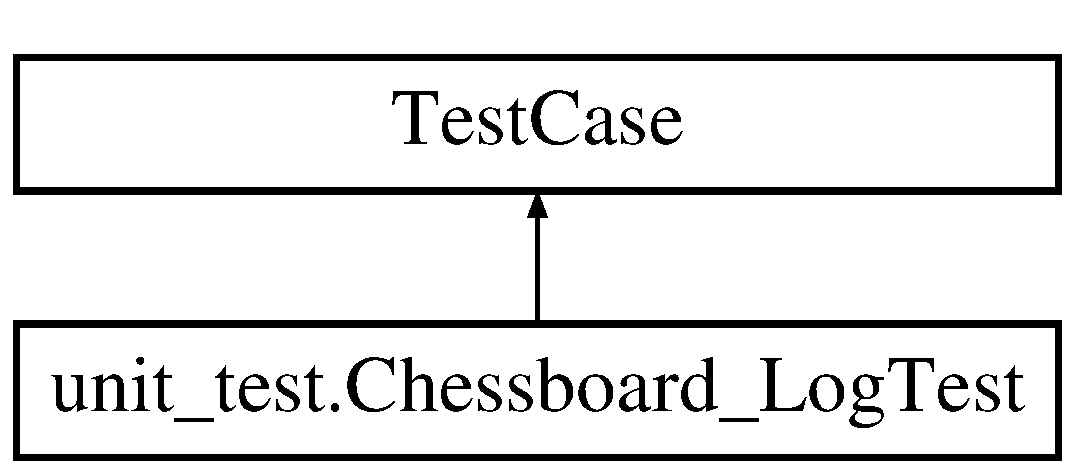
\includegraphics[height=2.000000cm]{classunit__test_1_1_chessboard___log_test}
\end{center}
\end{figure}
\subsection*{Public Member Functions}
\begin{DoxyCompactItemize}
\item 
void \hyperlink{classunit__test_1_1_chessboard___log_test_ac9dd12ea618cdc41706edf1bcaa21937}{test\+To\+Chessboard} ()  throws Exception 
\item 
void \hyperlink{classunit__test_1_1_chessboard___log_test_ab4583090876faf4e112b040acea9e6c1}{test\+Undo} ()  throws Exception 
\end{DoxyCompactItemize}


\subsection{Member Function Documentation}
\hypertarget{classunit__test_1_1_chessboard___log_test_ac9dd12ea618cdc41706edf1bcaa21937}{}\index{unit\+\_\+test\+::\+Chessboard\+\_\+\+Log\+Test@{unit\+\_\+test\+::\+Chessboard\+\_\+\+Log\+Test}!test\+To\+Chessboard@{test\+To\+Chessboard}}
\index{test\+To\+Chessboard@{test\+To\+Chessboard}!unit\+\_\+test\+::\+Chessboard\+\_\+\+Log\+Test@{unit\+\_\+test\+::\+Chessboard\+\_\+\+Log\+Test}}
\subsubsection[{test\+To\+Chessboard}]{\setlength{\rightskip}{0pt plus 5cm}void unit\+\_\+test.\+Chessboard\+\_\+\+Log\+Test.\+test\+To\+Chessboard (
\begin{DoxyParamCaption}
{}
\end{DoxyParamCaption}
) throws Exception\hspace{0.3cm}{\ttfamily [inline]}}\label{classunit__test_1_1_chessboard___log_test_ac9dd12ea618cdc41706edf1bcaa21937}
Test Chessboard Log The chessboard log should have the same content as Chessboard 
\begin{DoxyExceptions}{Exceptions}
{\em Exception} & \\
\hline
\end{DoxyExceptions}
\hypertarget{classunit__test_1_1_chessboard___log_test_ab4583090876faf4e112b040acea9e6c1}{}\index{unit\+\_\+test\+::\+Chessboard\+\_\+\+Log\+Test@{unit\+\_\+test\+::\+Chessboard\+\_\+\+Log\+Test}!test\+Undo@{test\+Undo}}
\index{test\+Undo@{test\+Undo}!unit\+\_\+test\+::\+Chessboard\+\_\+\+Log\+Test@{unit\+\_\+test\+::\+Chessboard\+\_\+\+Log\+Test}}
\subsubsection[{test\+Undo}]{\setlength{\rightskip}{0pt plus 5cm}void unit\+\_\+test.\+Chessboard\+\_\+\+Log\+Test.\+test\+Undo (
\begin{DoxyParamCaption}
{}
\end{DoxyParamCaption}
) throws Exception\hspace{0.3cm}{\ttfamily [inline]}}\label{classunit__test_1_1_chessboard___log_test_ab4583090876faf4e112b040acea9e6c1}
Test undo 
\begin{DoxyExceptions}{Exceptions}
{\em Exception} & \\
\hline
\end{DoxyExceptions}


The documentation for this class was generated from the following file\+:\begin{DoxyCompactItemize}
\item 
src/unit\+\_\+test/Chessboard\+\_\+\+Log\+Test.\+java\end{DoxyCompactItemize}

\hypertarget{classchess_1_1_chessboard___view}{}\section{chess.\+Chessboard\+\_\+\+View Class Reference}
\label{classchess_1_1_chessboard___view}\index{chess.\+Chessboard\+\_\+\+View@{chess.\+Chessboard\+\_\+\+View}}
Inheritance diagram for chess.\+Chessboard\+\_\+\+View\+:\begin{figure}[H]
\begin{center}
\leavevmode
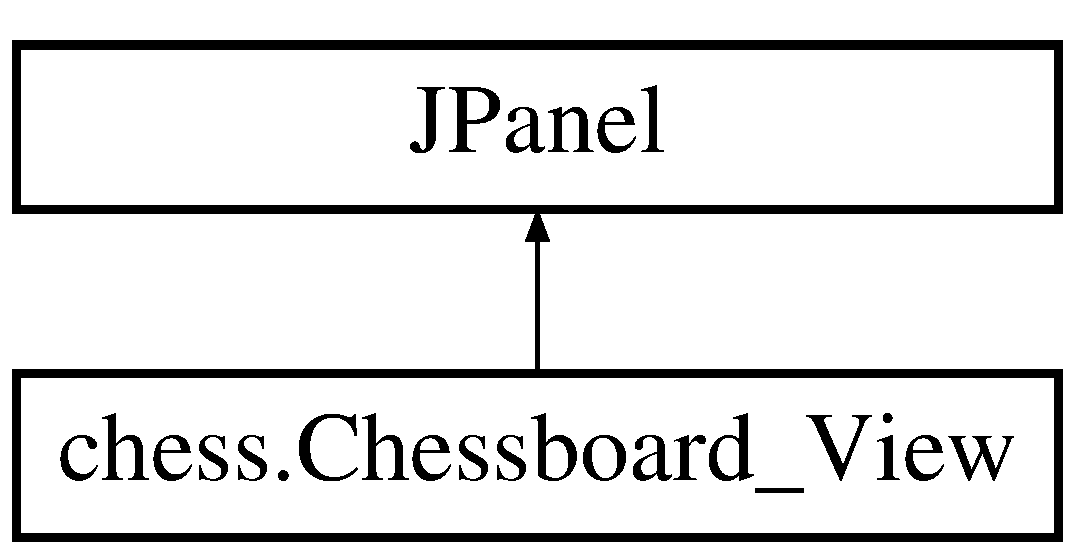
\includegraphics[height=2.000000cm]{classchess_1_1_chessboard___view}
\end{center}
\end{figure}
\subsection*{Public Member Functions}
\begin{DoxyCompactItemize}
\item 
\hyperlink{classchess_1_1_chessboard___view_a603a5829216277fc2987cae53e7cfff0}{Chessboard\+\_\+\+View} (\hyperlink{classchessboard_1_1_chess_board}{Chess\+Board} board, \hyperlink{classchess_1_1_game_controller}{Game\+Controller} game\+\_\+controller, int tile\+\_\+size, int board\+\_\+width, int board\+\_\+height)
\item 
void \hyperlink{classchess_1_1_chessboard___view_a5e73e6ae6724334ae54ac3b5e9969f1f}{paint} (Graphics g)
\item 
void \hyperlink{classchess_1_1_chessboard___view_a0d2cefaddf8ae8a0b52f71347e4017fa}{draw\+Tile\+For\+Board} (Graphics2\+D g2d, int x, int y, Color color)
\item 
void \hyperlink{classchess_1_1_chessboard___view_a1aacffbd1910181a835308ae40afbb0d}{draw\+Piece} (Graphics2\+D g2d, \hyperlink{classpiece_1_1_piece}{Piece} p)
\item 
void \hyperlink{classchess_1_1_chessboard___view_a0e84f18e7cfa470edac2a16e54f7e6eb}{draw\+Possible\+Moves\+For\+Piece} (Graphics2\+D g2d, Array\+List$<$ \hyperlink{classpiece_1_1_coordinate}{Coordinate} $>$ coords)
\item 
void \hyperlink{classchess_1_1_chessboard___view_a43e435d12ccea60a92d3b9d4638d48c3}{draw\+Board} (Graphics2\+D g2d, double clicked\+\_\+x\+\_\+coord, double clicked\+\_\+y\+\_\+coord)
\end{DoxyCompactItemize}
\subsection*{Protected Attributes}
\begin{DoxyCompactItemize}
\item 
\hypertarget{classchess_1_1_chessboard___view_a9672d977ec1b62b2d9f4a47035c8132a}{}\hyperlink{classchessboard_1_1_chess_board}{Chess\+Board} {\bfseries board}\label{classchess_1_1_chessboard___view_a9672d977ec1b62b2d9f4a47035c8132a}

\item 
\hypertarget{classchess_1_1_chessboard___view_aa4fc1ec2f50b04614b0a7fe23a49d6dd}{}int {\bfseries tile\+\_\+size}\label{classchess_1_1_chessboard___view_aa4fc1ec2f50b04614b0a7fe23a49d6dd}

\item 
\hypertarget{classchess_1_1_chessboard___view_ad23b8076d6da9841122d29cca79a99c8}{}\hyperlink{classchess_1_1_game_controller}{Game\+Controller} {\bfseries game\+\_\+controller}\label{classchess_1_1_chessboard___view_ad23b8076d6da9841122d29cca79a99c8}

\item 
\hypertarget{classchess_1_1_chessboard___view_a37099dff3f03c778c3ba348e4cd46536}{}double {\bfseries clicked\+\_\+x\+\_\+coord} = -\/1\label{classchess_1_1_chessboard___view_a37099dff3f03c778c3ba348e4cd46536}

\item 
\hypertarget{classchess_1_1_chessboard___view_a25bc9c5c75ed9926655598a6cd0eced7}{}double {\bfseries clicked\+\_\+y\+\_\+coord} = -\/1\label{classchess_1_1_chessboard___view_a25bc9c5c75ed9926655598a6cd0eced7}

\end{DoxyCompactItemize}


\subsection{Detailed Description}
Chessboard View class This class is used to draw chessboard 

\subsection{Constructor \& Destructor Documentation}
\hypertarget{classchess_1_1_chessboard___view_a603a5829216277fc2987cae53e7cfff0}{}\index{chess\+::\+Chessboard\+\_\+\+View@{chess\+::\+Chessboard\+\_\+\+View}!Chessboard\+\_\+\+View@{Chessboard\+\_\+\+View}}
\index{Chessboard\+\_\+\+View@{Chessboard\+\_\+\+View}!chess\+::\+Chessboard\+\_\+\+View@{chess\+::\+Chessboard\+\_\+\+View}}
\subsubsection[{Chessboard\+\_\+\+View}]{\setlength{\rightskip}{0pt plus 5cm}chess.\+Chessboard\+\_\+\+View.\+Chessboard\+\_\+\+View (
\begin{DoxyParamCaption}
\item[{{\bf Chess\+Board}}]{board, }
\item[{{\bf Game\+Controller}}]{game\+\_\+controller, }
\item[{int}]{tile\+\_\+size, }
\item[{int}]{board\+\_\+width, }
\item[{int}]{board\+\_\+height}
\end{DoxyParamCaption}
)\hspace{0.3cm}{\ttfamily [inline]}}\label{classchess_1_1_chessboard___view_a603a5829216277fc2987cae53e7cfff0}
Mouse press event

\subsection{Member Function Documentation}
\hypertarget{classchess_1_1_chessboard___view_a43e435d12ccea60a92d3b9d4638d48c3}{}\index{chess\+::\+Chessboard\+\_\+\+View@{chess\+::\+Chessboard\+\_\+\+View}!draw\+Board@{draw\+Board}}
\index{draw\+Board@{draw\+Board}!chess\+::\+Chessboard\+\_\+\+View@{chess\+::\+Chessboard\+\_\+\+View}}
\subsubsection[{draw\+Board}]{\setlength{\rightskip}{0pt plus 5cm}void chess.\+Chessboard\+\_\+\+View.\+draw\+Board (
\begin{DoxyParamCaption}
\item[{Graphics2\+D}]{g2d, }
\item[{double}]{clicked\+\_\+x\+\_\+coord, }
\item[{double}]{clicked\+\_\+y\+\_\+coord}
\end{DoxyParamCaption}
)\hspace{0.3cm}{\ttfamily [inline]}}\label{classchess_1_1_chessboard___view_a43e435d12ccea60a92d3b9d4638d48c3}
Draw current chessboard


\begin{DoxyParams}{Parameters}
{\em g2d} & \\
\hline
{\em clicked\+\_\+x\+\_\+coord} & the x coordinate where we clicked \\
\hline
{\em clicked\+\_\+y\+\_\+coord} & the y coordinate where we clicked \\
\hline
\end{DoxyParams}
\hypertarget{classchess_1_1_chessboard___view_a1aacffbd1910181a835308ae40afbb0d}{}\index{chess\+::\+Chessboard\+\_\+\+View@{chess\+::\+Chessboard\+\_\+\+View}!draw\+Piece@{draw\+Piece}}
\index{draw\+Piece@{draw\+Piece}!chess\+::\+Chessboard\+\_\+\+View@{chess\+::\+Chessboard\+\_\+\+View}}
\subsubsection[{draw\+Piece}]{\setlength{\rightskip}{0pt plus 5cm}void chess.\+Chessboard\+\_\+\+View.\+draw\+Piece (
\begin{DoxyParamCaption}
\item[{Graphics2\+D}]{g2d, }
\item[{{\bf Piece}}]{p}
\end{DoxyParamCaption}
)\hspace{0.3cm}{\ttfamily [inline]}}\label{classchess_1_1_chessboard___view_a1aacffbd1910181a835308ae40afbb0d}
Draw Piece on Chessboard 
\begin{DoxyParams}{Parameters}
{\em g2d} & \\
\hline
{\em p} & the piece we want to draw \\
\hline
\end{DoxyParams}
\hypertarget{classchess_1_1_chessboard___view_a0e84f18e7cfa470edac2a16e54f7e6eb}{}\index{chess\+::\+Chessboard\+\_\+\+View@{chess\+::\+Chessboard\+\_\+\+View}!draw\+Possible\+Moves\+For\+Piece@{draw\+Possible\+Moves\+For\+Piece}}
\index{draw\+Possible\+Moves\+For\+Piece@{draw\+Possible\+Moves\+For\+Piece}!chess\+::\+Chessboard\+\_\+\+View@{chess\+::\+Chessboard\+\_\+\+View}}
\subsubsection[{draw\+Possible\+Moves\+For\+Piece}]{\setlength{\rightskip}{0pt plus 5cm}void chess.\+Chessboard\+\_\+\+View.\+draw\+Possible\+Moves\+For\+Piece (
\begin{DoxyParamCaption}
\item[{Graphics2\+D}]{g2d, }
\item[{Array\+List$<$ {\bf Coordinate} $>$}]{coords}
\end{DoxyParamCaption}
)\hspace{0.3cm}{\ttfamily [inline]}}\label{classchess_1_1_chessboard___view_a0e84f18e7cfa470edac2a16e54f7e6eb}
Draw tiles that the piece can move to 
\begin{DoxyParams}{Parameters}
{\em g2d} & \\
\hline
\end{DoxyParams}
\hypertarget{classchess_1_1_chessboard___view_a0d2cefaddf8ae8a0b52f71347e4017fa}{}\index{chess\+::\+Chessboard\+\_\+\+View@{chess\+::\+Chessboard\+\_\+\+View}!draw\+Tile\+For\+Board@{draw\+Tile\+For\+Board}}
\index{draw\+Tile\+For\+Board@{draw\+Tile\+For\+Board}!chess\+::\+Chessboard\+\_\+\+View@{chess\+::\+Chessboard\+\_\+\+View}}
\subsubsection[{draw\+Tile\+For\+Board}]{\setlength{\rightskip}{0pt plus 5cm}void chess.\+Chessboard\+\_\+\+View.\+draw\+Tile\+For\+Board (
\begin{DoxyParamCaption}
\item[{Graphics2\+D}]{g2d, }
\item[{int}]{x, }
\item[{int}]{y, }
\item[{Color}]{color}
\end{DoxyParamCaption}
)\hspace{0.3cm}{\ttfamily [inline]}}\label{classchess_1_1_chessboard___view_a0d2cefaddf8ae8a0b52f71347e4017fa}
Draw tile on board. \begin{DoxyVerb} Coordinate System
 (0, 0) -----------------------> x
 |
 |
 |
 |      canvas coordinate system.
 |     (x, y)
 |
 y
\end{DoxyVerb}



\begin{DoxyParams}{Parameters}
{\em g2d} & \\
\hline
{\em x} & the x coordinate \\
\hline
{\em y} & the y coordinate \\
\hline
{\em color} & the color to draw \\
\hline
\end{DoxyParams}
\hypertarget{classchess_1_1_chessboard___view_a5e73e6ae6724334ae54ac3b5e9969f1f}{}\index{chess\+::\+Chessboard\+\_\+\+View@{chess\+::\+Chessboard\+\_\+\+View}!paint@{paint}}
\index{paint@{paint}!chess\+::\+Chessboard\+\_\+\+View@{chess\+::\+Chessboard\+\_\+\+View}}
\subsubsection[{paint}]{\setlength{\rightskip}{0pt plus 5cm}void chess.\+Chessboard\+\_\+\+View.\+paint (
\begin{DoxyParamCaption}
\item[{Graphics}]{g}
\end{DoxyParamCaption}
)\hspace{0.3cm}{\ttfamily [inline]}}\label{classchess_1_1_chessboard___view_a5e73e6ae6724334ae54ac3b5e9969f1f}
Draw images on canvas 
\begin{DoxyParams}{Parameters}
{\em g} & \\
\hline
\end{DoxyParams}


The documentation for this class was generated from the following file\+:\begin{DoxyCompactItemize}
\item 
src/chess/Chessboard\+\_\+\+View.\+java\end{DoxyCompactItemize}

\hypertarget{classunit__test_1_1_chess_board_test}{}\section{unit\+\_\+test.\+Chess\+Board\+Test Class Reference}
\label{classunit__test_1_1_chess_board_test}\index{unit\+\_\+test.\+Chess\+Board\+Test@{unit\+\_\+test.\+Chess\+Board\+Test}}
\subsection*{Public Member Functions}
\begin{DoxyCompactItemize}
\item 
void \hyperlink{classunit__test_1_1_chess_board_test_a7a0ca34736989173bc4eb60785f5db63}{test\+Is\+Suicide\+Move} ()  throws Exception 
\item 
\hypertarget{classunit__test_1_1_chess_board_test_a07848955e0b2068a8827ec73e2c7f2d5}{}void {\bfseries test\+Player\+Cannot\+Move} ()  throws Exception \label{classunit__test_1_1_chess_board_test_a07848955e0b2068a8827ec73e2c7f2d5}

\item 
void \hyperlink{classunit__test_1_1_chess_board_test_a06ab8a09f928be5c932add8137870e6b}{test\+Is\+Stalemate} ()  throws Exception 
\end{DoxyCompactItemize}


\subsection{Member Function Documentation}
\hypertarget{classunit__test_1_1_chess_board_test_a06ab8a09f928be5c932add8137870e6b}{}\index{unit\+\_\+test\+::\+Chess\+Board\+Test@{unit\+\_\+test\+::\+Chess\+Board\+Test}!test\+Is\+Stalemate@{test\+Is\+Stalemate}}
\index{test\+Is\+Stalemate@{test\+Is\+Stalemate}!unit\+\_\+test\+::\+Chess\+Board\+Test@{unit\+\_\+test\+::\+Chess\+Board\+Test}}
\subsubsection[{test\+Is\+Stalemate}]{\setlength{\rightskip}{0pt plus 5cm}void unit\+\_\+test.\+Chess\+Board\+Test.\+test\+Is\+Stalemate (
\begin{DoxyParamCaption}
{}
\end{DoxyParamCaption}
) throws Exception\hspace{0.3cm}{\ttfamily [inline]}}\label{classunit__test_1_1_chess_board_test_a06ab8a09f928be5c932add8137870e6b}
test the judgement of stalemate 
\begin{DoxyExceptions}{Exceptions}
{\em Exception} & \\
\hline
\end{DoxyExceptions}
\hypertarget{classunit__test_1_1_chess_board_test_a7a0ca34736989173bc4eb60785f5db63}{}\index{unit\+\_\+test\+::\+Chess\+Board\+Test@{unit\+\_\+test\+::\+Chess\+Board\+Test}!test\+Is\+Suicide\+Move@{test\+Is\+Suicide\+Move}}
\index{test\+Is\+Suicide\+Move@{test\+Is\+Suicide\+Move}!unit\+\_\+test\+::\+Chess\+Board\+Test@{unit\+\_\+test\+::\+Chess\+Board\+Test}}
\subsubsection[{test\+Is\+Suicide\+Move}]{\setlength{\rightskip}{0pt plus 5cm}void unit\+\_\+test.\+Chess\+Board\+Test.\+test\+Is\+Suicide\+Move (
\begin{DoxyParamCaption}
{}
\end{DoxyParamCaption}
) throws Exception\hspace{0.3cm}{\ttfamily [inline]}}\label{classunit__test_1_1_chess_board_test_a7a0ca34736989173bc4eb60785f5db63}
Test the judgement of suicide move 
\begin{DoxyExceptions}{Exceptions}
{\em Exception} & \\
\hline
\end{DoxyExceptions}


The documentation for this class was generated from the following file\+:\begin{DoxyCompactItemize}
\item 
src/unit\+\_\+test/Chess\+Board\+Test.\+java\end{DoxyCompactItemize}

\hypertarget{classpiece_1_1_coordinate}{}\section{piece.\+Coordinate Class Reference}
\label{classpiece_1_1_coordinate}\index{piece.\+Coordinate@{piece.\+Coordinate}}
\subsection*{Public Member Functions}
\begin{DoxyCompactItemize}
\item 
\hyperlink{classpiece_1_1_coordinate_aceef65dd72d3033c0c6e9a9242f64dab}{Coordinate} ()
\item 
\hyperlink{classpiece_1_1_coordinate_a5255d45526652ad0295c1f96d2d0ee0d}{Coordinate} (int x, int y)
\item 
int \hyperlink{classpiece_1_1_coordinate_a7acda6e728ca9ef57676e0c690ecd1cc}{get\+X} ()
\item 
void \hyperlink{classpiece_1_1_coordinate_a46f6fd2af39862f0e2a049079ace93ae}{set\+X} (int x)
\item 
int \hyperlink{classpiece_1_1_coordinate_a49cce3c806c30d970f9d9b605100dd9e}{get\+Y} ()
\item 
void \hyperlink{classpiece_1_1_coordinate_a25033858f5498bda280f8226dbcb5a4f}{set\+Y} (int y)
\end{DoxyCompactItemize}


\subsection{Detailed Description}
Created by wangyiyi on 2/12/15.

\hyperlink{classpiece_1_1_coordinate}{Coordinate} Class This class is used to store x, y coordinate for \hyperlink{classpiece_1_1_piece}{Piece} 

\subsection{Constructor \& Destructor Documentation}
\hypertarget{classpiece_1_1_coordinate_aceef65dd72d3033c0c6e9a9242f64dab}{}\index{piece\+::\+Coordinate@{piece\+::\+Coordinate}!Coordinate@{Coordinate}}
\index{Coordinate@{Coordinate}!piece\+::\+Coordinate@{piece\+::\+Coordinate}}
\subsubsection[{Coordinate}]{\setlength{\rightskip}{0pt plus 5cm}piece.\+Coordinate.\+Coordinate (
\begin{DoxyParamCaption}
{}
\end{DoxyParamCaption}
)\hspace{0.3cm}{\ttfamily [inline]}}\label{classpiece_1_1_coordinate_aceef65dd72d3033c0c6e9a9242f64dab}
Constructor\+: set default x = y = -\/1 \hypertarget{classpiece_1_1_coordinate_a5255d45526652ad0295c1f96d2d0ee0d}{}\index{piece\+::\+Coordinate@{piece\+::\+Coordinate}!Coordinate@{Coordinate}}
\index{Coordinate@{Coordinate}!piece\+::\+Coordinate@{piece\+::\+Coordinate}}
\subsubsection[{Coordinate}]{\setlength{\rightskip}{0pt plus 5cm}piece.\+Coordinate.\+Coordinate (
\begin{DoxyParamCaption}
\item[{int}]{x, }
\item[{int}]{y}
\end{DoxyParamCaption}
)\hspace{0.3cm}{\ttfamily [inline]}}\label{classpiece_1_1_coordinate_a5255d45526652ad0295c1f96d2d0ee0d}
Constructor\+: set x and y 
\begin{DoxyParams}{Parameters}
{\em x} & the x coordinate \\
\hline
{\em y} & the y coordinate \\
\hline
\end{DoxyParams}


\subsection{Member Function Documentation}
\hypertarget{classpiece_1_1_coordinate_a7acda6e728ca9ef57676e0c690ecd1cc}{}\index{piece\+::\+Coordinate@{piece\+::\+Coordinate}!get\+X@{get\+X}}
\index{get\+X@{get\+X}!piece\+::\+Coordinate@{piece\+::\+Coordinate}}
\subsubsection[{get\+X}]{\setlength{\rightskip}{0pt plus 5cm}int piece.\+Coordinate.\+get\+X (
\begin{DoxyParamCaption}
{}
\end{DoxyParamCaption}
)\hspace{0.3cm}{\ttfamily [inline]}}\label{classpiece_1_1_coordinate_a7acda6e728ca9ef57676e0c690ecd1cc}
Getter, return x \begin{DoxyReturn}{Returns}
the x coordinate 
\end{DoxyReturn}
\hypertarget{classpiece_1_1_coordinate_a49cce3c806c30d970f9d9b605100dd9e}{}\index{piece\+::\+Coordinate@{piece\+::\+Coordinate}!get\+Y@{get\+Y}}
\index{get\+Y@{get\+Y}!piece\+::\+Coordinate@{piece\+::\+Coordinate}}
\subsubsection[{get\+Y}]{\setlength{\rightskip}{0pt plus 5cm}int piece.\+Coordinate.\+get\+Y (
\begin{DoxyParamCaption}
{}
\end{DoxyParamCaption}
)\hspace{0.3cm}{\ttfamily [inline]}}\label{classpiece_1_1_coordinate_a49cce3c806c30d970f9d9b605100dd9e}
Getter, return Y \begin{DoxyReturn}{Returns}
the y coordinate 
\end{DoxyReturn}
\hypertarget{classpiece_1_1_coordinate_a46f6fd2af39862f0e2a049079ace93ae}{}\index{piece\+::\+Coordinate@{piece\+::\+Coordinate}!set\+X@{set\+X}}
\index{set\+X@{set\+X}!piece\+::\+Coordinate@{piece\+::\+Coordinate}}
\subsubsection[{set\+X}]{\setlength{\rightskip}{0pt plus 5cm}void piece.\+Coordinate.\+set\+X (
\begin{DoxyParamCaption}
\item[{int}]{x}
\end{DoxyParamCaption}
)\hspace{0.3cm}{\ttfamily [inline]}}\label{classpiece_1_1_coordinate_a46f6fd2af39862f0e2a049079ace93ae}
Setter, set x 
\begin{DoxyParams}{Parameters}
{\em x} & set value \\
\hline
\end{DoxyParams}
\hypertarget{classpiece_1_1_coordinate_a25033858f5498bda280f8226dbcb5a4f}{}\index{piece\+::\+Coordinate@{piece\+::\+Coordinate}!set\+Y@{set\+Y}}
\index{set\+Y@{set\+Y}!piece\+::\+Coordinate@{piece\+::\+Coordinate}}
\subsubsection[{set\+Y}]{\setlength{\rightskip}{0pt plus 5cm}void piece.\+Coordinate.\+set\+Y (
\begin{DoxyParamCaption}
\item[{int}]{y}
\end{DoxyParamCaption}
)\hspace{0.3cm}{\ttfamily [inline]}}\label{classpiece_1_1_coordinate_a25033858f5498bda280f8226dbcb5a4f}
Setter, set Y 
\begin{DoxyParams}{Parameters}
{\em y} & set value \\
\hline
\end{DoxyParams}


The documentation for this class was generated from the following file\+:\begin{DoxyCompactItemize}
\item 
src/piece/Coordinate.\+java\end{DoxyCompactItemize}

\hypertarget{classchess_1_1_game}{}\section{chess.\+Game Class Reference}
\label{classchess_1_1_game}\index{chess.\+Game@{chess.\+Game}}
\subsection*{Public Member Functions}
\begin{DoxyCompactItemize}
\item 
\hyperlink{classchess_1_1_game_a1027946d6b89410913542ffefde89048}{Game} (\hyperlink{classchessboard_1_1_chess_board}{Chess\+Board} board, \hyperlink{classchess_1_1_game_controller}{Game\+Controller} game\+\_\+controller, \hyperlink{classchess_1_1_game_view}{Game\+View} game\+\_\+view)
\item 
\hypertarget{classchess_1_1_game_a62625ed6fdf31f366b4d9fa7b057ce11}{}void {\bfseries start\+Game} ()\label{classchess_1_1_game_a62625ed6fdf31f366b4d9fa7b057ce11}

\end{DoxyCompactItemize}
\subsection*{Static Public Member Functions}
\begin{DoxyCompactItemize}
\item 
static void \hyperlink{classchess_1_1_game_a26b35a6e1a16f410fa2182794ffce9ae}{main} (String\mbox{[}$\,$\mbox{]} args)
\end{DoxyCompactItemize}


\subsection{Detailed Description}
Main \hyperlink{classchess_1_1_game}{Game} 

\subsection{Constructor \& Destructor Documentation}
\hypertarget{classchess_1_1_game_a1027946d6b89410913542ffefde89048}{}\index{chess\+::\+Game@{chess\+::\+Game}!Game@{Game}}
\index{Game@{Game}!chess\+::\+Game@{chess\+::\+Game}}
\subsubsection[{Game}]{\setlength{\rightskip}{0pt plus 5cm}chess.\+Game.\+Game (
\begin{DoxyParamCaption}
\item[{{\bf Chess\+Board}}]{board, }
\item[{{\bf Game\+Controller}}]{game\+\_\+controller, }
\item[{{\bf Game\+View}}]{game\+\_\+view}
\end{DoxyParamCaption}
)\hspace{0.3cm}{\ttfamily [inline]}}\label{classchess_1_1_game_a1027946d6b89410913542ffefde89048}
Constructor\+: init game, set necessary properties. 
\begin{DoxyParams}{Parameters}
{\em board} & \\
\hline
{\em game\+\_\+controller} & \\
\hline
{\em game\+\_\+view} & \\
\hline
\end{DoxyParams}


\subsection{Member Function Documentation}
\hypertarget{classchess_1_1_game_a26b35a6e1a16f410fa2182794ffce9ae}{}\index{chess\+::\+Game@{chess\+::\+Game}!main@{main}}
\index{main@{main}!chess\+::\+Game@{chess\+::\+Game}}
\subsubsection[{main}]{\setlength{\rightskip}{0pt plus 5cm}static void chess.\+Game.\+main (
\begin{DoxyParamCaption}
\item[{String\mbox{[}$\,$\mbox{]}}]{args}
\end{DoxyParamCaption}
)\hspace{0.3cm}{\ttfamily [inline]}, {\ttfamily [static]}}\label{classchess_1_1_game_a26b35a6e1a16f410fa2182794ffce9ae}
Main function 
\begin{DoxyParams}{Parameters}
{\em args} & \\
\hline
\end{DoxyParams}


The documentation for this class was generated from the following file\+:\begin{DoxyCompactItemize}
\item 
src/chess/Game.\+java\end{DoxyCompactItemize}

\hypertarget{classchess_1_1_game_controller}{}\section{chess.\+Game\+Controller Class Reference}
\label{classchess_1_1_game_controller}\index{chess.\+Game\+Controller@{chess.\+Game\+Controller}}
\subsection*{Public Member Functions}
\begin{DoxyCompactItemize}
\item 
\hyperlink{classchess_1_1_game_controller_a807721753fe9883b7573eee34f3c8614}{Game\+Controller} (\hyperlink{classchessboard_1_1_chess_board}{Chess\+Board} board, \hyperlink{classchess_1_1_game_view}{Game\+View} game\+\_\+view)
\item 
boolean \hyperlink{classchess_1_1_game_controller_ae38db155ab79e9c899405de2116c6991}{players\+King\+Is\+In\+Check} (\hyperlink{enumchessboard_1_1_player}{Player} player)
\item 
String \hyperlink{classchess_1_1_game_controller_ac6c59b1167b78b3963c7ecdb53f3541b}{is\+Checkmate\+Or\+Stalemate} ()
\item 
void \hyperlink{classchess_1_1_game_controller_abecbe39ba58ba9547d3bdb7c238ef348}{game\+Is\+Over} (String status)
\item 
void \hyperlink{classchess_1_1_game_controller_a7d11340cfe1ebe2af49b5108fcaedd18}{move\+Piece\+To\+Opponent\+Piece\+Location\+If\+Valid} (J\+Panel panel, \hyperlink{classpiece_1_1_piece}{Piece} opponent\+\_\+piece)
\item 
void \hyperlink{classchess_1_1_game_controller_a9305375980a713c74e6515c16ebefbbc}{move\+Player\+Piece\+To\+Empty\+Tile\+If\+Valid} (J\+Panel panel, int x, int y)
\item 
\hyperlink{enumchessboard_1_1_player}{Player} \hyperlink{classchess_1_1_game_controller_a47ff441aae36d704a7a9c9315d61e284}{get\+Player\+For\+This\+Turn} ()
\item 
void \hyperlink{classchess_1_1_game_controller_a978f68fb8834594117aa49b03dbdcf3d}{check\+User\+Click} (Graphics2\+D g2d, double clicked\+\_\+x\+\_\+coord, double clicked\+\_\+y\+\_\+coord)
\item 
void \hyperlink{classchess_1_1_game_controller_af6003c4092b5c51ab7e4e9b064823bfc}{update\+Message} (String message)
\item 
void \hyperlink{classchess_1_1_game_controller_a1922c179d1cf4b115e68a79089f03faa}{start\+New\+Game} (int game\+\_\+mode)
\item 
void \hyperlink{classchess_1_1_game_controller_a152dd59c8605ceab2b0ca60097097f5e}{clicked\+Start\+Button} ()
\item 
void \hyperlink{classchess_1_1_game_controller_a22800c136daed1f9208be17e1c8b9c64}{clicked\+Restart\+Button} ()
\item 
void \hyperlink{classchess_1_1_game_controller_a76b4903a383e6b16e4cd8ad85dbeda90}{clicked\+Forfeit\+Button} ()
\item 
void \hyperlink{classchess_1_1_game_controller_ae179437fea74f6aa6ce03efd8b786b12}{clicked\+Undo\+Button} ()
\item 
void \hyperlink{classchess_1_1_game_controller_aa74fdd8304cba081746e040df2a2a4bb}{update\+Player\+Name} (J\+Button btn)
\end{DoxyCompactItemize}
\subsection*{Protected Attributes}
\begin{DoxyCompactItemize}
\item 
\hypertarget{classchess_1_1_game_controller_a610e87d934d993ee057760c0460cc684}{}\hyperlink{classchessboard_1_1_chess_board}{Chess\+Board} {\bfseries board}\label{classchess_1_1_game_controller_a610e87d934d993ee057760c0460cc684}

\item 
\hypertarget{classchess_1_1_game_controller_aa1e8ed0fa618f886c88b301188bba6a2}{}\hyperlink{classchess_1_1_game_view}{Game\+View} {\bfseries game\+\_\+view}\label{classchess_1_1_game_controller_aa1e8ed0fa618f886c88b301188bba6a2}

\item 
\hypertarget{classchess_1_1_game_controller_a09e8ba553128ea3e3074416f086bdb98}{}\hyperlink{classpiece_1_1_piece}{Piece} {\bfseries chosen\+\_\+piece}\label{classchess_1_1_game_controller_a09e8ba553128ea3e3074416f086bdb98}

\item 
\hypertarget{classchess_1_1_game_controller_a8f873f2f1566ac39dbcced78a26c4761}{}boolean {\bfseries game\+\_\+start}\label{classchess_1_1_game_controller_a8f873f2f1566ac39dbcced78a26c4761}

\item 
\hypertarget{classchess_1_1_game_controller_a41abf03bb07369cde27f1fc1fd49e09d}{}String {\bfseries player1\+\_\+name}\label{classchess_1_1_game_controller_a41abf03bb07369cde27f1fc1fd49e09d}

\item 
\hypertarget{classchess_1_1_game_controller_aa98adb033188584d5f6f432671bfbf81}{}String {\bfseries player2\+\_\+name}\label{classchess_1_1_game_controller_aa98adb033188584d5f6f432671bfbf81}

\item 
\hypertarget{classchess_1_1_game_controller_a1caee96ac57ba2cd1382b87ad9c77c4a}{}int {\bfseries player1\+\_\+score}\label{classchess_1_1_game_controller_a1caee96ac57ba2cd1382b87ad9c77c4a}

\item 
\hypertarget{classchess_1_1_game_controller_ae0ff8b75fc4348be262301766505860c}{}int {\bfseries player2\+\_\+score}\label{classchess_1_1_game_controller_ae0ff8b75fc4348be262301766505860c}

\item 
\hypertarget{classchess_1_1_game_controller_a62b849f468a91261ab5a701c8932e36f}{}String {\bfseries message}\label{classchess_1_1_game_controller_a62b849f468a91261ab5a701c8932e36f}

\end{DoxyCompactItemize}


\subsection{Detailed Description}
Created by wangyiyi on 2/25/15. \hyperlink{classchess_1_1_game}{Game} Controller 

\subsection{Constructor \& Destructor Documentation}
\hypertarget{classchess_1_1_game_controller_a807721753fe9883b7573eee34f3c8614}{}\index{chess\+::\+Game\+Controller@{chess\+::\+Game\+Controller}!Game\+Controller@{Game\+Controller}}
\index{Game\+Controller@{Game\+Controller}!chess\+::\+Game\+Controller@{chess\+::\+Game\+Controller}}
\subsubsection[{Game\+Controller}]{\setlength{\rightskip}{0pt plus 5cm}chess.\+Game\+Controller.\+Game\+Controller (
\begin{DoxyParamCaption}
\item[{{\bf Chess\+Board}}]{board, }
\item[{{\bf Game\+View}}]{game\+\_\+view}
\end{DoxyParamCaption}
)\hspace{0.3cm}{\ttfamily [inline]}}\label{classchess_1_1_game_controller_a807721753fe9883b7573eee34f3c8614}
Constructor\+: initialize game controller 
\begin{DoxyParams}{Parameters}
{\em board} & \\
\hline
{\em game\+\_\+view} & \\
\hline
\end{DoxyParams}


\subsection{Member Function Documentation}
\hypertarget{classchess_1_1_game_controller_a978f68fb8834594117aa49b03dbdcf3d}{}\index{chess\+::\+Game\+Controller@{chess\+::\+Game\+Controller}!check\+User\+Click@{check\+User\+Click}}
\index{check\+User\+Click@{check\+User\+Click}!chess\+::\+Game\+Controller@{chess\+::\+Game\+Controller}}
\subsubsection[{check\+User\+Click}]{\setlength{\rightskip}{0pt plus 5cm}void chess.\+Game\+Controller.\+check\+User\+Click (
\begin{DoxyParamCaption}
\item[{Graphics2\+D}]{g2d, }
\item[{double}]{clicked\+\_\+x\+\_\+coord, }
\item[{double}]{clicked\+\_\+y\+\_\+coord}
\end{DoxyParamCaption}
)\hspace{0.3cm}{\ttfamily [inline]}}\label{classchess_1_1_game_controller_a978f68fb8834594117aa49b03dbdcf3d}
Check user mouse click, and update gui. 
\begin{DoxyParams}{Parameters}
{\em g2d} & \\
\hline
{\em clicked\+\_\+x\+\_\+coord} & \\
\hline
{\em clicked\+\_\+y\+\_\+coord} & \\
\hline
\end{DoxyParams}
\hypertarget{classchess_1_1_game_controller_a76b4903a383e6b16e4cd8ad85dbeda90}{}\index{chess\+::\+Game\+Controller@{chess\+::\+Game\+Controller}!clicked\+Forfeit\+Button@{clicked\+Forfeit\+Button}}
\index{clicked\+Forfeit\+Button@{clicked\+Forfeit\+Button}!chess\+::\+Game\+Controller@{chess\+::\+Game\+Controller}}
\subsubsection[{clicked\+Forfeit\+Button}]{\setlength{\rightskip}{0pt plus 5cm}void chess.\+Game\+Controller.\+clicked\+Forfeit\+Button (
\begin{DoxyParamCaption}
{}
\end{DoxyParamCaption}
)\hspace{0.3cm}{\ttfamily [inline]}}\label{classchess_1_1_game_controller_a76b4903a383e6b16e4cd8ad85dbeda90}
Player clicked forfeit button \hypertarget{classchess_1_1_game_controller_a22800c136daed1f9208be17e1c8b9c64}{}\index{chess\+::\+Game\+Controller@{chess\+::\+Game\+Controller}!clicked\+Restart\+Button@{clicked\+Restart\+Button}}
\index{clicked\+Restart\+Button@{clicked\+Restart\+Button}!chess\+::\+Game\+Controller@{chess\+::\+Game\+Controller}}
\subsubsection[{clicked\+Restart\+Button}]{\setlength{\rightskip}{0pt plus 5cm}void chess.\+Game\+Controller.\+clicked\+Restart\+Button (
\begin{DoxyParamCaption}
{}
\end{DoxyParamCaption}
)\hspace{0.3cm}{\ttfamily [inline]}}\label{classchess_1_1_game_controller_a22800c136daed1f9208be17e1c8b9c64}
Player clicked restart button \hypertarget{classchess_1_1_game_controller_a152dd59c8605ceab2b0ca60097097f5e}{}\index{chess\+::\+Game\+Controller@{chess\+::\+Game\+Controller}!clicked\+Start\+Button@{clicked\+Start\+Button}}
\index{clicked\+Start\+Button@{clicked\+Start\+Button}!chess\+::\+Game\+Controller@{chess\+::\+Game\+Controller}}
\subsubsection[{clicked\+Start\+Button}]{\setlength{\rightskip}{0pt plus 5cm}void chess.\+Game\+Controller.\+clicked\+Start\+Button (
\begin{DoxyParamCaption}
{}
\end{DoxyParamCaption}
)\hspace{0.3cm}{\ttfamily [inline]}}\label{classchess_1_1_game_controller_a152dd59c8605ceab2b0ca60097097f5e}
Player clicked start button \hypertarget{classchess_1_1_game_controller_ae179437fea74f6aa6ce03efd8b786b12}{}\index{chess\+::\+Game\+Controller@{chess\+::\+Game\+Controller}!clicked\+Undo\+Button@{clicked\+Undo\+Button}}
\index{clicked\+Undo\+Button@{clicked\+Undo\+Button}!chess\+::\+Game\+Controller@{chess\+::\+Game\+Controller}}
\subsubsection[{clicked\+Undo\+Button}]{\setlength{\rightskip}{0pt plus 5cm}void chess.\+Game\+Controller.\+clicked\+Undo\+Button (
\begin{DoxyParamCaption}
{}
\end{DoxyParamCaption}
)\hspace{0.3cm}{\ttfamily [inline]}}\label{classchess_1_1_game_controller_ae179437fea74f6aa6ce03efd8b786b12}
Player clicked undo button \hypertarget{classchess_1_1_game_controller_abecbe39ba58ba9547d3bdb7c238ef348}{}\index{chess\+::\+Game\+Controller@{chess\+::\+Game\+Controller}!game\+Is\+Over@{game\+Is\+Over}}
\index{game\+Is\+Over@{game\+Is\+Over}!chess\+::\+Game\+Controller@{chess\+::\+Game\+Controller}}
\subsubsection[{game\+Is\+Over}]{\setlength{\rightskip}{0pt plus 5cm}void chess.\+Game\+Controller.\+game\+Is\+Over (
\begin{DoxyParamCaption}
\item[{String}]{status}
\end{DoxyParamCaption}
)\hspace{0.3cm}{\ttfamily [inline]}}\label{classchess_1_1_game_controller_abecbe39ba58ba9547d3bdb7c238ef348}
\hyperlink{classchess_1_1_game}{Game} is over 
\begin{DoxyParams}{Parameters}
{\em status} & \\
\hline
\end{DoxyParams}
\hypertarget{classchess_1_1_game_controller_a47ff441aae36d704a7a9c9315d61e284}{}\index{chess\+::\+Game\+Controller@{chess\+::\+Game\+Controller}!get\+Player\+For\+This\+Turn@{get\+Player\+For\+This\+Turn}}
\index{get\+Player\+For\+This\+Turn@{get\+Player\+For\+This\+Turn}!chess\+::\+Game\+Controller@{chess\+::\+Game\+Controller}}
\subsubsection[{get\+Player\+For\+This\+Turn}]{\setlength{\rightskip}{0pt plus 5cm}{\bf Player} chess.\+Game\+Controller.\+get\+Player\+For\+This\+Turn (
\begin{DoxyParamCaption}
{}
\end{DoxyParamCaption}
)\hspace{0.3cm}{\ttfamily [inline]}}\label{classchess_1_1_game_controller_a47ff441aae36d704a7a9c9315d61e284}
\begin{DoxyReturn}{Returns}
Player for this turn. 
\end{DoxyReturn}
\hypertarget{classchess_1_1_game_controller_ac6c59b1167b78b3963c7ecdb53f3541b}{}\index{chess\+::\+Game\+Controller@{chess\+::\+Game\+Controller}!is\+Checkmate\+Or\+Stalemate@{is\+Checkmate\+Or\+Stalemate}}
\index{is\+Checkmate\+Or\+Stalemate@{is\+Checkmate\+Or\+Stalemate}!chess\+::\+Game\+Controller@{chess\+::\+Game\+Controller}}
\subsubsection[{is\+Checkmate\+Or\+Stalemate}]{\setlength{\rightskip}{0pt plus 5cm}String chess.\+Game\+Controller.\+is\+Checkmate\+Or\+Stalemate (
\begin{DoxyParamCaption}
{}
\end{DoxyParamCaption}
)\hspace{0.3cm}{\ttfamily [inline]}}\label{classchess_1_1_game_controller_ac6c59b1167b78b3963c7ecdb53f3541b}
check whether is checkmate or stalemate \begin{DoxyReturn}{Returns}
null if neither checkmate nor stalemate; return \char`\"{}checkmate\char`\"{} if checkmate; return \char`\"{}stalemate\char`\"{} if stalemate 
\end{DoxyReturn}
\hypertarget{classchess_1_1_game_controller_a7d11340cfe1ebe2af49b5108fcaedd18}{}\index{chess\+::\+Game\+Controller@{chess\+::\+Game\+Controller}!move\+Piece\+To\+Opponent\+Piece\+Location\+If\+Valid@{move\+Piece\+To\+Opponent\+Piece\+Location\+If\+Valid}}
\index{move\+Piece\+To\+Opponent\+Piece\+Location\+If\+Valid@{move\+Piece\+To\+Opponent\+Piece\+Location\+If\+Valid}!chess\+::\+Game\+Controller@{chess\+::\+Game\+Controller}}
\subsubsection[{move\+Piece\+To\+Opponent\+Piece\+Location\+If\+Valid}]{\setlength{\rightskip}{0pt plus 5cm}void chess.\+Game\+Controller.\+move\+Piece\+To\+Opponent\+Piece\+Location\+If\+Valid (
\begin{DoxyParamCaption}
\item[{J\+Panel}]{panel, }
\item[{{\bf Piece}}]{opponent\+\_\+piece}
\end{DoxyParamCaption}
)\hspace{0.3cm}{\ttfamily [inline]}}\label{classchess_1_1_game_controller_a7d11340cfe1ebe2af49b5108fcaedd18}
Player\textquotesingle{}s piece captures opponent piece

If it can be done, redraw the chessboard; otherwise do nothing 
\begin{DoxyParams}{Parameters}
{\em panel} & \\
\hline
{\em opponent\+\_\+piece} & opponent piece \\
\hline
\end{DoxyParams}
\hypertarget{classchess_1_1_game_controller_a9305375980a713c74e6515c16ebefbbc}{}\index{chess\+::\+Game\+Controller@{chess\+::\+Game\+Controller}!move\+Player\+Piece\+To\+Empty\+Tile\+If\+Valid@{move\+Player\+Piece\+To\+Empty\+Tile\+If\+Valid}}
\index{move\+Player\+Piece\+To\+Empty\+Tile\+If\+Valid@{move\+Player\+Piece\+To\+Empty\+Tile\+If\+Valid}!chess\+::\+Game\+Controller@{chess\+::\+Game\+Controller}}
\subsubsection[{move\+Player\+Piece\+To\+Empty\+Tile\+If\+Valid}]{\setlength{\rightskip}{0pt plus 5cm}void chess.\+Game\+Controller.\+move\+Player\+Piece\+To\+Empty\+Tile\+If\+Valid (
\begin{DoxyParamCaption}
\item[{J\+Panel}]{panel, }
\item[{int}]{x, }
\item[{int}]{y}
\end{DoxyParamCaption}
)\hspace{0.3cm}{\ttfamily [inline]}}\label{classchess_1_1_game_controller_a9305375980a713c74e6515c16ebefbbc}
Move player\textquotesingle{}s piece to unoccupied tile if valid, which means the move is not a suicide move 
\begin{DoxyParams}{Parameters}
{\em panel} & \\
\hline
{\em x} & the x coord to move to \\
\hline
{\em y} & the y coord to move to \\
\hline
\end{DoxyParams}
\hypertarget{classchess_1_1_game_controller_ae38db155ab79e9c899405de2116c6991}{}\index{chess\+::\+Game\+Controller@{chess\+::\+Game\+Controller}!players\+King\+Is\+In\+Check@{players\+King\+Is\+In\+Check}}
\index{players\+King\+Is\+In\+Check@{players\+King\+Is\+In\+Check}!chess\+::\+Game\+Controller@{chess\+::\+Game\+Controller}}
\subsubsection[{players\+King\+Is\+In\+Check}]{\setlength{\rightskip}{0pt plus 5cm}boolean chess.\+Game\+Controller.\+players\+King\+Is\+In\+Check (
\begin{DoxyParamCaption}
\item[{{\bf Player}}]{player}
\end{DoxyParamCaption}
)\hspace{0.3cm}{\ttfamily [inline]}}\label{classchess_1_1_game_controller_ae38db155ab79e9c899405de2116c6991}
Check whether player\textquotesingle{}s king is in check 
\begin{DoxyParams}{Parameters}
{\em player} & check this player\textquotesingle{}s king \\
\hline
\end{DoxyParams}
\begin{DoxyReturn}{Returns}
true if king is in check. 
\end{DoxyReturn}
\hypertarget{classchess_1_1_game_controller_a1922c179d1cf4b115e68a79089f03faa}{}\index{chess\+::\+Game\+Controller@{chess\+::\+Game\+Controller}!start\+New\+Game@{start\+New\+Game}}
\index{start\+New\+Game@{start\+New\+Game}!chess\+::\+Game\+Controller@{chess\+::\+Game\+Controller}}
\subsubsection[{start\+New\+Game}]{\setlength{\rightskip}{0pt plus 5cm}void chess.\+Game\+Controller.\+start\+New\+Game (
\begin{DoxyParamCaption}
\item[{int}]{game\+\_\+mode}
\end{DoxyParamCaption}
)\hspace{0.3cm}{\ttfamily [inline]}}\label{classchess_1_1_game_controller_a1922c179d1cf4b115e68a79089f03faa}
Start a new game if game\+\_\+mode equals 1 =$>$ fantasy mode; otherwise classic mode 
\begin{DoxyParams}{Parameters}
{\em game\+\_\+mode} & \\
\hline
\end{DoxyParams}
\hypertarget{classchess_1_1_game_controller_af6003c4092b5c51ab7e4e9b064823bfc}{}\index{chess\+::\+Game\+Controller@{chess\+::\+Game\+Controller}!update\+Message@{update\+Message}}
\index{update\+Message@{update\+Message}!chess\+::\+Game\+Controller@{chess\+::\+Game\+Controller}}
\subsubsection[{update\+Message}]{\setlength{\rightskip}{0pt plus 5cm}void chess.\+Game\+Controller.\+update\+Message (
\begin{DoxyParamCaption}
\item[{String}]{message}
\end{DoxyParamCaption}
)\hspace{0.3cm}{\ttfamily [inline]}}\label{classchess_1_1_game_controller_af6003c4092b5c51ab7e4e9b064823bfc}
Update game message 
\begin{DoxyParams}{Parameters}
{\em message} & \\
\hline
\end{DoxyParams}
\hypertarget{classchess_1_1_game_controller_aa74fdd8304cba081746e040df2a2a4bb}{}\index{chess\+::\+Game\+Controller@{chess\+::\+Game\+Controller}!update\+Player\+Name@{update\+Player\+Name}}
\index{update\+Player\+Name@{update\+Player\+Name}!chess\+::\+Game\+Controller@{chess\+::\+Game\+Controller}}
\subsubsection[{update\+Player\+Name}]{\setlength{\rightskip}{0pt plus 5cm}void chess.\+Game\+Controller.\+update\+Player\+Name (
\begin{DoxyParamCaption}
\item[{J\+Button}]{btn}
\end{DoxyParamCaption}
)\hspace{0.3cm}{\ttfamily [inline]}}\label{classchess_1_1_game_controller_aa74fdd8304cba081746e040df2a2a4bb}
Update Player Name 
\begin{DoxyParams}{Parameters}
{\em btn} & \\
\hline
\end{DoxyParams}


The documentation for this class was generated from the following file\+:\begin{DoxyCompactItemize}
\item 
src/chess/Game\+Controller.\+java\end{DoxyCompactItemize}

\hypertarget{classchess_1_1_game_view}{}\section{chess.\+Game\+View Class Reference}
\label{classchess_1_1_game_view}\index{chess.\+Game\+View@{chess.\+Game\+View}}
Inheritance diagram for chess.\+Game\+View\+:\begin{figure}[H]
\begin{center}
\leavevmode
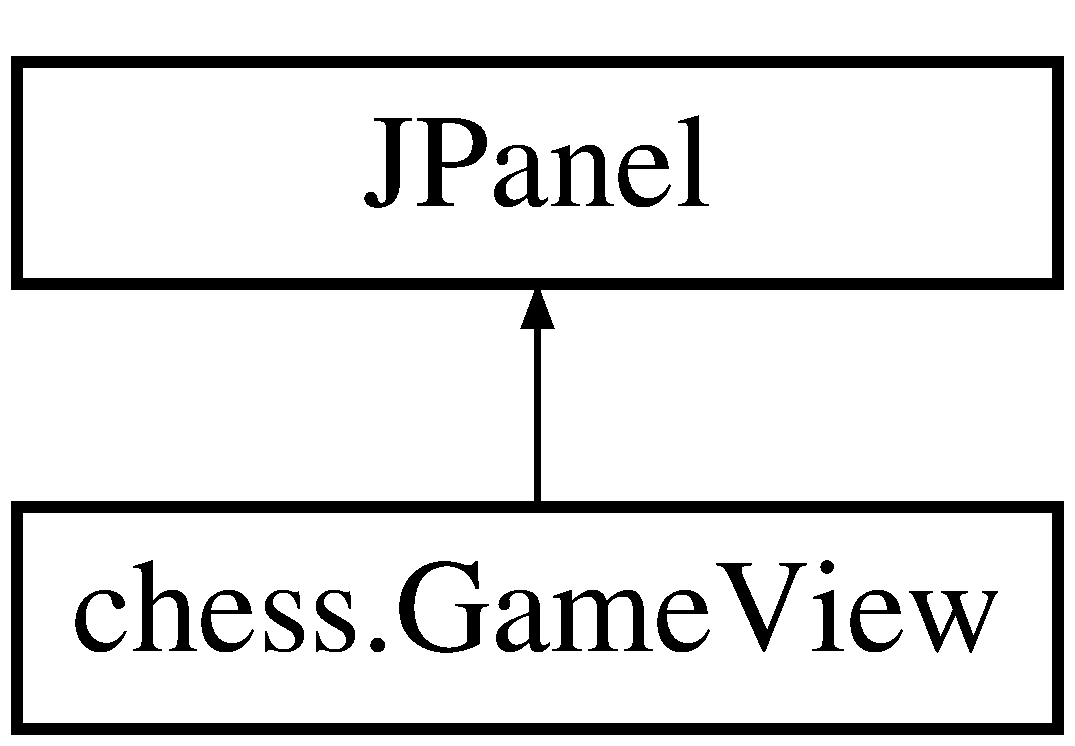
\includegraphics[height=2.000000cm]{classchess_1_1_game_view}
\end{center}
\end{figure}
\subsection*{Public Member Functions}
\begin{DoxyCompactItemize}
\item 
\hyperlink{classchess_1_1_game_view_a2164e6eddc14ec94819cf68f847cc9ec}{Game\+View} (\hyperlink{classchessboard_1_1_chess_board}{Chess\+Board} board, int tile\+\_\+size)
\item 
void \hyperlink{classchess_1_1_game_view_a8e8693a914d8545e48598460879592ec}{bind\+Game\+Controller} (\hyperlink{classchess_1_1_game_controller}{Game\+Controller} game\+\_\+controller)
\item 
void \hyperlink{classchess_1_1_game_view_afd6e597bb751b569b59db40ff455d694}{redraw} ()
\item 
void \hyperlink{classchess_1_1_game_view_abc5fa8b90f8041721614f2d56fec164e}{init\+Window} ()
\end{DoxyCompactItemize}
\subsection*{Protected Attributes}
\begin{DoxyCompactItemize}
\item 
\hypertarget{classchess_1_1_game_view_a0d299352c1008e693e6a27c6453e6bf3}{}\hyperlink{classchessboard_1_1_chess_board}{Chess\+Board} {\bfseries board}\label{classchess_1_1_game_view_a0d299352c1008e693e6a27c6453e6bf3}

\item 
\hypertarget{classchess_1_1_game_view_ac3ad8e3f6ed9f13a167b85c0ec90c934}{}\hyperlink{classchess_1_1_game_controller}{Game\+Controller} {\bfseries game\+\_\+controller}\label{classchess_1_1_game_view_ac3ad8e3f6ed9f13a167b85c0ec90c934}

\item 
\hypertarget{classchess_1_1_game_view_a05e36a24df714ada2e83a8dafa8deaa8}{}\hyperlink{classchess_1_1_chessboard___view}{Chessboard\+\_\+\+View} {\bfseries chessboard\+\_\+view}\label{classchess_1_1_game_view_a05e36a24df714ada2e83a8dafa8deaa8}

\item 
\hypertarget{classchess_1_1_game_view_a413033913e5b7dcefb33e93a5d3b0695}{}\hyperlink{classchess_1_1_menu_view}{Menu\+View} {\bfseries menu\+\_\+view}\label{classchess_1_1_game_view_a413033913e5b7dcefb33e93a5d3b0695}

\item 
\hypertarget{classchess_1_1_game_view_a4f9cd991b1b69aa71a6093063ae86744}{}int {\bfseries tile\+\_\+size}\label{classchess_1_1_game_view_a4f9cd991b1b69aa71a6093063ae86744}

\item 
\hypertarget{classchess_1_1_game_view_a1cfb8d5be090955b213d3ced4a8675dd}{}int {\bfseries view\+\_\+width}\label{classchess_1_1_game_view_a1cfb8d5be090955b213d3ced4a8675dd}

\item 
\hypertarget{classchess_1_1_game_view_a09be3aab3241803988d635105fd13332}{}int {\bfseries view\+\_\+height}\label{classchess_1_1_game_view_a09be3aab3241803988d635105fd13332}

\item 
\hypertarget{classchess_1_1_game_view_a80f5a13bb9998ac074fa370b7185437d}{}int {\bfseries board\+\_\+width}\label{classchess_1_1_game_view_a80f5a13bb9998ac074fa370b7185437d}

\item 
\hypertarget{classchess_1_1_game_view_ae955da73a217c4ebc61050c2c6263f80}{}int {\bfseries board\+\_\+height}\label{classchess_1_1_game_view_ae955da73a217c4ebc61050c2c6263f80}

\item 
\hypertarget{classchess_1_1_game_view_a30303cd2999aaee09917690d3f30b754}{}int {\bfseries menu\+\_\+width}\label{classchess_1_1_game_view_a30303cd2999aaee09917690d3f30b754}

\item 
\hypertarget{classchess_1_1_game_view_a095c5e95d97527bd2a0326252343f3c6}{}int {\bfseries menu\+\_\+height}\label{classchess_1_1_game_view_a095c5e95d97527bd2a0326252343f3c6}

\end{DoxyCompactItemize}


\subsection{Detailed Description}
Draw G\+U\+I for chess game \hyperlink{classchess_1_1_game}{Game} View consists of Chessboard View and Menu View 

\subsection{Constructor \& Destructor Documentation}
\hypertarget{classchess_1_1_game_view_a2164e6eddc14ec94819cf68f847cc9ec}{}\index{chess\+::\+Game\+View@{chess\+::\+Game\+View}!Game\+View@{Game\+View}}
\index{Game\+View@{Game\+View}!chess\+::\+Game\+View@{chess\+::\+Game\+View}}
\subsubsection[{Game\+View}]{\setlength{\rightskip}{0pt plus 5cm}chess.\+Game\+View.\+Game\+View (
\begin{DoxyParamCaption}
\item[{{\bf Chess\+Board}}]{board, }
\item[{int}]{tile\+\_\+size}
\end{DoxyParamCaption}
)\hspace{0.3cm}{\ttfamily [inline]}}\label{classchess_1_1_game_view_a2164e6eddc14ec94819cf68f847cc9ec}
Constructor\+: init game view 
\begin{DoxyParams}{Parameters}
{\em board} & the chessboard that we are using now \\
\hline
{\em tile\+\_\+size} & this size of tile \\
\hline
\end{DoxyParams}


\subsection{Member Function Documentation}
\hypertarget{classchess_1_1_game_view_a8e8693a914d8545e48598460879592ec}{}\index{chess\+::\+Game\+View@{chess\+::\+Game\+View}!bind\+Game\+Controller@{bind\+Game\+Controller}}
\index{bind\+Game\+Controller@{bind\+Game\+Controller}!chess\+::\+Game\+View@{chess\+::\+Game\+View}}
\subsubsection[{bind\+Game\+Controller}]{\setlength{\rightskip}{0pt plus 5cm}void chess.\+Game\+View.\+bind\+Game\+Controller (
\begin{DoxyParamCaption}
\item[{{\bf Game\+Controller}}]{game\+\_\+controller}
\end{DoxyParamCaption}
)\hspace{0.3cm}{\ttfamily [inline]}}\label{classchess_1_1_game_view_a8e8693a914d8545e48598460879592ec}
Bing game controller to this game view 
\begin{DoxyParams}{Parameters}
{\em game\+\_\+controller} & the game controller that we are going to use. \\
\hline
\end{DoxyParams}
\hypertarget{classchess_1_1_game_view_abc5fa8b90f8041721614f2d56fec164e}{}\index{chess\+::\+Game\+View@{chess\+::\+Game\+View}!init\+Window@{init\+Window}}
\index{init\+Window@{init\+Window}!chess\+::\+Game\+View@{chess\+::\+Game\+View}}
\subsubsection[{init\+Window}]{\setlength{\rightskip}{0pt plus 5cm}void chess.\+Game\+View.\+init\+Window (
\begin{DoxyParamCaption}
{}
\end{DoxyParamCaption}
)\hspace{0.3cm}{\ttfamily [inline]}}\label{classchess_1_1_game_view_abc5fa8b90f8041721614f2d56fec164e}
Initialize game window \hypertarget{classchess_1_1_game_view_afd6e597bb751b569b59db40ff455d694}{}\index{chess\+::\+Game\+View@{chess\+::\+Game\+View}!redraw@{redraw}}
\index{redraw@{redraw}!chess\+::\+Game\+View@{chess\+::\+Game\+View}}
\subsubsection[{redraw}]{\setlength{\rightskip}{0pt plus 5cm}void chess.\+Game\+View.\+redraw (
\begin{DoxyParamCaption}
{}
\end{DoxyParamCaption}
)\hspace{0.3cm}{\ttfamily [inline]}}\label{classchess_1_1_game_view_afd6e597bb751b569b59db40ff455d694}
redraw the whole game view 

The documentation for this class was generated from the following file\+:\begin{DoxyCompactItemize}
\item 
src/chess/Game\+View.\+java\end{DoxyCompactItemize}

\hypertarget{classpiece_1_1_king}{}\section{piece.\+King Class Reference}
\label{classpiece_1_1_king}\index{piece.\+King@{piece.\+King}}
Inheritance diagram for piece.\+King\+:\begin{figure}[H]
\begin{center}
\leavevmode
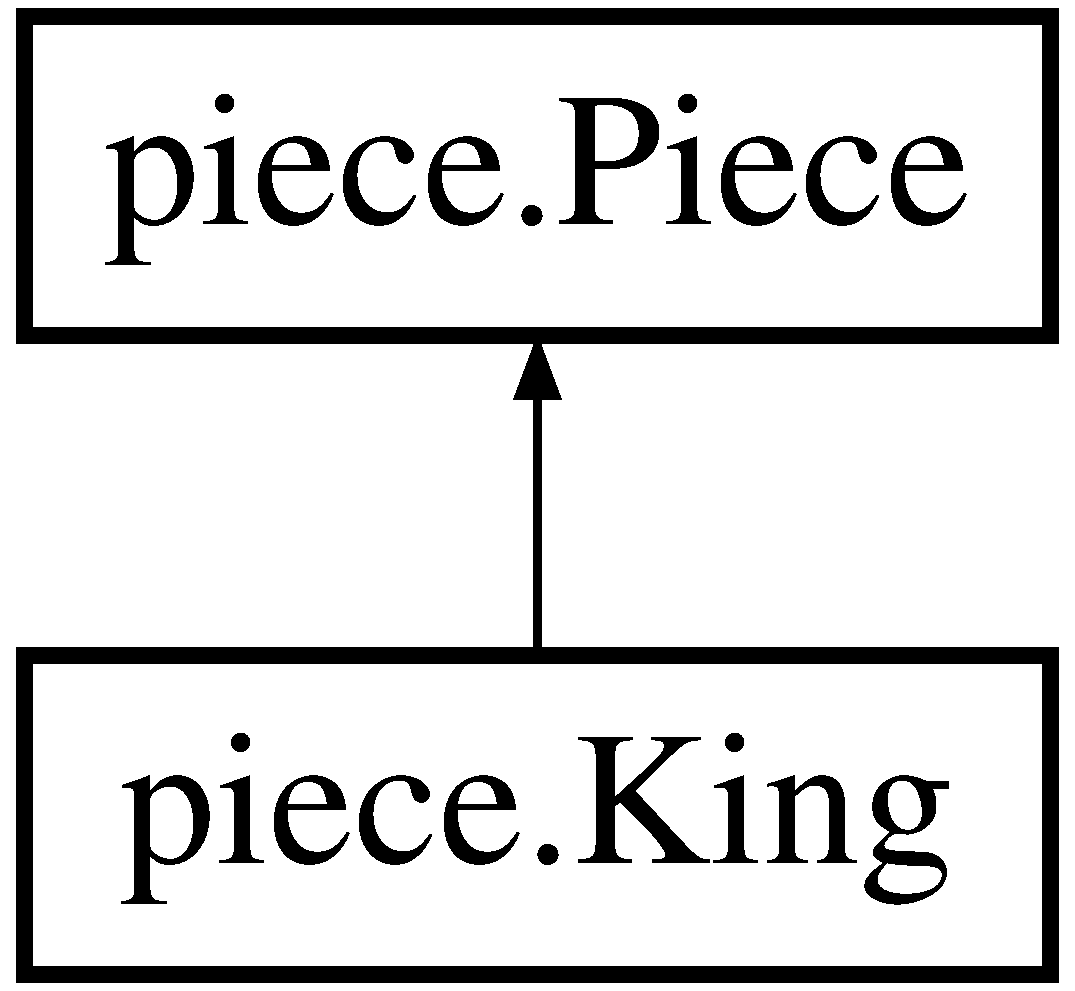
\includegraphics[height=2.000000cm]{classpiece_1_1_king}
\end{center}
\end{figure}
\subsection*{Public Member Functions}
\begin{DoxyCompactItemize}
\item 
\hyperlink{classpiece_1_1_king_a8d0f35dc55155899732ded91c9e515a1}{King} (\hyperlink{classchessboard_1_1_chess_board}{Chess\+Board} board, \hyperlink{enumchessboard_1_1_player}{Player} player)
\item 
Array\+List$<$ \hyperlink{classpiece_1_1_coordinate}{Coordinate} $>$ \hyperlink{classpiece_1_1_king_a4b21f711fd2e4ac41b4bef0855652e95}{get\+Possible\+Move\+Coordinate} ()
\item 
boolean \hyperlink{classpiece_1_1_king_a1f07ebf057c6ae0c607c83b58f2e12c6}{is\+In\+Check} ()
\end{DoxyCompactItemize}
\subsection*{Additional Inherited Members}


\subsection{Detailed Description}
Created by wangyiyi on 2/12/15. 

\subsection{Constructor \& Destructor Documentation}
\hypertarget{classpiece_1_1_king_a8d0f35dc55155899732ded91c9e515a1}{}\index{piece\+::\+King@{piece\+::\+King}!King@{King}}
\index{King@{King}!piece\+::\+King@{piece\+::\+King}}
\subsubsection[{King}]{\setlength{\rightskip}{0pt plus 5cm}piece.\+King.\+King (
\begin{DoxyParamCaption}
\item[{{\bf Chess\+Board}}]{board, }
\item[{{\bf Player}}]{player}
\end{DoxyParamCaption}
)\hspace{0.3cm}{\ttfamily [inline]}}\label{classpiece_1_1_king_a8d0f35dc55155899732ded91c9e515a1}
Constructor\+: Initialize a \hyperlink{classpiece_1_1_king}{King} Object 
\begin{DoxyParams}{Parameters}
{\em board} & the board we are currently using \\
\hline
{\em player} & the player that holds the piece \\
\hline
\end{DoxyParams}


\subsection{Member Function Documentation}
\hypertarget{classpiece_1_1_king_a4b21f711fd2e4ac41b4bef0855652e95}{}\index{piece\+::\+King@{piece\+::\+King}!get\+Possible\+Move\+Coordinate@{get\+Possible\+Move\+Coordinate}}
\index{get\+Possible\+Move\+Coordinate@{get\+Possible\+Move\+Coordinate}!piece\+::\+King@{piece\+::\+King}}
\subsubsection[{get\+Possible\+Move\+Coordinate}]{\setlength{\rightskip}{0pt plus 5cm}Array\+List$<${\bf Coordinate}$>$ piece.\+King.\+get\+Possible\+Move\+Coordinate (
\begin{DoxyParamCaption}
{}
\end{DoxyParamCaption}
)\hspace{0.3cm}{\ttfamily [inline]}}\label{classpiece_1_1_king_a4b21f711fd2e4ac41b4bef0855652e95}
Get all possible move coordinates for this king piece at current coordinate \begin{DoxyVerb}              P: this piece
              @: Possible coordinates to move
@ @ @
@ P @
@ @ @
\end{DoxyVerb}


\begin{DoxyReturn}{Returns}
Array\+List$<$\+Coordinate$>$ Object that contains all possible move coordinates. 
\end{DoxyReturn}
\hypertarget{classpiece_1_1_king_a1f07ebf057c6ae0c607c83b58f2e12c6}{}\index{piece\+::\+King@{piece\+::\+King}!is\+In\+Check@{is\+In\+Check}}
\index{is\+In\+Check@{is\+In\+Check}!piece\+::\+King@{piece\+::\+King}}
\subsubsection[{is\+In\+Check}]{\setlength{\rightskip}{0pt plus 5cm}boolean piece.\+King.\+is\+In\+Check (
\begin{DoxyParamCaption}
{}
\end{DoxyParamCaption}
)\hspace{0.3cm}{\ttfamily [inline]}}\label{classpiece_1_1_king_a1f07ebf057c6ae0c607c83b58f2e12c6}
Check whether the king is in check \begin{DoxyReturn}{Returns}
true if the king is in check; otherwise return false 
\end{DoxyReturn}


The documentation for this class was generated from the following file\+:\begin{DoxyCompactItemize}
\item 
src/piece/King.\+java\end{DoxyCompactItemize}

\hypertarget{classunit__test_1_1_king_test}{}\section{unit\+\_\+test.\+King\+Test Class Reference}
\label{classunit__test_1_1_king_test}\index{unit\+\_\+test.\+King\+Test@{unit\+\_\+test.\+King\+Test}}
\subsection*{Public Member Functions}
\begin{DoxyCompactItemize}
\item 
void \hyperlink{classunit__test_1_1_king_test_ab1dacd878b628f0a4235bf8c2c07a3e2}{test\+Get\+Possible\+Move\+Coordinate} ()  throws Exception 
\item 
\hypertarget{classunit__test_1_1_king_test_a5869c0c6be7a8bcdac6d15b2115e965f}{}void {\bfseries test\+Is\+In\+Check} ()  throws Exception \label{classunit__test_1_1_king_test_a5869c0c6be7a8bcdac6d15b2115e965f}

\end{DoxyCompactItemize}


\subsection{Member Function Documentation}
\hypertarget{classunit__test_1_1_king_test_ab1dacd878b628f0a4235bf8c2c07a3e2}{}\index{unit\+\_\+test\+::\+King\+Test@{unit\+\_\+test\+::\+King\+Test}!test\+Get\+Possible\+Move\+Coordinate@{test\+Get\+Possible\+Move\+Coordinate}}
\index{test\+Get\+Possible\+Move\+Coordinate@{test\+Get\+Possible\+Move\+Coordinate}!unit\+\_\+test\+::\+King\+Test@{unit\+\_\+test\+::\+King\+Test}}
\subsubsection[{test\+Get\+Possible\+Move\+Coordinate}]{\setlength{\rightskip}{0pt plus 5cm}void unit\+\_\+test.\+King\+Test.\+test\+Get\+Possible\+Move\+Coordinate (
\begin{DoxyParamCaption}
{}
\end{DoxyParamCaption}
) throws Exception\hspace{0.3cm}{\ttfamily [inline]}}\label{classunit__test_1_1_king_test_ab1dacd878b628f0a4235bf8c2c07a3e2}
test valid possible moves 
\begin{DoxyExceptions}{Exceptions}
{\em Exception} & \\
\hline
\end{DoxyExceptions}


The documentation for this class was generated from the following file\+:\begin{DoxyCompactItemize}
\item 
unit\+\_\+test/King\+Test.\+java\end{DoxyCompactItemize}

\hypertarget{classpiece_1_1_knight}{}\section{piece.\+Knight Class Reference}
\label{classpiece_1_1_knight}\index{piece.\+Knight@{piece.\+Knight}}
Inheritance diagram for piece.\+Knight\+:\begin{figure}[H]
\begin{center}
\leavevmode
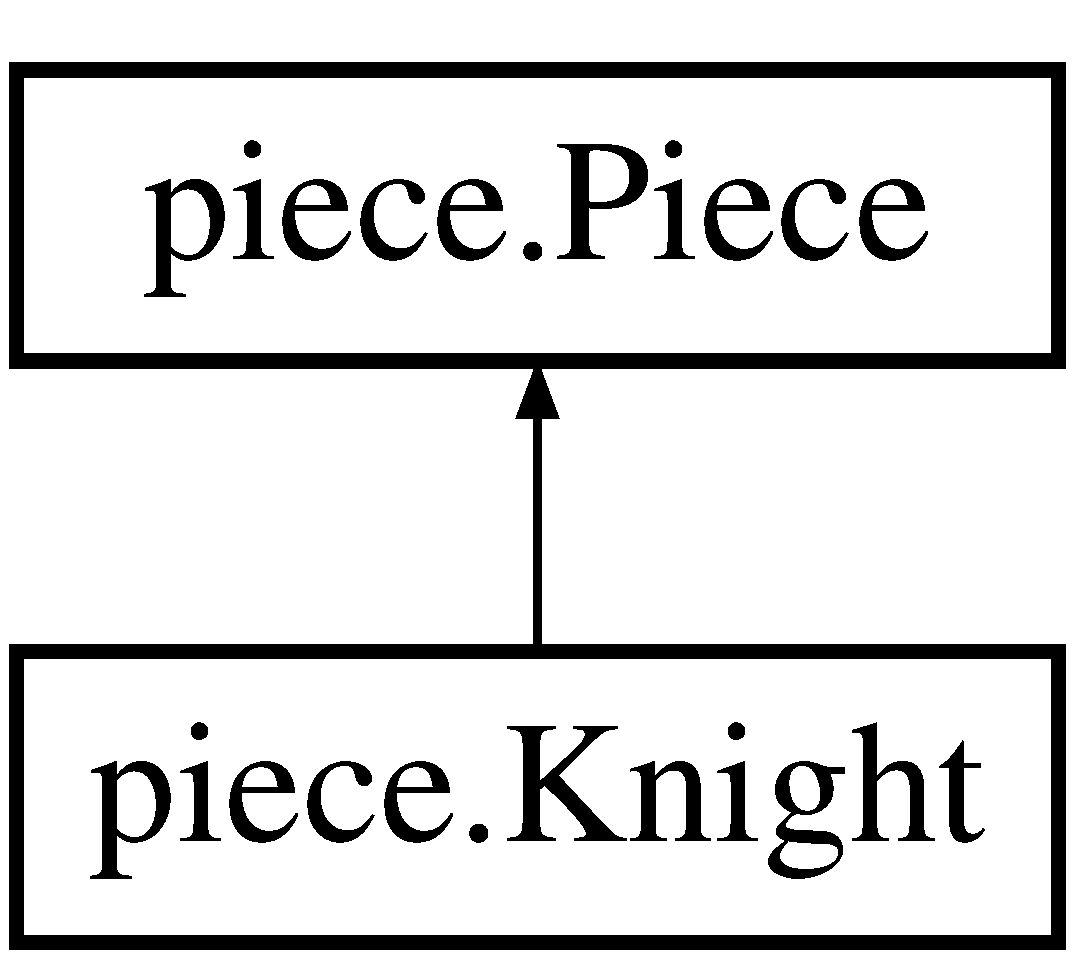
\includegraphics[height=2.000000cm]{classpiece_1_1_knight}
\end{center}
\end{figure}
\subsection*{Public Member Functions}
\begin{DoxyCompactItemize}
\item 
\hyperlink{classpiece_1_1_knight_a74e148bd203ec7885971091cff1208ab}{Knight} (\hyperlink{classchessboard_1_1_chess_board}{Chess\+Board} board, \hyperlink{enumchessboard_1_1_player}{Player} player)
\item 
Array\+List$<$ \hyperlink{classpiece_1_1_coordinate}{Coordinate} $>$ \hyperlink{classpiece_1_1_knight_a1ac2e811908e6261d7e90bb5bed071c6}{get\+Possible\+Move\+Coordinate} ()
\end{DoxyCompactItemize}
\subsection*{Additional Inherited Members}


\subsection{Detailed Description}
Created by wangyiyi on 2/12/15. 

\subsection{Constructor \& Destructor Documentation}
\hypertarget{classpiece_1_1_knight_a74e148bd203ec7885971091cff1208ab}{}\index{piece\+::\+Knight@{piece\+::\+Knight}!Knight@{Knight}}
\index{Knight@{Knight}!piece\+::\+Knight@{piece\+::\+Knight}}
\subsubsection[{Knight}]{\setlength{\rightskip}{0pt plus 5cm}piece.\+Knight.\+Knight (
\begin{DoxyParamCaption}
\item[{{\bf Chess\+Board}}]{board, }
\item[{{\bf Player}}]{player}
\end{DoxyParamCaption}
)\hspace{0.3cm}{\ttfamily [inline]}}\label{classpiece_1_1_knight_a74e148bd203ec7885971091cff1208ab}
Constructor\+: initialize a \hyperlink{classpiece_1_1_knight}{Knight} Object 
\begin{DoxyParams}{Parameters}
{\em board} & the board that we are currently using \\
\hline
{\em player} & the player that holds the piece \\
\hline
\end{DoxyParams}


\subsection{Member Function Documentation}
\hypertarget{classpiece_1_1_knight_a1ac2e811908e6261d7e90bb5bed071c6}{}\index{piece\+::\+Knight@{piece\+::\+Knight}!get\+Possible\+Move\+Coordinate@{get\+Possible\+Move\+Coordinate}}
\index{get\+Possible\+Move\+Coordinate@{get\+Possible\+Move\+Coordinate}!piece\+::\+Knight@{piece\+::\+Knight}}
\subsubsection[{get\+Possible\+Move\+Coordinate}]{\setlength{\rightskip}{0pt plus 5cm}Array\+List$<${\bf Coordinate}$>$ piece.\+Knight.\+get\+Possible\+Move\+Coordinate (
\begin{DoxyParamCaption}
{}
\end{DoxyParamCaption}
)\hspace{0.3cm}{\ttfamily [inline]}}\label{classpiece_1_1_knight_a1ac2e811908e6261d7e90bb5bed071c6}
Get all possible move coordinates for this knight piece at current coordinate

\begin{DoxyVerb}          @      @
   @                   @       P: this piece
            P                 @: Possible coordinates to move
   @                   @
         @       @
\end{DoxyVerb}


\begin{DoxyReturn}{Returns}
Array\+List$<$\+Coordinate$>$ Object that contains all possible move coordinates. 
\end{DoxyReturn}


The documentation for this class was generated from the following file\+:\begin{DoxyCompactItemize}
\item 
src/piece/Knight.\+java\end{DoxyCompactItemize}

\hypertarget{classunit__test_1_1_knight_test}{}\section{unit\+\_\+test.\+Knight\+Test Class Reference}
\label{classunit__test_1_1_knight_test}\index{unit\+\_\+test.\+Knight\+Test@{unit\+\_\+test.\+Knight\+Test}}
\subsection*{Public Member Functions}
\begin{DoxyCompactItemize}
\item 
void \hyperlink{classunit__test_1_1_knight_test_a5c0efc621ef5bb4e82f5be72de53e30d}{test\+Get\+Possible\+Move\+Coordinate} ()  throws Exception 
\end{DoxyCompactItemize}


\subsection{Member Function Documentation}
\hypertarget{classunit__test_1_1_knight_test_a5c0efc621ef5bb4e82f5be72de53e30d}{}\index{unit\+\_\+test\+::\+Knight\+Test@{unit\+\_\+test\+::\+Knight\+Test}!test\+Get\+Possible\+Move\+Coordinate@{test\+Get\+Possible\+Move\+Coordinate}}
\index{test\+Get\+Possible\+Move\+Coordinate@{test\+Get\+Possible\+Move\+Coordinate}!unit\+\_\+test\+::\+Knight\+Test@{unit\+\_\+test\+::\+Knight\+Test}}
\subsubsection[{test\+Get\+Possible\+Move\+Coordinate}]{\setlength{\rightskip}{0pt plus 5cm}void unit\+\_\+test.\+Knight\+Test.\+test\+Get\+Possible\+Move\+Coordinate (
\begin{DoxyParamCaption}
{}
\end{DoxyParamCaption}
) throws Exception\hspace{0.3cm}{\ttfamily [inline]}}\label{classunit__test_1_1_knight_test_a5c0efc621ef5bb4e82f5be72de53e30d}
test valid possible moves 

The documentation for this class was generated from the following file\+:\begin{DoxyCompactItemize}
\item 
unit\+\_\+test/Knight\+Test.\+java\end{DoxyCompactItemize}

\hypertarget{classpiece_1_1_lancer}{}\section{piece.\+Lancer Class Reference}
\label{classpiece_1_1_lancer}\index{piece.\+Lancer@{piece.\+Lancer}}
Inheritance diagram for piece.\+Lancer\+:\begin{figure}[H]
\begin{center}
\leavevmode
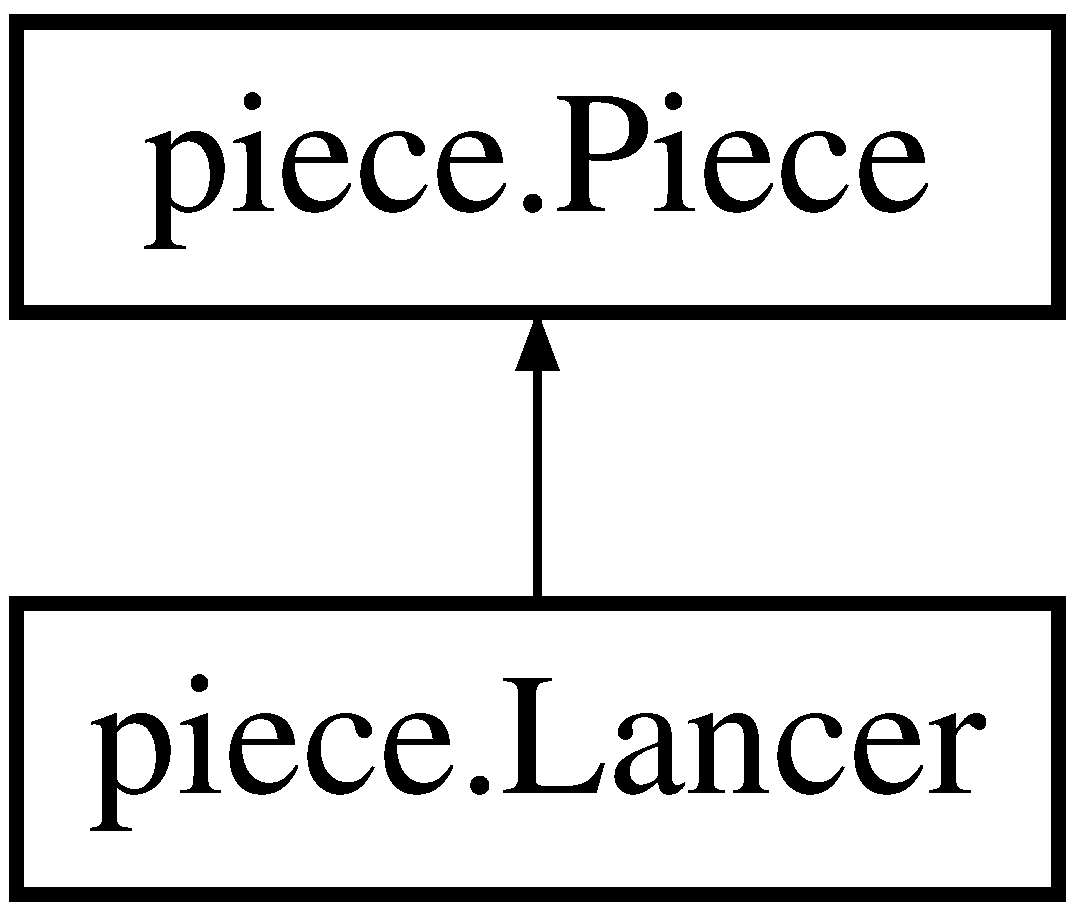
\includegraphics[height=2.000000cm]{classpiece_1_1_lancer}
\end{center}
\end{figure}
\subsection*{Public Member Functions}
\begin{DoxyCompactItemize}
\item 
\hyperlink{classpiece_1_1_lancer_a50616ad4693ed4d3923a447ecc36d893}{Lancer} (\hyperlink{classchessboard_1_1_chess_board}{Chess\+Board} board, \hyperlink{enumchessboard_1_1_player}{Player} player)
\item 
Array\+List$<$ \hyperlink{classpiece_1_1_coordinate}{Coordinate} $>$ \hyperlink{classpiece_1_1_lancer_ad347a5eb8ae6db14e7a112ae640d3c88}{get\+Possible\+Move\+Coordinate} ()
\end{DoxyCompactItemize}
\subsection*{Additional Inherited Members}


\subsection{Detailed Description}
Created by wangyiyi on 2/18/15. 

\subsection{Constructor \& Destructor Documentation}
\hypertarget{classpiece_1_1_lancer_a50616ad4693ed4d3923a447ecc36d893}{}\index{piece\+::\+Lancer@{piece\+::\+Lancer}!Lancer@{Lancer}}
\index{Lancer@{Lancer}!piece\+::\+Lancer@{piece\+::\+Lancer}}
\subsubsection[{Lancer}]{\setlength{\rightskip}{0pt plus 5cm}piece.\+Lancer.\+Lancer (
\begin{DoxyParamCaption}
\item[{{\bf Chess\+Board}}]{board, }
\item[{{\bf Player}}]{player}
\end{DoxyParamCaption}
)\hspace{0.3cm}{\ttfamily [inline]}}\label{classpiece_1_1_lancer_a50616ad4693ed4d3923a447ecc36d893}
Constructor\+: initialize an \hyperlink{classpiece_1_1_lancer}{Lancer} Object 
\begin{DoxyParams}{Parameters}
{\em board} & the board that we are currently using \\
\hline
{\em player} & the player that holds the piece \\
\hline
\end{DoxyParams}


\subsection{Member Function Documentation}
\hypertarget{classpiece_1_1_lancer_ad347a5eb8ae6db14e7a112ae640d3c88}{}\index{piece\+::\+Lancer@{piece\+::\+Lancer}!get\+Possible\+Move\+Coordinate@{get\+Possible\+Move\+Coordinate}}
\index{get\+Possible\+Move\+Coordinate@{get\+Possible\+Move\+Coordinate}!piece\+::\+Lancer@{piece\+::\+Lancer}}
\subsubsection[{get\+Possible\+Move\+Coordinate}]{\setlength{\rightskip}{0pt plus 5cm}Array\+List$<${\bf Coordinate}$>$ piece.\+Lancer.\+get\+Possible\+Move\+Coordinate (
\begin{DoxyParamCaption}
{}
\end{DoxyParamCaption}
)\hspace{0.3cm}{\ttfamily [inline]}}\label{classpiece_1_1_lancer_ad347a5eb8ae6db14e7a112ae640d3c88}
Attack and Move coordinate\+: \begin{DoxyVerb}      #
    # # #                  #: possible moves
  # # p # #                P: lancer
\end{DoxyVerb}


if there is enemy/friend on left/top/right that block the way, then archer cannot go further

\begin{DoxyReturn}{Returns}
Array\+List$<$\+Coordinate$>$ Object that contains all possible move coordinates. 
\end{DoxyReturn}


The documentation for this class was generated from the following file\+:\begin{DoxyCompactItemize}
\item 
src/piece/Lancer.\+java\end{DoxyCompactItemize}

\hypertarget{classunit__test_1_1_lancer_test}{}\section{unit\+\_\+test.\+Lancer\+Test Class Reference}
\label{classunit__test_1_1_lancer_test}\index{unit\+\_\+test.\+Lancer\+Test@{unit\+\_\+test.\+Lancer\+Test}}
Inheritance diagram for unit\+\_\+test.\+Lancer\+Test\+:\begin{figure}[H]
\begin{center}
\leavevmode
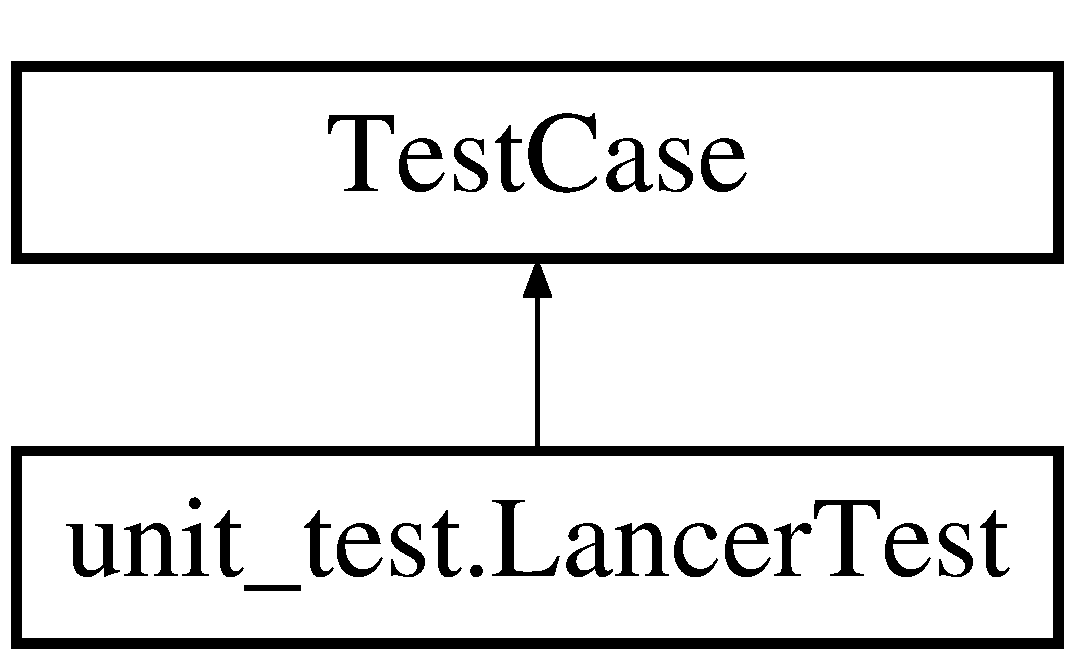
\includegraphics[height=2.000000cm]{classunit__test_1_1_lancer_test}
\end{center}
\end{figure}
\subsection*{Public Member Functions}
\begin{DoxyCompactItemize}
\item 
void \hyperlink{classunit__test_1_1_lancer_test_a81470104b4b538ecc32c8343f400385c}{test\+Get\+Possible\+Move\+Coordinate} ()  throws Exception 
\end{DoxyCompactItemize}


\subsection{Member Function Documentation}
\hypertarget{classunit__test_1_1_lancer_test_a81470104b4b538ecc32c8343f400385c}{}\index{unit\+\_\+test\+::\+Lancer\+Test@{unit\+\_\+test\+::\+Lancer\+Test}!test\+Get\+Possible\+Move\+Coordinate@{test\+Get\+Possible\+Move\+Coordinate}}
\index{test\+Get\+Possible\+Move\+Coordinate@{test\+Get\+Possible\+Move\+Coordinate}!unit\+\_\+test\+::\+Lancer\+Test@{unit\+\_\+test\+::\+Lancer\+Test}}
\subsubsection[{test\+Get\+Possible\+Move\+Coordinate}]{\setlength{\rightskip}{0pt plus 5cm}void unit\+\_\+test.\+Lancer\+Test.\+test\+Get\+Possible\+Move\+Coordinate (
\begin{DoxyParamCaption}
{}
\end{DoxyParamCaption}
) throws Exception\hspace{0.3cm}{\ttfamily [inline]}}\label{classunit__test_1_1_lancer_test_a81470104b4b538ecc32c8343f400385c}
test valid possible moves 

The documentation for this class was generated from the following file\+:\begin{DoxyCompactItemize}
\item 
src/unit\+\_\+test/Lancer\+Test.\+java\end{DoxyCompactItemize}

\hypertarget{classchess_1_1_menu_view}{}\section{chess.\+Menu\+View Class Reference}
\label{classchess_1_1_menu_view}\index{chess.\+Menu\+View@{chess.\+Menu\+View}}
Inheritance diagram for chess.\+Menu\+View\+:\begin{figure}[H]
\begin{center}
\leavevmode
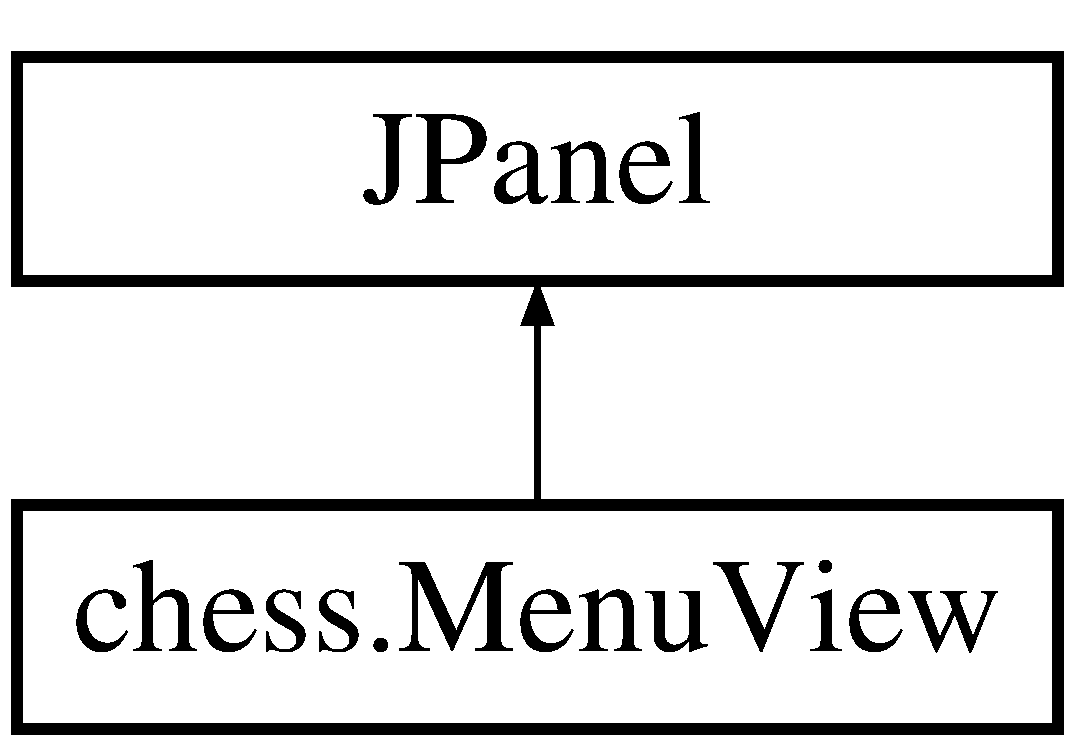
\includegraphics[height=2.000000cm]{classchess_1_1_menu_view}
\end{center}
\end{figure}
\subsection*{Public Member Functions}
\begin{DoxyCompactItemize}
\item 
\hyperlink{classchess_1_1_menu_view_a32fab9a8ed947bdf0552c22c781fe223}{Menu\+View} (int width, int height, final \hyperlink{classchess_1_1_game_view}{Game\+View} game\+\_\+view)
\item 
void \hyperlink{classchess_1_1_menu_view_ab6387368d456b68343d2703db50dfcad}{paint} (Graphics g)
\item 
void \hyperlink{classchess_1_1_menu_view_afa544160eff3554f30c96c24ef5c7e0f}{draw\+Menu} (int player1\+\_\+score, int player2\+\_\+score, String message)
\end{DoxyCompactItemize}
\subsection*{Protected Attributes}
\begin{DoxyCompactItemize}
\item 
\hypertarget{classchess_1_1_menu_view_adefa172949408b1790ff096f9b54a608}{}\hyperlink{classchess_1_1_game_view}{Game\+View} {\bfseries game\+\_\+view}\label{classchess_1_1_menu_view_adefa172949408b1790ff096f9b54a608}

\item 
\hypertarget{classchess_1_1_menu_view_a05538a9fb9546d229bcad6b8a08c9415}{}J\+Button {\bfseries start\+\_\+btn}\label{classchess_1_1_menu_view_a05538a9fb9546d229bcad6b8a08c9415}

\item 
\hypertarget{classchess_1_1_menu_view_a65045bb89a83e5c5e9631f8e158c3a40}{}J\+Button {\bfseries restart\+\_\+btn}\label{classchess_1_1_menu_view_a65045bb89a83e5c5e9631f8e158c3a40}

\item 
\hypertarget{classchess_1_1_menu_view_aa6c03d8d38402aa02ca348bbba9e2980}{}J\+Button {\bfseries forfeit\+\_\+btn}\label{classchess_1_1_menu_view_aa6c03d8d38402aa02ca348bbba9e2980}

\item 
\hypertarget{classchess_1_1_menu_view_a14d65117b41c76711579633c76014de3}{}J\+Button {\bfseries undo\+\_\+btn}\label{classchess_1_1_menu_view_a14d65117b41c76711579633c76014de3}

\item 
\hypertarget{classchess_1_1_menu_view_a9d6092188ac2d5bb418a7f8fdc7b8ac5}{}J\+Button {\bfseries player1\+\_\+btn}\label{classchess_1_1_menu_view_a9d6092188ac2d5bb418a7f8fdc7b8ac5}

\item 
\hypertarget{classchess_1_1_menu_view_a59fe7d3feb2f71eade47ee40d42179f2}{}J\+Button {\bfseries player2\+\_\+btn}\label{classchess_1_1_menu_view_a59fe7d3feb2f71eade47ee40d42179f2}

\end{DoxyCompactItemize}


\subsection{Detailed Description}
This class is used to draw menu 

\subsection{Constructor \& Destructor Documentation}
\hypertarget{classchess_1_1_menu_view_a32fab9a8ed947bdf0552c22c781fe223}{}\index{chess\+::\+Menu\+View@{chess\+::\+Menu\+View}!Menu\+View@{Menu\+View}}
\index{Menu\+View@{Menu\+View}!chess\+::\+Menu\+View@{chess\+::\+Menu\+View}}
\subsubsection[{Menu\+View}]{\setlength{\rightskip}{0pt plus 5cm}chess.\+Menu\+View.\+Menu\+View (
\begin{DoxyParamCaption}
\item[{int}]{width, }
\item[{int}]{height, }
\item[{final {\bf Game\+View}}]{game\+\_\+view}
\end{DoxyParamCaption}
)\hspace{0.3cm}{\ttfamily [inline]}}\label{classchess_1_1_menu_view_a32fab9a8ed947bdf0552c22c781fe223}
\hyperlink{classchess_1_1_menu_view}{Menu\+View} constructor This constructor is used to put several components on panel eg\+: start button, restart button, forfeit button, undo button, etc. 
\begin{DoxyParams}{Parameters}
{\em width} & \\
\hline
{\em height} & \\
\hline
\end{DoxyParams}
Clicked start button 
\begin{DoxyParams}{Parameters}
{\em e} & \\
\hline
\end{DoxyParams}
Clicked restart button 
\begin{DoxyParams}{Parameters}
{\em e} & \\
\hline
\end{DoxyParams}
Clicked forfeit button 
\begin{DoxyParams}{Parameters}
{\em e} & \\
\hline
\end{DoxyParams}
Clicked undo button 
\begin{DoxyParams}{Parameters}
{\em e} & \\
\hline
{\em e} & \\
\hline
{\em e} & \\
\hline
\end{DoxyParams}


\subsection{Member Function Documentation}
\hypertarget{classchess_1_1_menu_view_afa544160eff3554f30c96c24ef5c7e0f}{}\index{chess\+::\+Menu\+View@{chess\+::\+Menu\+View}!draw\+Menu@{draw\+Menu}}
\index{draw\+Menu@{draw\+Menu}!chess\+::\+Menu\+View@{chess\+::\+Menu\+View}}
\subsubsection[{draw\+Menu}]{\setlength{\rightskip}{0pt plus 5cm}void chess.\+Menu\+View.\+draw\+Menu (
\begin{DoxyParamCaption}
\item[{int}]{player1\+\_\+score, }
\item[{int}]{player2\+\_\+score, }
\item[{String}]{message}
\end{DoxyParamCaption}
)\hspace{0.3cm}{\ttfamily [inline]}}\label{classchess_1_1_menu_view_afa544160eff3554f30c96c24ef5c7e0f}
update player1\+\_\+score, player2\+\_\+score, message. repaint the menu canvas.


\begin{DoxyParams}{Parameters}
{\em player1\+\_\+score} & new player1 score \\
\hline
{\em player2\+\_\+score} & new player2 score \\
\hline
{\em message} & new message \\
\hline
\end{DoxyParams}
\hypertarget{classchess_1_1_menu_view_ab6387368d456b68343d2703db50dfcad}{}\index{chess\+::\+Menu\+View@{chess\+::\+Menu\+View}!paint@{paint}}
\index{paint@{paint}!chess\+::\+Menu\+View@{chess\+::\+Menu\+View}}
\subsubsection[{paint}]{\setlength{\rightskip}{0pt plus 5cm}void chess.\+Menu\+View.\+paint (
\begin{DoxyParamCaption}
\item[{Graphics}]{g}
\end{DoxyParamCaption}
)\hspace{0.3cm}{\ttfamily [inline]}}\label{classchess_1_1_menu_view_ab6387368d456b68343d2703db50dfcad}
Draw menu 
\begin{DoxyParams}{Parameters}
{\em g} & \\
\hline
\end{DoxyParams}


The documentation for this class was generated from the following file\+:\begin{DoxyCompactItemize}
\item 
src/chess/Menu\+View.\+java\end{DoxyCompactItemize}

\hypertarget{classpiece_1_1_pawn}{}\section{piece.\+Pawn Class Reference}
\label{classpiece_1_1_pawn}\index{piece.\+Pawn@{piece.\+Pawn}}
Inheritance diagram for piece.\+Pawn\+:\begin{figure}[H]
\begin{center}
\leavevmode
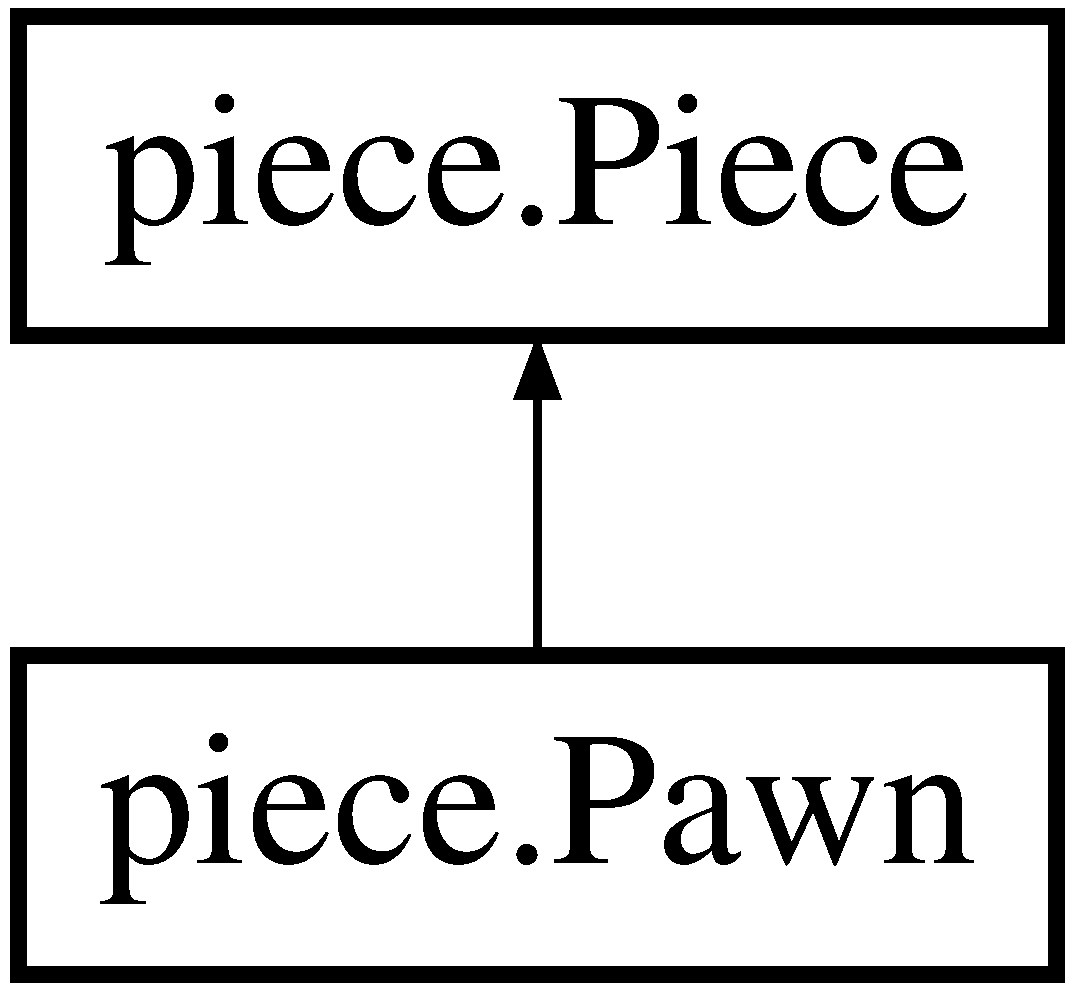
\includegraphics[height=2.000000cm]{classpiece_1_1_pawn}
\end{center}
\end{figure}
\subsection*{Public Member Functions}
\begin{DoxyCompactItemize}
\item 
\hyperlink{classpiece_1_1_pawn_a4f7b4f8e849019f15398ed007e89e942}{Pawn} (\hyperlink{classchess_1_1_chess_board}{Chess\+Board} board, \hyperlink{enumchess_1_1_player}{Player} player)
\item 
Array\+List$<$ \hyperlink{classpiece_1_1_coordinate}{Coordinate} $>$ \hyperlink{classpiece_1_1_pawn_aca9da51119ce8972a9897a69c3ef5033}{get\+Possible\+Move\+Coordinate} ()
\item 
boolean \hyperlink{classpiece_1_1_pawn_adaf68cbd144297f69817229018d54e36}{set\+Coordinate} (int x, int y)
\item 
boolean \hyperlink{classpiece_1_1_pawn_a266eebe5a89125e60a4eb9bb345bd16e}{set\+Coordinate\+Without\+Changing\+First\+Time\+Move\+Flag} (int x, int y)
\end{DoxyCompactItemize}
\subsection*{Additional Inherited Members}


\subsection{Detailed Description}
Created by wangyiyi on 2/12/15. 

\subsection{Constructor \& Destructor Documentation}
\hypertarget{classpiece_1_1_pawn_a4f7b4f8e849019f15398ed007e89e942}{}\index{piece\+::\+Pawn@{piece\+::\+Pawn}!Pawn@{Pawn}}
\index{Pawn@{Pawn}!piece\+::\+Pawn@{piece\+::\+Pawn}}
\subsubsection[{Pawn}]{\setlength{\rightskip}{0pt plus 5cm}piece.\+Pawn.\+Pawn (
\begin{DoxyParamCaption}
\item[{{\bf Chess\+Board}}]{board, }
\item[{{\bf Player}}]{player}
\end{DoxyParamCaption}
)\hspace{0.3cm}{\ttfamily [inline]}}\label{classpiece_1_1_pawn_a4f7b4f8e849019f15398ed007e89e942}
Constructor\+: initialize a \hyperlink{classpiece_1_1_pawn}{Pawn} Object 
\begin{DoxyParams}{Parameters}
{\em board} & the board that we are currently using \\
\hline
{\em player} & the player that holds the piece \\
\hline
\end{DoxyParams}


\subsection{Member Function Documentation}
\hypertarget{classpiece_1_1_pawn_aca9da51119ce8972a9897a69c3ef5033}{}\index{piece\+::\+Pawn@{piece\+::\+Pawn}!get\+Possible\+Move\+Coordinate@{get\+Possible\+Move\+Coordinate}}
\index{get\+Possible\+Move\+Coordinate@{get\+Possible\+Move\+Coordinate}!piece\+::\+Pawn@{piece\+::\+Pawn}}
\subsubsection[{get\+Possible\+Move\+Coordinate}]{\setlength{\rightskip}{0pt plus 5cm}Array\+List$<${\bf Coordinate}$>$ piece.\+Pawn.\+get\+Possible\+Move\+Coordinate (
\begin{DoxyParamCaption}
{}
\end{DoxyParamCaption}
)\hspace{0.3cm}{\ttfamily [inline]}}\label{classpiece_1_1_pawn_aca9da51119ce8972a9897a69c3ef5033}
Assume no promotion for pawn

Get all possible move coordinates for this pawn piece at current coordinate \begin{DoxyVerb}  @             X @ X         @: Possible Coordinate to move to
X @ X             P           P: this piece
  P                           X: opponent's piece
\end{DoxyVerb}


\begin{DoxyReturn}{Returns}
Array\+List$<$\+Coordinate$>$ Object that contains all possible move coordinates. 
\end{DoxyReturn}
\hypertarget{classpiece_1_1_pawn_adaf68cbd144297f69817229018d54e36}{}\index{piece\+::\+Pawn@{piece\+::\+Pawn}!set\+Coordinate@{set\+Coordinate}}
\index{set\+Coordinate@{set\+Coordinate}!piece\+::\+Pawn@{piece\+::\+Pawn}}
\subsubsection[{set\+Coordinate}]{\setlength{\rightskip}{0pt plus 5cm}boolean piece.\+Pawn.\+set\+Coordinate (
\begin{DoxyParamCaption}
\item[{int}]{x, }
\item[{int}]{y}
\end{DoxyParamCaption}
)\hspace{0.3cm}{\ttfamily [inline]}}\label{classpiece_1_1_pawn_adaf68cbd144297f69817229018d54e36}
Set coordinate for pawn object. Change its first\+\_\+time\+\_\+move flag if necessary 
\begin{DoxyParams}{Parameters}
{\em x} & the x coordinate to put the piece \\
\hline
{\em y} & the y coordinate to put the piece \\
\hline
\end{DoxyParams}
\begin{DoxyReturn}{Returns}

\end{DoxyReturn}
\hypertarget{classpiece_1_1_pawn_a266eebe5a89125e60a4eb9bb345bd16e}{}\index{piece\+::\+Pawn@{piece\+::\+Pawn}!set\+Coordinate\+Without\+Changing\+First\+Time\+Move\+Flag@{set\+Coordinate\+Without\+Changing\+First\+Time\+Move\+Flag}}
\index{set\+Coordinate\+Without\+Changing\+First\+Time\+Move\+Flag@{set\+Coordinate\+Without\+Changing\+First\+Time\+Move\+Flag}!piece\+::\+Pawn@{piece\+::\+Pawn}}
\subsubsection[{set\+Coordinate\+Without\+Changing\+First\+Time\+Move\+Flag}]{\setlength{\rightskip}{0pt plus 5cm}boolean piece.\+Pawn.\+set\+Coordinate\+Without\+Changing\+First\+Time\+Move\+Flag (
\begin{DoxyParamCaption}
\item[{int}]{x, }
\item[{int}]{y}
\end{DoxyParamCaption}
)\hspace{0.3cm}{\ttfamily [inline]}}\label{classpiece_1_1_pawn_a266eebe5a89125e60a4eb9bb345bd16e}
Set coordinate for pawn object without modifying the first\+\_\+time\+\_\+move\+\_\+flag 
\begin{DoxyParams}{Parameters}
{\em x} & the x coordinate to put the piece \\
\hline
{\em y} & the y coordinate to put the piece \\
\hline
\end{DoxyParams}
\begin{DoxyReturn}{Returns}

\end{DoxyReturn}


The documentation for this class was generated from the following file\+:\begin{DoxyCompactItemize}
\item 
piece/Pawn.\+java\end{DoxyCompactItemize}

\hypertarget{classunit__test_1_1_pawn_test}{}\section{unit\+\_\+test.\+Pawn\+Test Class Reference}
\label{classunit__test_1_1_pawn_test}\index{unit\+\_\+test.\+Pawn\+Test@{unit\+\_\+test.\+Pawn\+Test}}
\subsection*{Public Member Functions}
\begin{DoxyCompactItemize}
\item 
void \hyperlink{classunit__test_1_1_pawn_test_aba94ae46b5f852530019eead9d8163e6}{test\+Get\+Possible\+Move\+Coordinate} ()  throws Exception
\end{DoxyCompactItemize}


\subsection{Member Function Documentation}
\hypertarget{classunit__test_1_1_pawn_test_aba94ae46b5f852530019eead9d8163e6}{}\index{unit\+\_\+test\+::\+Pawn\+Test@{unit\+\_\+test\+::\+Pawn\+Test}!test\+Get\+Possible\+Move\+Coordinate@{test\+Get\+Possible\+Move\+Coordinate}}
\index{test\+Get\+Possible\+Move\+Coordinate@{test\+Get\+Possible\+Move\+Coordinate}!unit\+\_\+test\+::\+Pawn\+Test@{unit\+\_\+test\+::\+Pawn\+Test}}
\subsubsection[{test\+Get\+Possible\+Move\+Coordinate}]{\setlength{\rightskip}{0pt plus 5cm}void unit\+\_\+test.\+Pawn\+Test.\+test\+Get\+Possible\+Move\+Coordinate (
\begin{DoxyParamCaption}
{}
\end{DoxyParamCaption}
) throws Exception\hspace{0.3cm}{\ttfamily [inline]}}\label{classunit__test_1_1_pawn_test_aba94ae46b5f852530019eead9d8163e6}
test valid possible moves 

The documentation for this class was generated from the following file\+:\begin{DoxyCompactItemize}
\item 
unit\+\_\+test/Pawn\+Test.\+java\end{DoxyCompactItemize}

\hypertarget{classpiece_1_1_piece}{}\section{piece.\+Piece Class Reference}
\label{classpiece_1_1_piece}\index{piece.\+Piece@{piece.\+Piece}}
Inheritance diagram for piece.\+Piece\+:\begin{figure}[H]
\begin{center}
\leavevmode
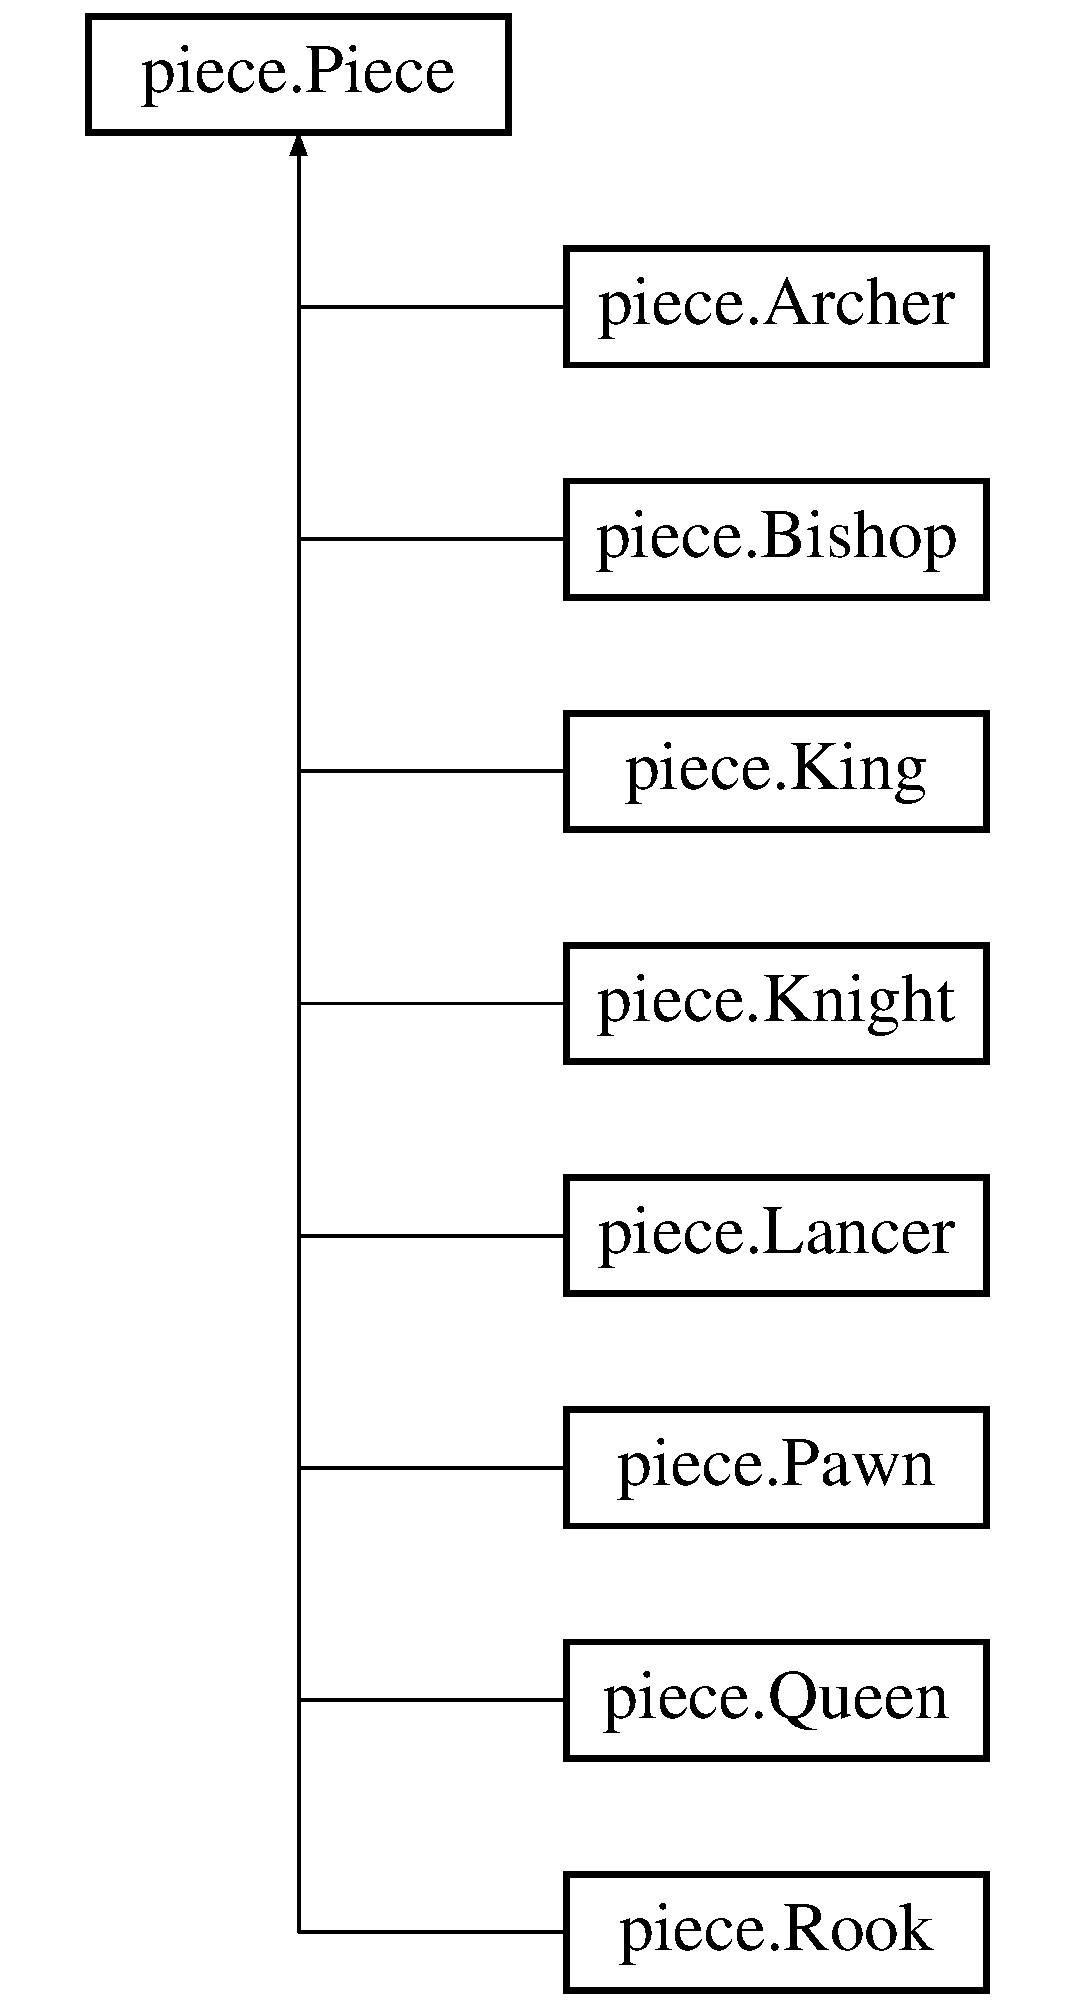
\includegraphics[height=9.000000cm]{classpiece_1_1_piece}
\end{center}
\end{figure}
\subsection*{Public Member Functions}
\begin{DoxyCompactItemize}
\item 
\hyperlink{classpiece_1_1_piece_a2a951c56b9c86a93fab817ddb7da4413}{Piece} (String piece\+\_\+name, \hyperlink{classchess_1_1_chess_board}{Chess\+Board} board, \hyperlink{enumchess_1_1_player}{Player} player)
\item 
boolean \hyperlink{classpiece_1_1_piece_a22f311f1704a5fff7041bf311a88bb80}{set\+Coordinate} (int x, int y)
\item 
void \hyperlink{classpiece_1_1_piece_a2b2074610fdf598443fcc3f0b1a32f13}{remove\+Self} ()
\item 
\hyperlink{classchess_1_1_chess_board}{Chess\+Board} \hyperlink{classpiece_1_1_piece_a1004705760b36db3185de90faaf76bbc}{get\+Chess\+Board} ()
\item 
void \hyperlink{classpiece_1_1_piece_a01948cad1916776f6a900c2918f395c3}{set\+Player} (\hyperlink{enumchess_1_1_player}{Player} player)
\item 
\hyperlink{enumchess_1_1_player}{Player} \hyperlink{classpiece_1_1_piece_ac2f9d5a3cef28997c6bfab69792a2898}{get\+Player} ()
\item 
int \hyperlink{classpiece_1_1_piece_a0b9fa85eb166a0290e7825daddd7d129}{get\+X\+\_\+coordinate} ()
\item 
int \hyperlink{classpiece_1_1_piece_a12a8ca4143a3d3937ad8071d9e29c171}{get\+Y\+\_\+coordinate} ()
\item 
String \hyperlink{classpiece_1_1_piece_afb5b4b2899fb574b421125c12e4adc31}{get\+Piece\+\_\+name} ()
\item 
void \hyperlink{classpiece_1_1_piece_a07277fb8549c95d3522223790bf8a7c5}{set\+Piece\+\_\+image\+\_\+path} (String piece\+\_\+image\+\_\+path)
\item 
String \hyperlink{classpiece_1_1_piece_a0e49c966ed4a5dde90300825502ae4fd}{get\+Piece\+\_\+image\+\_\+path} ()
\item 
boolean \hyperlink{classpiece_1_1_piece_a9e8b91312f7a03a15cc987b5f5a99989}{add\+To\+Coordinates\+If\+Valid} (Array\+List$<$ \hyperlink{classpiece_1_1_coordinate}{Coordinate} $>$ coords, int x, int y)
\item 
abstract Array\+List$<$ \hyperlink{classpiece_1_1_coordinate}{Coordinate} $>$ \hyperlink{classpiece_1_1_piece_a9ac176ed64bf25c3fdbf5668ba4011e4}{get\+Possible\+Move\+Coordinate} ()
\end{DoxyCompactItemize}
\subsection*{Protected Attributes}
\begin{DoxyCompactItemize}
\item 
\hypertarget{classpiece_1_1_piece_a670862c335c65ea88dce5269c9ce9bfb}{}String {\bfseries piece\+\_\+name}\label{classpiece_1_1_piece_a670862c335c65ea88dce5269c9ce9bfb}

\item 
\hypertarget{classpiece_1_1_piece_aedff76d42dc52074d88776c447d75aac}{}int {\bfseries x\+\_\+coordinate}\label{classpiece_1_1_piece_aedff76d42dc52074d88776c447d75aac}

\item 
\hypertarget{classpiece_1_1_piece_a5eb75915739d2aac27293242b4b062c3}{}int {\bfseries y\+\_\+coordinate}\label{classpiece_1_1_piece_a5eb75915739d2aac27293242b4b062c3}

\item 
\hypertarget{classpiece_1_1_piece_a7aef88c8a61c1cd4a469aa15393ae1c2}{}\hyperlink{enumchess_1_1_player}{Player} {\bfseries player}\label{classpiece_1_1_piece_a7aef88c8a61c1cd4a469aa15393ae1c2}

\item 
\hypertarget{classpiece_1_1_piece_a89bee87e940fc2718964d92e842517d7}{}\hyperlink{classchess_1_1_chess_board}{Chess\+Board} {\bfseries board}\label{classpiece_1_1_piece_a89bee87e940fc2718964d92e842517d7}

\item 
\hypertarget{classpiece_1_1_piece_af66e4d5f1b6324a93d43f7778be2da36}{}String {\bfseries piece\+\_\+image\+\_\+path}\label{classpiece_1_1_piece_af66e4d5f1b6324a93d43f7778be2da36}

\end{DoxyCompactItemize}


\subsection{Detailed Description}
Created by wangyiyi on 2/12/15.

\hyperlink{classpiece_1_1_piece}{Piece} Class 

\subsection{Constructor \& Destructor Documentation}
\hypertarget{classpiece_1_1_piece_a2a951c56b9c86a93fab817ddb7da4413}{}\index{piece\+::\+Piece@{piece\+::\+Piece}!Piece@{Piece}}
\index{Piece@{Piece}!piece\+::\+Piece@{piece\+::\+Piece}}
\subsubsection[{Piece}]{\setlength{\rightskip}{0pt plus 5cm}piece.\+Piece.\+Piece (
\begin{DoxyParamCaption}
\item[{String}]{piece\+\_\+name, }
\item[{{\bf Chess\+Board}}]{board, }
\item[{{\bf Player}}]{player}
\end{DoxyParamCaption}
)\hspace{0.3cm}{\ttfamily [inline]}}\label{classpiece_1_1_piece_a2a951c56b9c86a93fab817ddb7da4413}
Initialize a piece object 
\begin{DoxyParams}{Parameters}
{\em piece\+\_\+name} & set the piece name \\
\hline
{\em board} & the chess board where we put this piece \\
\hline
{\em player} & the player id \\
\hline
\end{DoxyParams}


\subsection{Member Function Documentation}
\hypertarget{classpiece_1_1_piece_a9e8b91312f7a03a15cc987b5f5a99989}{}\index{piece\+::\+Piece@{piece\+::\+Piece}!add\+To\+Coordinates\+If\+Valid@{add\+To\+Coordinates\+If\+Valid}}
\index{add\+To\+Coordinates\+If\+Valid@{add\+To\+Coordinates\+If\+Valid}!piece\+::\+Piece@{piece\+::\+Piece}}
\subsubsection[{add\+To\+Coordinates\+If\+Valid}]{\setlength{\rightskip}{0pt plus 5cm}boolean piece.\+Piece.\+add\+To\+Coordinates\+If\+Valid (
\begin{DoxyParamCaption}
\item[{Array\+List$<$ {\bf Coordinate} $>$}]{coords, }
\item[{int}]{x, }
\item[{int}]{y}
\end{DoxyParamCaption}
)\hspace{0.3cm}{\ttfamily [inline]}}\label{classpiece_1_1_piece_a9e8b91312f7a03a15cc987b5f5a99989}
Given coordinate (x, y), check whether the piece can move there.

If the piece can move to that coordinate, save (x, y) to coords.

If the piece cannot move anywhere further after reach that coordinate, like there is an another piece there, which blocks the way =$>$ return true; otherwise return false 
\begin{DoxyParams}{Parameters}
{\em coords} & the coordinates array list \\
\hline
{\em x} & the x coordinate to check \\
\hline
{\em y} & the y coordinate to check \\
\hline
\end{DoxyParams}
\begin{DoxyReturn}{Returns}
true if the piece at that coordinate is opponent\textquotesingle{}s piece or player\textquotesingle{}s piece, thus it will block the way. 
\end{DoxyReturn}
\hypertarget{classpiece_1_1_piece_a1004705760b36db3185de90faaf76bbc}{}\index{piece\+::\+Piece@{piece\+::\+Piece}!get\+Chess\+Board@{get\+Chess\+Board}}
\index{get\+Chess\+Board@{get\+Chess\+Board}!piece\+::\+Piece@{piece\+::\+Piece}}
\subsubsection[{get\+Chess\+Board}]{\setlength{\rightskip}{0pt plus 5cm}{\bf Chess\+Board} piece.\+Piece.\+get\+Chess\+Board (
\begin{DoxyParamCaption}
{}
\end{DoxyParamCaption}
)\hspace{0.3cm}{\ttfamily [inline]}}\label{classpiece_1_1_piece_a1004705760b36db3185de90faaf76bbc}
Chess\+Boarder getter \begin{DoxyReturn}{Returns}
board 
\end{DoxyReturn}
\hypertarget{classpiece_1_1_piece_a0e49c966ed4a5dde90300825502ae4fd}{}\index{piece\+::\+Piece@{piece\+::\+Piece}!get\+Piece\+\_\+image\+\_\+path@{get\+Piece\+\_\+image\+\_\+path}}
\index{get\+Piece\+\_\+image\+\_\+path@{get\+Piece\+\_\+image\+\_\+path}!piece\+::\+Piece@{piece\+::\+Piece}}
\subsubsection[{get\+Piece\+\_\+image\+\_\+path}]{\setlength{\rightskip}{0pt plus 5cm}String piece.\+Piece.\+get\+Piece\+\_\+image\+\_\+path (
\begin{DoxyParamCaption}
{}
\end{DoxyParamCaption}
)\hspace{0.3cm}{\ttfamily [inline]}}\label{classpiece_1_1_piece_a0e49c966ed4a5dde90300825502ae4fd}
Getter, return piece image path of this piece \begin{DoxyReturn}{Returns}
image path of this piece 
\end{DoxyReturn}
\hypertarget{classpiece_1_1_piece_afb5b4b2899fb574b421125c12e4adc31}{}\index{piece\+::\+Piece@{piece\+::\+Piece}!get\+Piece\+\_\+name@{get\+Piece\+\_\+name}}
\index{get\+Piece\+\_\+name@{get\+Piece\+\_\+name}!piece\+::\+Piece@{piece\+::\+Piece}}
\subsubsection[{get\+Piece\+\_\+name}]{\setlength{\rightskip}{0pt plus 5cm}String piece.\+Piece.\+get\+Piece\+\_\+name (
\begin{DoxyParamCaption}
{}
\end{DoxyParamCaption}
)\hspace{0.3cm}{\ttfamily [inline]}}\label{classpiece_1_1_piece_afb5b4b2899fb574b421125c12e4adc31}
Getter, return the piece name of this piece \begin{DoxyReturn}{Returns}
piece name of this piece 
\end{DoxyReturn}
\hypertarget{classpiece_1_1_piece_ac2f9d5a3cef28997c6bfab69792a2898}{}\index{piece\+::\+Piece@{piece\+::\+Piece}!get\+Player@{get\+Player}}
\index{get\+Player@{get\+Player}!piece\+::\+Piece@{piece\+::\+Piece}}
\subsubsection[{get\+Player}]{\setlength{\rightskip}{0pt plus 5cm}{\bf Player} piece.\+Piece.\+get\+Player (
\begin{DoxyParamCaption}
{}
\end{DoxyParamCaption}
)\hspace{0.3cm}{\ttfamily [inline]}}\label{classpiece_1_1_piece_ac2f9d5a3cef28997c6bfab69792a2898}
Getter, return player \begin{DoxyReturn}{Returns}
player 
\end{DoxyReturn}
\hypertarget{classpiece_1_1_piece_a9ac176ed64bf25c3fdbf5668ba4011e4}{}\index{piece\+::\+Piece@{piece\+::\+Piece}!get\+Possible\+Move\+Coordinate@{get\+Possible\+Move\+Coordinate}}
\index{get\+Possible\+Move\+Coordinate@{get\+Possible\+Move\+Coordinate}!piece\+::\+Piece@{piece\+::\+Piece}}
\subsubsection[{get\+Possible\+Move\+Coordinate}]{\setlength{\rightskip}{0pt plus 5cm}abstract Array\+List$<${\bf Coordinate}$>$ piece.\+Piece.\+get\+Possible\+Move\+Coordinate (
\begin{DoxyParamCaption}
{}
\end{DoxyParamCaption}
)\hspace{0.3cm}{\ttfamily [abstract]}}\label{classpiece_1_1_piece_a9ac176ed64bf25c3fdbf5668ba4011e4}
Get possible move coordinates for this piece

As this function is implemented in each subclass, it will return null.

\begin{DoxyReturn}{Returns}
Array\+List$<$\+Coordinate$>$ Object that contains all possible move coordinates. 
\end{DoxyReturn}
\hypertarget{classpiece_1_1_piece_a0b9fa85eb166a0290e7825daddd7d129}{}\index{piece\+::\+Piece@{piece\+::\+Piece}!get\+X\+\_\+coordinate@{get\+X\+\_\+coordinate}}
\index{get\+X\+\_\+coordinate@{get\+X\+\_\+coordinate}!piece\+::\+Piece@{piece\+::\+Piece}}
\subsubsection[{get\+X\+\_\+coordinate}]{\setlength{\rightskip}{0pt plus 5cm}int piece.\+Piece.\+get\+X\+\_\+coordinate (
\begin{DoxyParamCaption}
{}
\end{DoxyParamCaption}
)\hspace{0.3cm}{\ttfamily [inline]}}\label{classpiece_1_1_piece_a0b9fa85eb166a0290e7825daddd7d129}
Getter, return the x coordinate of this piece \begin{DoxyReturn}{Returns}
x coordinate of this piece 
\end{DoxyReturn}
\hypertarget{classpiece_1_1_piece_a12a8ca4143a3d3937ad8071d9e29c171}{}\index{piece\+::\+Piece@{piece\+::\+Piece}!get\+Y\+\_\+coordinate@{get\+Y\+\_\+coordinate}}
\index{get\+Y\+\_\+coordinate@{get\+Y\+\_\+coordinate}!piece\+::\+Piece@{piece\+::\+Piece}}
\subsubsection[{get\+Y\+\_\+coordinate}]{\setlength{\rightskip}{0pt plus 5cm}int piece.\+Piece.\+get\+Y\+\_\+coordinate (
\begin{DoxyParamCaption}
{}
\end{DoxyParamCaption}
)\hspace{0.3cm}{\ttfamily [inline]}}\label{classpiece_1_1_piece_a12a8ca4143a3d3937ad8071d9e29c171}
Getter, return the y coordinate of this piece \begin{DoxyReturn}{Returns}
y coordinate of this piece 
\end{DoxyReturn}
\hypertarget{classpiece_1_1_piece_a2b2074610fdf598443fcc3f0b1a32f13}{}\index{piece\+::\+Piece@{piece\+::\+Piece}!remove\+Self@{remove\+Self}}
\index{remove\+Self@{remove\+Self}!piece\+::\+Piece@{piece\+::\+Piece}}
\subsubsection[{remove\+Self}]{\setlength{\rightskip}{0pt plus 5cm}void piece.\+Piece.\+remove\+Self (
\begin{DoxyParamCaption}
{}
\end{DoxyParamCaption}
)\hspace{0.3cm}{\ttfamily [inline]}}\label{classpiece_1_1_piece_a2b2074610fdf598443fcc3f0b1a32f13}
\hyperlink{classpiece_1_1_piece}{Piece} removes itself from chess board \hypertarget{classpiece_1_1_piece_a22f311f1704a5fff7041bf311a88bb80}{}\index{piece\+::\+Piece@{piece\+::\+Piece}!set\+Coordinate@{set\+Coordinate}}
\index{set\+Coordinate@{set\+Coordinate}!piece\+::\+Piece@{piece\+::\+Piece}}
\subsubsection[{set\+Coordinate}]{\setlength{\rightskip}{0pt plus 5cm}boolean piece.\+Piece.\+set\+Coordinate (
\begin{DoxyParamCaption}
\item[{int}]{x, }
\item[{int}]{y}
\end{DoxyParamCaption}
)\hspace{0.3cm}{\ttfamily [inline]}}\label{classpiece_1_1_piece_a22f311f1704a5fff7041bf311a88bb80}
Set the coordinate of piece on chess board 
\begin{DoxyParams}{Parameters}
{\em x} & the x coordinate to put the piece \\
\hline
{\em y} & the y coordinate to put the piece \\
\hline
\end{DoxyParams}
\begin{DoxyReturn}{Returns}
if can put the piece at that coordinate, return true; otherwise return true. 
\end{DoxyReturn}
\hypertarget{classpiece_1_1_piece_a07277fb8549c95d3522223790bf8a7c5}{}\index{piece\+::\+Piece@{piece\+::\+Piece}!set\+Piece\+\_\+image\+\_\+path@{set\+Piece\+\_\+image\+\_\+path}}
\index{set\+Piece\+\_\+image\+\_\+path@{set\+Piece\+\_\+image\+\_\+path}!piece\+::\+Piece@{piece\+::\+Piece}}
\subsubsection[{set\+Piece\+\_\+image\+\_\+path}]{\setlength{\rightskip}{0pt plus 5cm}void piece.\+Piece.\+set\+Piece\+\_\+image\+\_\+path (
\begin{DoxyParamCaption}
\item[{String}]{piece\+\_\+image\+\_\+path}
\end{DoxyParamCaption}
)\hspace{0.3cm}{\ttfamily [inline]}}\label{classpiece_1_1_piece_a07277fb8549c95d3522223790bf8a7c5}
Setter, set the piece image path of this piece 
\begin{DoxyParams}{Parameters}
{\em piece\+\_\+image\+\_\+path} & \\
\hline
\end{DoxyParams}
\hypertarget{classpiece_1_1_piece_a01948cad1916776f6a900c2918f395c3}{}\index{piece\+::\+Piece@{piece\+::\+Piece}!set\+Player@{set\+Player}}
\index{set\+Player@{set\+Player}!piece\+::\+Piece@{piece\+::\+Piece}}
\subsubsection[{set\+Player}]{\setlength{\rightskip}{0pt plus 5cm}void piece.\+Piece.\+set\+Player (
\begin{DoxyParamCaption}
\item[{{\bf Player}}]{player}
\end{DoxyParamCaption}
)\hspace{0.3cm}{\ttfamily [inline]}}\label{classpiece_1_1_piece_a01948cad1916776f6a900c2918f395c3}
Setter, set player 
\begin{DoxyParams}{Parameters}
{\em player} & \\
\hline
\end{DoxyParams}


The documentation for this class was generated from the following file\+:\begin{DoxyCompactItemize}
\item 
piece/Piece.\+java\end{DoxyCompactItemize}

\hypertarget{classunit__test_1_1_piece_test}{}\section{unit\+\_\+test.\+Piece\+Test Class Reference}
\label{classunit__test_1_1_piece_test}\index{unit\+\_\+test.\+Piece\+Test@{unit\+\_\+test.\+Piece\+Test}}
\subsection*{Public Member Functions}
\begin{DoxyCompactItemize}
\item 
void \hyperlink{classunit__test_1_1_piece_test_a861ec95f06e77a56a6f0cd657c69c348}{test\+Get\+Player} ()  throws Exception 
\item 
void \hyperlink{classunit__test_1_1_piece_test_afebc3ef00ab575e3e289b55d73f70be6}{test\+Get\+Piece\+\_\+name} ()  throws Exception 
\item 
void \hyperlink{classunit__test_1_1_piece_test_aa161bcd95ec8e6989765bf31f03a52c8}{test\+Get\+Piece\+\_\+image\+\_\+path} ()  throws Exception 
\item 
void \hyperlink{classunit__test_1_1_piece_test_a146e52bc753bc9d53b1bdc7834392c69}{test\+Set\+Coordinate} ()  throws Exception
\item 
void \hyperlink{classunit__test_1_1_piece_test_a0f2f7f4c09b05623767b424f527ac2af}{test\+Remove\+Self} ()  throws Exception 
\end{DoxyCompactItemize}


\subsection{Member Function Documentation}
\hypertarget{classunit__test_1_1_piece_test_aa161bcd95ec8e6989765bf31f03a52c8}{}\index{unit\+\_\+test\+::\+Piece\+Test@{unit\+\_\+test\+::\+Piece\+Test}!test\+Get\+Piece\+\_\+image\+\_\+path@{test\+Get\+Piece\+\_\+image\+\_\+path}}
\index{test\+Get\+Piece\+\_\+image\+\_\+path@{test\+Get\+Piece\+\_\+image\+\_\+path}!unit\+\_\+test\+::\+Piece\+Test@{unit\+\_\+test\+::\+Piece\+Test}}
\subsubsection[{test\+Get\+Piece\+\_\+image\+\_\+path}]{\setlength{\rightskip}{0pt plus 5cm}void unit\+\_\+test.\+Piece\+Test.\+test\+Get\+Piece\+\_\+image\+\_\+path (
\begin{DoxyParamCaption}
{}
\end{DoxyParamCaption}
) throws Exception\hspace{0.3cm}{\ttfamily [inline]}}\label{classunit__test_1_1_piece_test_aa161bcd95ec8e6989765bf31f03a52c8}
Test whether the piece image path is correct \hypertarget{classunit__test_1_1_piece_test_afebc3ef00ab575e3e289b55d73f70be6}{}\index{unit\+\_\+test\+::\+Piece\+Test@{unit\+\_\+test\+::\+Piece\+Test}!test\+Get\+Piece\+\_\+name@{test\+Get\+Piece\+\_\+name}}
\index{test\+Get\+Piece\+\_\+name@{test\+Get\+Piece\+\_\+name}!unit\+\_\+test\+::\+Piece\+Test@{unit\+\_\+test\+::\+Piece\+Test}}
\subsubsection[{test\+Get\+Piece\+\_\+name}]{\setlength{\rightskip}{0pt plus 5cm}void unit\+\_\+test.\+Piece\+Test.\+test\+Get\+Piece\+\_\+name (
\begin{DoxyParamCaption}
{}
\end{DoxyParamCaption}
) throws Exception\hspace{0.3cm}{\ttfamily [inline]}}\label{classunit__test_1_1_piece_test_afebc3ef00ab575e3e289b55d73f70be6}
Test whether piece name is correct 
\begin{DoxyExceptions}{Exceptions}
{\em Exception} & \\
\hline
\end{DoxyExceptions}
\hypertarget{classunit__test_1_1_piece_test_a861ec95f06e77a56a6f0cd657c69c348}{}\index{unit\+\_\+test\+::\+Piece\+Test@{unit\+\_\+test\+::\+Piece\+Test}!test\+Get\+Player@{test\+Get\+Player}}
\index{test\+Get\+Player@{test\+Get\+Player}!unit\+\_\+test\+::\+Piece\+Test@{unit\+\_\+test\+::\+Piece\+Test}}
\subsubsection[{test\+Get\+Player}]{\setlength{\rightskip}{0pt plus 5cm}void unit\+\_\+test.\+Piece\+Test.\+test\+Get\+Player (
\begin{DoxyParamCaption}
{}
\end{DoxyParamCaption}
) throws Exception\hspace{0.3cm}{\ttfamily [inline]}}\label{classunit__test_1_1_piece_test_a861ec95f06e77a56a6f0cd657c69c348}
Test player id player id could only be 1 or 2; otherwise throw exception 
\begin{DoxyExceptions}{Exceptions}
{\em Exception} & \\
\hline
\end{DoxyExceptions}
\hypertarget{classunit__test_1_1_piece_test_a0f2f7f4c09b05623767b424f527ac2af}{}\index{unit\+\_\+test\+::\+Piece\+Test@{unit\+\_\+test\+::\+Piece\+Test}!test\+Remove\+Self@{test\+Remove\+Self}}
\index{test\+Remove\+Self@{test\+Remove\+Self}!unit\+\_\+test\+::\+Piece\+Test@{unit\+\_\+test\+::\+Piece\+Test}}
\subsubsection[{test\+Remove\+Self}]{\setlength{\rightskip}{0pt plus 5cm}void unit\+\_\+test.\+Piece\+Test.\+test\+Remove\+Self (
\begin{DoxyParamCaption}
{}
\end{DoxyParamCaption}
) throws Exception\hspace{0.3cm}{\ttfamily [inline]}}\label{classunit__test_1_1_piece_test_a0f2f7f4c09b05623767b424f527ac2af}
test whether a piece can remove itself correctly 
\begin{DoxyExceptions}{Exceptions}
{\em Exception} & \\
\hline
\end{DoxyExceptions}
\hypertarget{classunit__test_1_1_piece_test_a146e52bc753bc9d53b1bdc7834392c69}{}\index{unit\+\_\+test\+::\+Piece\+Test@{unit\+\_\+test\+::\+Piece\+Test}!test\+Set\+Coordinate@{test\+Set\+Coordinate}}
\index{test\+Set\+Coordinate@{test\+Set\+Coordinate}!unit\+\_\+test\+::\+Piece\+Test@{unit\+\_\+test\+::\+Piece\+Test}}
\subsubsection[{test\+Set\+Coordinate}]{\setlength{\rightskip}{0pt plus 5cm}void unit\+\_\+test.\+Piece\+Test.\+test\+Set\+Coordinate (
\begin{DoxyParamCaption}
{}
\end{DoxyParamCaption}
) throws Exception\hspace{0.3cm}{\ttfamily [inline]}}\label{classunit__test_1_1_piece_test_a146e52bc753bc9d53b1bdc7834392c69}
Test when call set\+Coordinate on a invalid coordinate, will false be returned ? 
\begin{DoxyExceptions}{Exceptions}
{\em Exception} & \\
\hline
\end{DoxyExceptions}


The documentation for this class was generated from the following file\+:\begin{DoxyCompactItemize}
\item 
src/unit\+\_\+test/Piece\+Test.\+java\end{DoxyCompactItemize}

\hypertarget{enumchessboard_1_1_player}{}\section{chessboard.\+Player Enum Reference}
\label{enumchessboard_1_1_player}\index{chessboard.\+Player@{chessboard.\+Player}}
\subsection*{Public Attributes}
\begin{DoxyCompactItemize}
\item 
\hypertarget{enumchessboard_1_1_player_a4e15274b111d24e3d62dc2a169072b97}{}{\bfseries W\+H\+I\+T\+E}\label{enumchessboard_1_1_player_a4e15274b111d24e3d62dc2a169072b97}

\item 
\hypertarget{enumchessboard_1_1_player_ab0345c4225cc8b29adb0fcc81996863f}{}{\bfseries B\+L\+A\+C\+K}\label{enumchessboard_1_1_player_ab0345c4225cc8b29adb0fcc81996863f}

\end{DoxyCompactItemize}


\subsection{Detailed Description}
Created by wangyiyi on 2/17/15. Our chess game will support 2 types of players\+: W\+H\+I\+T\+E and B\+L\+A\+C\+K 

The documentation for this enum was generated from the following file\+:\begin{DoxyCompactItemize}
\item 
src/chessboard/Player.\+java\end{DoxyCompactItemize}

\hypertarget{classpiece_1_1_queen}{}\section{piece.\+Queen Class Reference}
\label{classpiece_1_1_queen}\index{piece.\+Queen@{piece.\+Queen}}
Inheritance diagram for piece.\+Queen\+:\begin{figure}[H]
\begin{center}
\leavevmode
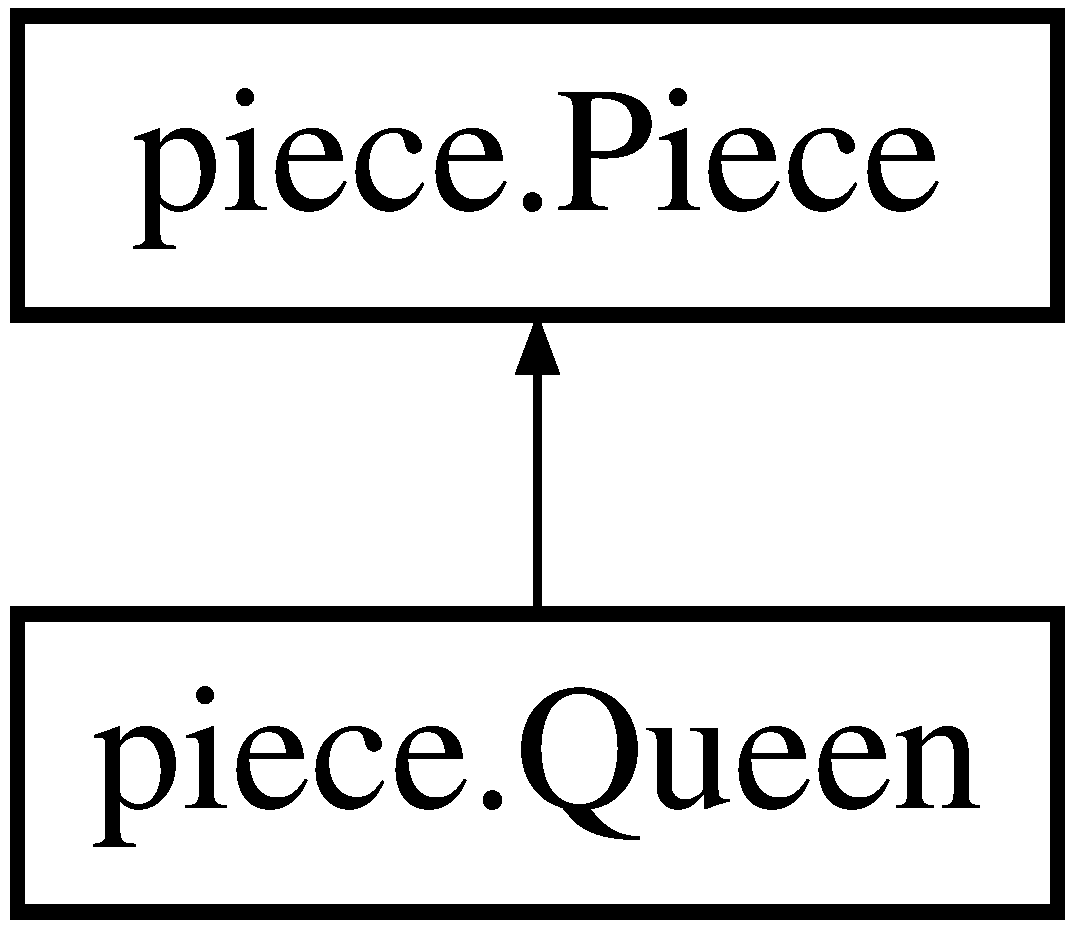
\includegraphics[height=2.000000cm]{classpiece_1_1_queen}
\end{center}
\end{figure}
\subsection*{Public Member Functions}
\begin{DoxyCompactItemize}
\item 
\hyperlink{classpiece_1_1_queen_ab07236b4d2d74af4752527d4be4d0e37}{Queen} (\hyperlink{classchess_1_1_chess_board}{Chess\+Board} board, \hyperlink{enumchess_1_1_player}{Player} player)
\item 
Array\+List$<$ \hyperlink{classpiece_1_1_coordinate}{Coordinate} $>$ \hyperlink{classpiece_1_1_queen_acaedb2b5fe8ca1ffac745ef059d2466c}{get\+Possible\+Move\+Coordinate} ()
\end{DoxyCompactItemize}
\subsection*{Additional Inherited Members}


\subsection{Detailed Description}
Created by wangyiyi on 2/12/15. 

\subsection{Constructor \& Destructor Documentation}
\hypertarget{classpiece_1_1_queen_ab07236b4d2d74af4752527d4be4d0e37}{}\index{piece\+::\+Queen@{piece\+::\+Queen}!Queen@{Queen}}
\index{Queen@{Queen}!piece\+::\+Queen@{piece\+::\+Queen}}
\subsubsection[{Queen}]{\setlength{\rightskip}{0pt plus 5cm}piece.\+Queen.\+Queen (
\begin{DoxyParamCaption}
\item[{{\bf Chess\+Board}}]{board, }
\item[{{\bf Player}}]{player}
\end{DoxyParamCaption}
)\hspace{0.3cm}{\ttfamily [inline]}}\label{classpiece_1_1_queen_ab07236b4d2d74af4752527d4be4d0e37}
Constructor\+: initialize \hyperlink{classpiece_1_1_queen}{Queen} Object 
\begin{DoxyParams}{Parameters}
{\em board} & the board that we are currently using \\
\hline
{\em player} & the player that holds the piece \\
\hline
\end{DoxyParams}


\subsection{Member Function Documentation}
\hypertarget{classpiece_1_1_queen_acaedb2b5fe8ca1ffac745ef059d2466c}{}\index{piece\+::\+Queen@{piece\+::\+Queen}!get\+Possible\+Move\+Coordinate@{get\+Possible\+Move\+Coordinate}}
\index{get\+Possible\+Move\+Coordinate@{get\+Possible\+Move\+Coordinate}!piece\+::\+Queen@{piece\+::\+Queen}}
\subsubsection[{get\+Possible\+Move\+Coordinate}]{\setlength{\rightskip}{0pt plus 5cm}Array\+List$<${\bf Coordinate}$>$ piece.\+Queen.\+get\+Possible\+Move\+Coordinate (
\begin{DoxyParamCaption}
{}
\end{DoxyParamCaption}
)\hspace{0.3cm}{\ttfamily [inline]}}\label{classpiece_1_1_queen_acaedb2b5fe8ca1ffac745ef059d2466c}
Get all possible move coordinates for this queen piece at current coordinate \begin{DoxyVerb}   @   @   @
    @  @  @         P: this piece
     @ @ @          @: Possible coordinates to move
   @ @ P @ @
     @ @ @
    @  @  @
   @   @   @
\end{DoxyVerb}


\begin{DoxyReturn}{Returns}
Array\+List$<$\+Coordinate$>$ Object that contains all possible move coordinates. 
\end{DoxyReturn}


The documentation for this class was generated from the following file\+:\begin{DoxyCompactItemize}
\item 
piece/Queen.\+java\end{DoxyCompactItemize}

\hypertarget{classunit__test_1_1_queen_test}{}\section{unit\+\_\+test.\+Queen\+Test Class Reference}
\label{classunit__test_1_1_queen_test}\index{unit\+\_\+test.\+Queen\+Test@{unit\+\_\+test.\+Queen\+Test}}
\subsection*{Public Member Functions}
\begin{DoxyCompactItemize}
\item 
void \hyperlink{classunit__test_1_1_queen_test_ab5a3a82a47fb0d8ebf715f8718d4c79f}{test\+Get\+Possible\+Move\+Coordinate} ()  throws Exception 
\end{DoxyCompactItemize}


\subsection{Member Function Documentation}
\hypertarget{classunit__test_1_1_queen_test_ab5a3a82a47fb0d8ebf715f8718d4c79f}{}\index{unit\+\_\+test\+::\+Queen\+Test@{unit\+\_\+test\+::\+Queen\+Test}!test\+Get\+Possible\+Move\+Coordinate@{test\+Get\+Possible\+Move\+Coordinate}}
\index{test\+Get\+Possible\+Move\+Coordinate@{test\+Get\+Possible\+Move\+Coordinate}!unit\+\_\+test\+::\+Queen\+Test@{unit\+\_\+test\+::\+Queen\+Test}}
\subsubsection[{test\+Get\+Possible\+Move\+Coordinate}]{\setlength{\rightskip}{0pt plus 5cm}void unit\+\_\+test.\+Queen\+Test.\+test\+Get\+Possible\+Move\+Coordinate (
\begin{DoxyParamCaption}
{}
\end{DoxyParamCaption}
) throws Exception\hspace{0.3cm}{\ttfamily [inline]}}\label{classunit__test_1_1_queen_test_ab5a3a82a47fb0d8ebf715f8718d4c79f}
test valid possible moves 
\begin{DoxyExceptions}{Exceptions}
{\em Exception} & \\
\hline
\end{DoxyExceptions}


The documentation for this class was generated from the following file\+:\begin{DoxyCompactItemize}
\item 
unit\+\_\+test/Queen\+Test.\+java\end{DoxyCompactItemize}

\hypertarget{classpiece_1_1_rook}{}\section{piece.\+Rook Class Reference}
\label{classpiece_1_1_rook}\index{piece.\+Rook@{piece.\+Rook}}
Inheritance diagram for piece.\+Rook\+:\begin{figure}[H]
\begin{center}
\leavevmode
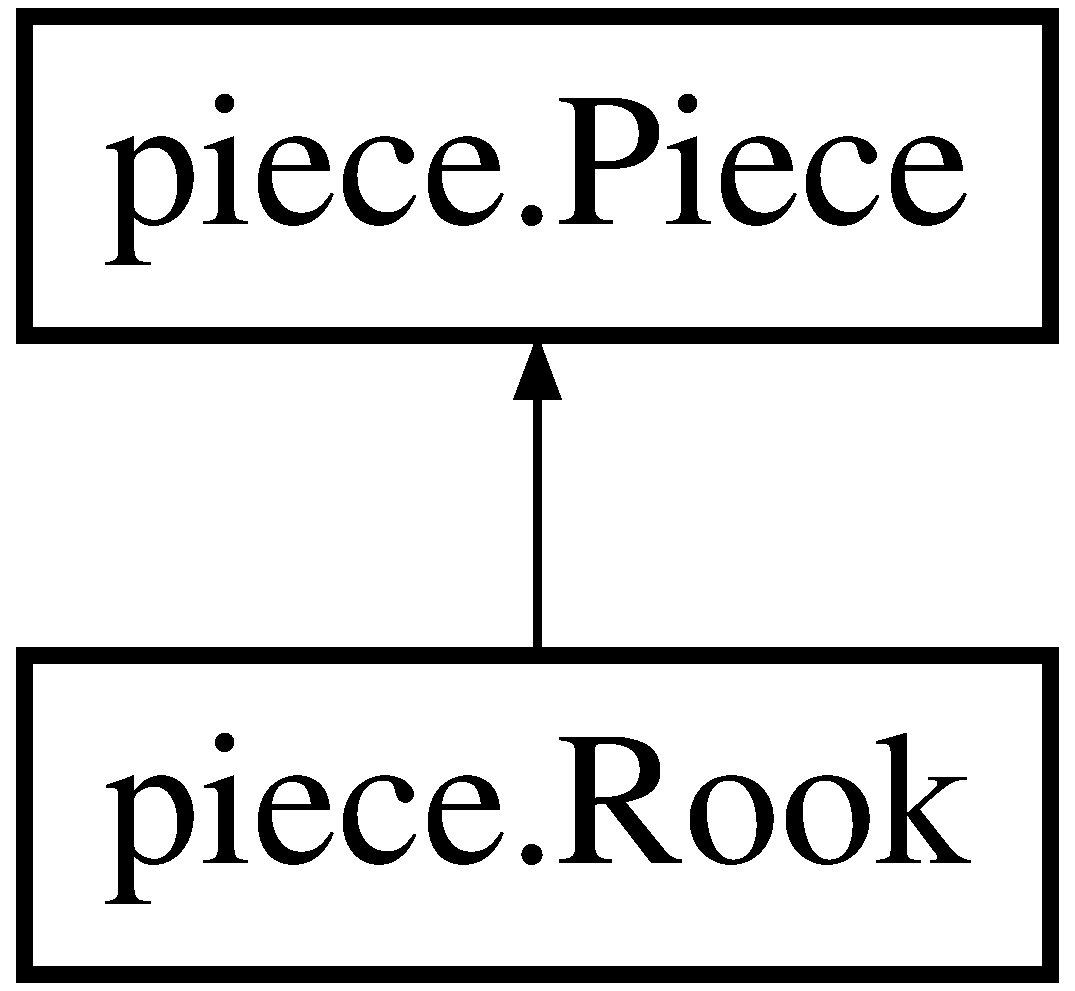
\includegraphics[height=2.000000cm]{classpiece_1_1_rook}
\end{center}
\end{figure}
\subsection*{Public Member Functions}
\begin{DoxyCompactItemize}
\item 
\hyperlink{classpiece_1_1_rook_a0a79f7132a0afa353f13cb3a526e8bc7}{Rook} (\hyperlink{classchess_1_1_chess_board}{Chess\+Board} board, \hyperlink{enumchess_1_1_player}{Player} player)
\item 
Array\+List$<$ \hyperlink{classpiece_1_1_coordinate}{Coordinate} $>$ \hyperlink{classpiece_1_1_rook_ae4bd548b81c1224b1db56517315063aa}{get\+Possible\+Move\+Coordinate} ()
\end{DoxyCompactItemize}
\subsection*{Additional Inherited Members}


\subsection{Detailed Description}
Created by wangyiyi on 2/12/15. 

\subsection{Constructor \& Destructor Documentation}
\hypertarget{classpiece_1_1_rook_a0a79f7132a0afa353f13cb3a526e8bc7}{}\index{piece\+::\+Rook@{piece\+::\+Rook}!Rook@{Rook}}
\index{Rook@{Rook}!piece\+::\+Rook@{piece\+::\+Rook}}
\subsubsection[{Rook}]{\setlength{\rightskip}{0pt plus 5cm}piece.\+Rook.\+Rook (
\begin{DoxyParamCaption}
\item[{{\bf Chess\+Board}}]{board, }
\item[{{\bf Player}}]{player}
\end{DoxyParamCaption}
)\hspace{0.3cm}{\ttfamily [inline]}}\label{classpiece_1_1_rook_a0a79f7132a0afa353f13cb3a526e8bc7}
Constructor\+: initialize a \hyperlink{classpiece_1_1_rook}{Rook} Object 
\begin{DoxyParams}{Parameters}
{\em board} & \\
\hline
{\em player} & \\
\hline
\end{DoxyParams}


\subsection{Member Function Documentation}
\hypertarget{classpiece_1_1_rook_ae4bd548b81c1224b1db56517315063aa}{}\index{piece\+::\+Rook@{piece\+::\+Rook}!get\+Possible\+Move\+Coordinate@{get\+Possible\+Move\+Coordinate}}
\index{get\+Possible\+Move\+Coordinate@{get\+Possible\+Move\+Coordinate}!piece\+::\+Rook@{piece\+::\+Rook}}
\subsubsection[{get\+Possible\+Move\+Coordinate}]{\setlength{\rightskip}{0pt plus 5cm}Array\+List$<${\bf Coordinate}$>$ piece.\+Rook.\+get\+Possible\+Move\+Coordinate (
\begin{DoxyParamCaption}
{}
\end{DoxyParamCaption}
)\hspace{0.3cm}{\ttfamily [inline]}}\label{classpiece_1_1_rook_ae4bd548b81c1224b1db56517315063aa}
Get all possible move coordinates for this rook piece at current coordinate \begin{DoxyVerb}    @
    @          P: this piece
    @          @: Possible coordinates to move
\end{DoxyVerb}
 @ @ @ P @ @ @ @ @ @

\begin{DoxyReturn}{Returns}
Array\+List$<$\+Coordinate$>$ Object 
\end{DoxyReturn}


The documentation for this class was generated from the following file\+:\begin{DoxyCompactItemize}
\item 
piece/Rook.\+java\end{DoxyCompactItemize}

\hypertarget{classunit__test_1_1_rook_test}{}\section{unit\+\_\+test.\+Rook\+Test Class Reference}
\label{classunit__test_1_1_rook_test}\index{unit\+\_\+test.\+Rook\+Test@{unit\+\_\+test.\+Rook\+Test}}
\subsection*{Public Member Functions}
\begin{DoxyCompactItemize}
\item 
void \hyperlink{classunit__test_1_1_rook_test_a91c1e890a97ea5fa867acef1a4a0266d}{test\+Get\+Possible\+Move\+Coordinate} ()  throws Exception 
\end{DoxyCompactItemize}


\subsection{Member Function Documentation}
\hypertarget{classunit__test_1_1_rook_test_a91c1e890a97ea5fa867acef1a4a0266d}{}\index{unit\+\_\+test\+::\+Rook\+Test@{unit\+\_\+test\+::\+Rook\+Test}!test\+Get\+Possible\+Move\+Coordinate@{test\+Get\+Possible\+Move\+Coordinate}}
\index{test\+Get\+Possible\+Move\+Coordinate@{test\+Get\+Possible\+Move\+Coordinate}!unit\+\_\+test\+::\+Rook\+Test@{unit\+\_\+test\+::\+Rook\+Test}}
\subsubsection[{test\+Get\+Possible\+Move\+Coordinate}]{\setlength{\rightskip}{0pt plus 5cm}void unit\+\_\+test.\+Rook\+Test.\+test\+Get\+Possible\+Move\+Coordinate (
\begin{DoxyParamCaption}
{}
\end{DoxyParamCaption}
) throws Exception\hspace{0.3cm}{\ttfamily [inline]}}\label{classunit__test_1_1_rook_test_a91c1e890a97ea5fa867acef1a4a0266d}
test valid possible moves 
\begin{DoxyExceptions}{Exceptions}
{\em Exception} & \\
\hline
\end{DoxyExceptions}


The documentation for this class was generated from the following file\+:\begin{DoxyCompactItemize}
\item 
src/unit\+\_\+test/Rook\+Test.\+java\end{DoxyCompactItemize}

%--- End generated contents ---

% Index
\backmatter
\newpage
\phantomsection
\clearemptydoublepage
\addcontentsline{toc}{chapter}{Index}
\printindex

\end{document}
